\documentclass[preprint,12pt]{elsarticle}

\usepackage{amsmath,amssymb}
\usepackage{graphicx}
\usepackage{booktabs}
\usepackage{array}
\usepackage{pdflscape}
\usepackage{enumitem}
\usepackage{hyperref}

\journal{Journal of Route Optimization Studies}

\begin{document}

\begin{frontmatter}

\title{Economic Outlier Detection in Routing Networks:\\
A Marginal Analysis Framework for Fixed and Optimized Routes}

\author{Abrahim Borgi}
\affiliation{organization={Senior Business Intelligence Analyst, North Media A/S},
            city={Copenhagen},
            country={Denmark}}

\begin{abstract}
This article investigates economic outlier detection in routing networks through a marginal contribution framework. A route unit is treated as economically outlying when removing it, alone or as part of a subset, improves route contribution margin after accounting for lost revenue and saved route cost. The article distinguishes between two reference structures: Type~1 evaluates removal under the observed route sequence, while Type~2 re-optimizes the retained route before evaluating the same economic question. Exact subset evaluation is used as a benchmark, and a hybrid search strategy is validated for larger route instances where exhaustive evaluation is infeasible. Applied to operational route data, the framework identifies economic outliers in a large share of route profiles, but typically removes only a small share of addresses. Modeled cost savings exceed revenue losses in all main route segments, producing positive contribution-margin effects. Type~1 generally yields larger marginal improvements, whereas Type~2 provides a stricter diagnosis that separates route-unit economics from inherited sequence inefficiency. Sensitivity analysis shows that route-level incidence is more stable than the exact selected address subset, especially across alternative cost and revenue profiles.
\end{abstract}

\begin{keyword}
route optimization \sep outlier detection \sep marginal analysis \sep contribution margin \sep vehicle routing
\end{keyword}

\end{frontmatter}

\section{Introduction}
\label{sec:introduction}

Existing operational routes can contain stops, or more generally route units, that are economically inefficient. In practice, such units are often recognized through geography: they may appear isolated, peripheral, or expensive to serve. However, geographical inconvenience alone is not sufficient to determine whether a route unit should be removed. The relevant decision criterion is economic. A route unit should be evaluated by the trade-off between the value it contributes and the routing and service cost it induces within the surrounding route structure.

This article studies that trade-off through a marginal perspective. Rather than asking whether a stop looks inefficient in isolation, the analysis asks what happens to route contribution margin when one route unit, or a subset of route units, is removed from an existing route. The object of interest is therefore not a statistical anomaly, but an economically defined outlier: a route unit or subset whose removal improves the contribution margin of the route under a clearly specified reference structure.

Two reference structures are central. In the first, the current route sequence is treated as fixed, which reflects operational settings in which the established service order is preserved. In the second, the remaining route is re-optimized after removal. This distinction is important because a historically inherited route order may itself be inefficient. Re-optimization removes this sequencing bias and evaluates the economic effect of removal relative to a best-available ordering of the retained route units.

The route is represented only to the extent needed for the economic analysis. Route units are modeled as vertices, directed travel costs as arcs, and the routing instance as an asymmetric distance or cost matrix. This representation supports both fixed-sequence evaluation and repeated route re-optimization without turning the paper into a general graph-theoretic treatment.

The central research idea is therefore the following: can economically harmful route units or subsets be identified by their marginal effect on route contribution margin under fixed and optimized route structures? To address this question, the paper makes four methodological contributions:
\begin{enumerate}[label=(\roman*)]
\item it formalizes an economic outlier concept based on marginal contribution margin rather than distance alone;
\item it distinguishes explicitly between fixed-sequence and optimized-sequence reference routes;
\item it uses exhaustive subset evaluation as a theoretical benchmark for exact outlier detection; and
\item it develops a hybrid search strategy that combines subset screening with repeated route solving to make the framework computationally practical.
\end{enumerate}

These contributions motivate the following research questions:
\begin{enumerate}[label=RQ\arabic*.,leftmargin=*]
\item How does economic outlier identification differ between fixed and optimized route sequences?
\item To what extent do subset effects reveal economically harmful groups that are not detected by single-stop analysis?
\item How closely can a hybrid search approximate exhaustive subset evaluation while reducing computational effort?
\item How sensitive are outlier classifications to assumptions about route-unit value and route cost?
\end{enumerate}

Figure~\ref{fig:empirical-spatial-context} provides a spatial overview of the empirical route network, while Figure~\ref{fig:route-examples} illustrates how route units, route sequence, and local geography enter the analysis at the individual-route level. The examples show both compact urban routing and more dispersed routing structures, emphasizing why economic outlier detection must account for the marginal interaction between address value, local service work, and inter-unit travel rather than distance alone.

\begin{figure}[t]
\centering

\includegraphics[width=0.72\textwidth]{\detokenize{_img/map_overview.png}}
\caption{Spatial overview of the empirical route network.}
\label{fig:empirical-spatial-context}
\end{figure}

\begin{figure}[t]
\centering

\includegraphics[width=0.49\textwidth]{\detokenize{_img/route.png}}

\includegraphics[width=0.49\textwidth]{\detokenize{_img/route2.png}}
\caption{Examples of individual route structures with ordered route units and connecting route segments.}
\label{fig:route-examples}
\end{figure}

The remainder of the paper is organized as follows. Section~\ref{sec:problem-statement-related-work} defines the problem formally and positions the study relative to existing literature. Section~\ref{sec:theoretical-framework} presents the theoretical framework for fixed and optimized routes. Section~\ref{sec:methodology} describes the exact and hybrid solution strategies, and Section~\ref{sec:implementation} summarizes the implementation, data, and computational setup. Section~\ref{sec:analysis-results} presents the empirical analysis, after which Sections~\ref{sec:discussion} and \ref{sec:conclusion} discuss implications and conclude the paper.

\section{Problem Statement and Related Work}
\label{sec:problem-statement-related-work}

This section formalizes economic outlier detection in routing networks as a graph problem and positions the framework relative to related work.

\subsection{Problem Statement}
\label{subsec:problem-statement}

The analysis considers an existing route composed of route units, where a route unit may represent either a single stop or an operationally aggregated group of stops. Define the route instance as
\[
\mathrm{GR}:=(R,D,p,o,L_u),
\]
where $R$ denotes the route units under analysis, $D = [d_{ij}]$ is an asymmetric distance matrix, $p=(p_i)_{i \in R}$ records the number of mailboxes associated with each route unit, $o=(o_i)_{i\in R}$ records the economic value or revenue associated with each route unit, and $L_u$ denotes the internal length or work component of route unit $u$. For a candidate removal subset $S \subseteq R$, the retained route is $R \setminus S$.

The economic objective is the route contribution margin. Let $N(A)=\sum_{u_i\in A}p_i$ denote the number of mailboxes in a set of route units $A\subseteq R$, and let
\[
O(A)=\sum_{u_i\in A}o_i
\]
denote the total economic value retained when serving $A$. This formulation does not require a constant revenue per mailbox; route units may have heterogeneous values. Let $\mathrm{APR}$ denote the cost rate applied to the route-length or work measure.

Route length is not only the distance between route units. For an ordered route $\pi=(u_{\pi(1)},\ldots,u_{\pi(k)})$, the fixed-sequence route length is defined as
\[
L(\pi)=
\sum_{t=1}^{k}L_{u_{\pi(t)}}
+\sum_{t=1}^{k-1}d_{\pi(t),\pi(t+1)} ,
\]
with an additional return term when the route is closed. The internal component $L_u$ captures within-unit traversal and operational work at the stop, such as service time, walking distance, or address-level handling effort, converted into the same cost-driving unit as the travel matrix. Under a fixed route sequence, contribution margin is therefore
\[
DG(R)=O(R)-\mathrm{APR}\cdot L(R).
\]
Under an optimized route sequence, the corresponding quantity is
\[
DG^*(R)=O(R)-\mathrm{APR}\cdot L^*(R),
\]
where $L^*(R)$ is the optimized route length obtained after re-ordering the retained route units while preserving the internal components $L_u$.

The marginal effect of removing a subset $S$ is then defined as
\[
C_2(S) = DG(R \setminus S) - DG(R)
\]
for the fixed-sequence case, and as
\[
C_2^*(S) = DG^*(R \setminus S) - DG^*(R)
\]
for the optimized-sequence case. The interpretation is direct: if $C_2(S) > 0$ or $C_2^*(S) > 0$, removing $S$ improves contribution margin relative to the relevant reference route.

This marginal improvement criterion alone is not sufficient for the outlier concept used in the paper. Let $z > 0$ denote a threshold for economically meaningful improvement. A subset $S \subseteq R$ is treated as an outlier subset only if its removal exceeds the threshold and the improvement is not preserved under arbitrary enlargement. Depending on the reference structure, this means either
\[
\begin{cases}
C_2(S) > z,\\
\exists\, S' \supset S \text{ such that } C_2(S') < z,
\end{cases}
\]
or
\[
\begin{cases}
C_2^*(S) > z,\\
\exists\, S' \supset S \text{ such that } C_2^*(S') < z.
\end{cases}
\]
The superset condition matters because the objective is not merely to find subsets with positive removal effects, but to identify economically harmful subsets whose effect is locally significant relative to larger removals.

This formulation gives rise to two distinct problem variants:
\begin{enumerate}[label=(\arabic*)]
\item \textbf{Type 1: Fixed sequence.} The subset $S$ is removed, and the remaining route $R \setminus S$ is evaluated under the preserved relative order inherited from the original route.
\item \textbf{Type 2: Optimized sequence.} The subset $S$ is removed, and the remaining route is solved again under an optimized ordering before its contribution margin is evaluated.
\end{enumerate}

Subsets are essential to the problem definition. Some route units may be only mildly unprofitable on their own but economically harmful in combination with nearby or structurally linked units. The task is therefore not equivalent to ranking individual stops by local inconvenience or marginal cost. It is a subset-evaluation problem in which interaction effects can be decisive.

The computational challenge follows immediately from the subset structure. The number of candidate removal subsets grows as $2^{|R|}$, and Type~2 additionally requires a route optimization for each evaluated subset. Exact evaluation is therefore theoretically transparent but computationally expensive, which motivates the hybrid search methods developed later in the paper.

\subsection{Related Work}
\label{subsec:related-work}

The broader optimization context is the literature on routing problems with profits. In the synthesis of Feillet et al.~\cite{feillet2005tsp_profits}, customers are associated with value or profit, and routing decisions trade collected value against travel cost or route feasibility. This perspective covers well-known families such as the Profitable Tour Problem, the Orienteering Problem, and the Prize-Collecting Traveling Salesman Problem \cite{balas1989prize,feillet2005tsp_profits,chao1996team_orienteering}. The common question in that literature is approximately which customers should be included when constructing a profitable route. The present work instead starts from an existing route and asks which route units, or subsets of route units, have a harmful marginal economic contribution to that route.

The closest related work is therefore customer-selection research that evaluates service decisions through marginal profitability. In particular, Aksen and Aras~\cite{aksen2006customer_selection} study customer selection and profit maximization in a vehicle routing setting and propose an iterative marginal profit analysis (iMPA), recognizing that the attractiveness of serving a customer depends on the routing cost created by that customer. This is conceptually close to the present framework, and the paper does not claim novelty for combining customer value and routing cost or for evaluating removal through a marginal economic lens. The distinction considered here lies elsewhere.

The present framework is formulated primarily as a diagnostic analysis of an existing route rather than as a constructive customer-selection model. Its object of interest is a candidate subset $S \subseteq R$, which makes subset-level interactions explicit: a group of route units may be economically harmful even when none of its members appears sufficiently harmful in isolation. In addition, the framework distinguishes between two route-reference structures: Type~1 evaluates $C_2(S)=DG(R\setminus S)-DG(R)$ under the current operating sequence, whereas Type~2 evaluates $C_2^*(S)=DG^*(R\setminus S)-DG^*(R)$ after re-optimizing the remaining route. This yields two complementary diagnostic interpretations, depending on whether the analyst wishes to preserve or abstract from inefficiency in the current route order. The economic-outlier interpretation is then made explicit through the threshold $z$ and the subset/superset criterion introduced later in the paper. Removal and reinsertion are also widely used as search operators in large neighborhood search \cite{pisinger2010large}, but there removal primarily serves the optimization process itself, whereas here removal is the object of economic analysis.

\section{Theoretical Framework}
\label{sec:theoretical-framework}

This section formalizes the economic outlier framework for a single route. The purpose is to separate three elements that are often conflated in operational route analysis: the representation of the route, the economic contribution of the route units, and the reference structure against which removal is evaluated. The framework covers two cases only: Type~1, where the route order is fixed, and Type~2, where the remaining route is re-optimized after removal.

\subsection{Route Representation}
\label{subsec:route-representation}

Let a route be represented by a finite set of route units
\[
R=\{u_1,\ldots,u_n\}.
\]
A route unit may correspond to a single address or to a structured group of addresses treated as one operational unit. Each unit $u_i$ has a mailbox count $p_i$, an economic value $o_i$, and an internal route component $L_{u_i}$. 
The retained economic value of a subset $A\subseteq R$ is
\[
O(A)=\sum_{u_i\in A}o_i.
\]

Travel between route units is represented by an asymmetric distance matrix
\[
D=[d_{ij}], \qquad d_{ij}\geq 0,
\]
where $d_{ij}$ is the travel cost or distance from route unit $u_i$ to route unit $u_j$. Asymmetry is allowed because travel times and distances may depend on direction, road access, one-way streets, or entry and exit points of structured route units.

The framework includes both a Hamiltonian cycle case, referred to as the TSP case, and a Hamiltonian path case, referred to as the HPP case. 
The definitions are closely related, differing only in the calculation of $L(\pi)$ or $L^*(\pi)$.

For a fixed sequence
\[
\pi=(u_{\pi(1)},\ldots,u_{\pi(k)})
\]
the route length is
\[
\text{HPP CASE: }L(\pi)=\sum_{t=1}^{k}L_{u_{\pi(t)}}+
\sum_{t=1}^{k-1}d_{\pi(t),\pi(t+1)}.
\]
\[
\text{TSP CASE: }L(\pi)=\sum_{t=1}^{k}L_{u_{\pi(t)}}+
\sum_{t=1}^{k}d_{\pi(t),\pi((t \text{ mod } k)+1)}.
\]
The internal term $L_u$ captures within-unit traversal and stop-level work, such as service time, walking inside a route unit, or address-level handling effort, expressed in the same cost-driving unit as the inter-unit travel measure. If the route is closed, a return term $d_{\pi(k),\pi(1)}$ is added. If the route is open, the route is interpreted as a Hamiltonian path and no return term is included.

For a set of route units $A\subseteq R$, the optimized length is defined as
\[
L^*(A)=
\min_{\pi\in\mathcal{P}(A)}
\left(
\sum_{u_i\in A}L_{u_i}
+\sum_{t=1}^{|A|-1}d_{\pi(t),\pi(t+1)}
\right),
\]
with the same closed-route adjustment when the problem is specified as TSP rather than HPP. Thus, $L(A)$ denotes the length induced by an existing sequence, whereas $L^*(A)$ denotes the best length under an optimized sequence.

\subsection{Contribution Margin}
\label{subsec:contribution-margin}

The economic objective is route contribution margin. Let $\mathrm{APR}$ denote the unit cost rate applied to the generalized route-length measure. Under a fixed sequence, the contribution margin of route $R$ is
\[
DG(R)=O(R)-\mathrm{APR}\cdot L(R).
\]
For a candidate removal subset $S\subseteq R$, the marginal effect of removal is
\[
C_2(S)=DG(R\setminus S)-DG(R).
\]
Expanding the expression gives
\[
C_2(S)
=O(R\setminus S)-O(R)
-\mathrm{APR}\cdot\bigl(L(R\setminus S)-L(R)\bigr).
\]
The first term is the value lost by removing the route units in $S$. The second term is the routing and service-work cost saved, expressed through the change in generalized route length. Removal is economically attractive only when the saved cost exceeds the lost value.

For the optimized reference structure, the analogous contribution margin is
\[
DG^*(R)=O(R)-\mathrm{APR}\cdot L^*(R),
\]
and the marginal removal effect is
\[
C_2^*(S)=DG^*(R\setminus S)-DG^*(R).
\]
Equivalently,
\[
C_2^*(S)
=O(R\setminus S)-O(R)
-\mathrm{APR}\cdot\bigl(L^*(R\setminus S)-L^*(R)\bigr).
\]
Both $C_2(S)$ and $C_2^*(S)$ are measured in the same economic unit as the contribution margin. A positive value means that removing $S$ improves the route economically under the relevant reference structure.

\subsection{Economic Outlier Definition}
\label{subsec:economic-outlier-definition}

The framework defines outliers economically rather than statistically. A route unit is not an outlier because it is geographically distant or visually isolated; it is an outlier if its removal produces a meaningful improvement in contribution margin relative to the specified route reference.

Let $z>0$ be a threshold for economically meaningful improvement. For a fixed-sequence reference, a subset $S\subseteq R$ is an economic outlier subset if
\[
\begin{cases}
C_2(S)>z,\\
\exists\, S'\supset S \text{ such that } C_2(S')<z.
\end{cases}
\]
For an optimized-sequence reference, the corresponding definition is
\[
\begin{cases}
C_2^*(S)>z,\\
\exists\, S'\supset S \text{ such that } C_2^*(S')<z.
\end{cases}
\]
The threshold condition ensures that the improvement is not merely numerical noise. The superset condition gives the definition a local economic interpretation: $S$ is harmful enough to remove, but indiscriminate enlargement of the removed set does not necessarily remain profitable. This prevents the analysis from collapsing into a trivial preference for serving fewer and fewer route units.

The subset formulation is central. A single route unit may not satisfy the outlier condition by itself, while a pair or group may do so because the group jointly creates a costly detour. Conversely, a unit that appears harmful alone may become economically acceptable when evaluated as part of a larger retained structure. The framework therefore treats outlier detection as a subset problem rather than a pointwise ranking problem.

\subsection{Type 1 - Fixed Sequence}
\label{subsec:type-1-fixed-sequence}

In Type~1, the order of the route is treated as operationally fixed. If
\[
R=(u_1,u_2,\ldots,u_n),
\]
then removal of $S$ produces the subsequence obtained by deleting the units in $S$ and preserving the relative order of all remaining route units. The length $L(R\setminus S)$ is computed directly from this retained sequence.

The Type~1 marginal effect is
\[
C_2(S)=O(R\setminus S)-O(R)
-\mathrm{APR}\cdot\bigl(L(R\setminus S)-L(R)\bigr).
\]
This variant answers a practical operational question: is the subset economically harmful in the route as currently operated? It is therefore suitable when the route order is constrained by current workflows, contractual assumptions, manual packing, or other operational rules that make re-sequencing unavailable or undesirable.

Type~1 also has a direct diagnostic interpretation. If $C_2(S)>0$, then the existing sequence spends more on the additional travel induced by $S$ than the value gained from serving $S$. The result is specific to the present route order. A subset may be a Type~1 outlier because the current sequence places it inefficiently, even if the same subset would not be harmful under a different sequence.

\subsection{Type 2 - Optimized Sequence}
\label{subsec:type-2-optimized-sequence}

In Type~2, the remaining route is re-optimized after removing $S$. The relevant comparison is therefore not between two inherited sequences, but between two optimized reference routes:
\[
C_2^*(S)=DG^*(R\setminus S)-DG^*(R).
\]
The optimized length $L^*(\cdot)$ is obtained by solving the appropriate route problem on the retained units. Depending on the operational assumption, this is treated either as a closed TSP/ATSP instance or as an open Hamiltonian path problem.

Type~2 answers a different diagnostic question than Type~1: is the subset economically harmful even after removing inefficiency caused by the current route order? This distinction matters because historical route sequences may contain accumulated inefficiencies. Re-optimizing the retained route separates the economic contribution of the route units from the accidental cost of a poor inherited sequence.

The relation between Type~1 and Type~2 is analytically useful. If a subset is harmful under Type~1 but not under Type~2, the issue may be primarily sequencing rather than the subset itself. If it remains harmful under Type~2, the evidence for economic outlier status is stronger because the negative contribution persists even under optimized routing.

\subsection{Significant Outlier Set}
\label{subsec:significant-outlier-set}

The outlier definition may identify several significant subsets on the same route. For decision support, the relevant object is therefore the significant outlier set that yields the largest improvement in contribution margin. Let
\[
\mathcal{S}_{\mathrm{sig}}^{(1)}
=
\{S\subseteq R:\; S \text{ satisfies the Type~1 outlier condition}\}
\]
and
\[
\mathcal{S}_{\mathrm{sig}}^{(2)}
=
\{S\subseteq R:\; S \text{ satisfies the Type~2 outlier condition}\}.
\]
The selected significant outlier set is then defined as
\[
S_1^* \in \operatorname*{arg\,max}_{S\in \mathcal{S}_{\mathrm{sig}}^{(1)}} C_2(S)
\]
for the fixed-sequence reference and
\[
S_2^* \in \operatorname*{arg\,max}_{S\in \mathcal{S}_{\mathrm{sig}}^{(2)}} C_2^*(S)
\]
for the optimized-sequence reference. The corresponding maximum marginal improvements are denoted
\[
C_{2,\max}=C_2(S_1^*),
\qquad
C_{2,\max}^*=C_2^*(S_2^*).
\]
If no significant subset exists, the selected set is defined as empty and the maximum improvement is zero.

This definition connects the outlier criterion to the most profitable retained route. For Type~2, maximizing $C_2^*(S)=DG^*(R\setminus S)-DG^*(R)$ over significant removal sets is equivalent to choosing, among the evaluated significant alternatives, the retained route $R\setminus S$ with the highest optimized contribution margin. The same interpretation applies to Type~1 with the retained inherited sequence. Thus, $S^*$ should not be read as every possible outlier on a route, but as the economically strongest significant removal set under the specified reference structure.

\section{Methodology}
\label{sec:methodology}

The methodology operationalizes the theoretical framework by evaluating candidate removal subsets under either the fixed or optimized reference structure. The exact method provides a transparent benchmark by evaluating all subsets. The hybrid method reduces computation by evaluating all small subsets and then expanding only structurally plausible candidates. Both methods return marginal contribution effects, the best outlier subset, and the route obtained after removal.

\subsection{Exact Outlier Detection}
\label{subsec:exact-outlier-detection}

The exact procedure enumerates candidate subsets $S\subseteq R$ and computes the corresponding marginal effect. For each subset, the algorithm performs three steps:
\begin{enumerate}[label=(\roman*)]
\item compute the route-length change, either $L(R\setminus S)-L(R)$ for Type~1 or $L^*(R\setminus S)-L^*(R)$ for Type~2;
\item compute the economic effect $C_2(S)$ or $C_2^*(S)$; and
\item apply the threshold and superset condition to classify significant outlier subsets.
\end{enumerate}

The exact method is straightforward and reproducible. Its main value is conceptual: it defines the target against which faster search methods can be compared. The limitation is computational. A route with $n$ units has $2^n-1$ non-empty candidate subsets. In Type~2, each evaluated subset may additionally require solving a routing problem on $R\setminus S$. Exact evaluation is therefore practical only for small routes, controlled experiments, or validation of heuristic methods.

In the experiments, exact evaluation is used as a benchmark whenever the route size permits it. The benchmark makes it possible to measure whether the hybrid search identifies the same best subset $S^*$, whether it preserves the sign and magnitude of the largest marginal effect, and how much computation is saved.

\subsection{Hybrid Search}
\label{subsec:hybrid-search}

The hybrid search is designed for larger routes where exhaustive subset enumeration is not computationally attractive. It keeps the exact logic for small subsets but restricts the search over larger subsets to candidates that are structurally plausible.

The procedure has four stages. First, it evaluates all subsets up to a small cardinality limit $k_{\mathrm{all}}$, such as pairs or triples. This captures simple marginal effects and provides a ranked pool of promising candidates. Second, it generates candidate groups from spatial or route-structural patterns, for example peripheral clusters or consecutive blocks with weak marginal contribution. Third, a beam search expands the most promising subsets while retaining only the best $B$ candidates at each expansion step. Finally, the same outlier criterion used in exact detection is applied to the evaluated subset map.

The hybrid approach is deliberately conservative in interpretation. It does not redefine economic outliers; it approximates the set of candidates on which the exact outlier criterion is evaluated. The output therefore remains comparable to the exact method:
\[
S_1^*\in\operatorname*{arg\,max}_{S\in \mathcal{S}_{\mathrm{sig}}^{(1)}} C_2(S)
\quad \text{or} \quad
S_2^*\in\operatorname*{arg\,max}_{S\in \mathcal{S}_{\mathrm{sig}}^{(2)}} C_2^*(S),
\]
depending on the reference structure. The expected benefit is a large reduction in evaluated subsets while retaining the most economically relevant candidates.

\subsection{Route Solvers}
\label{subsec:route-solvers}

Route solving enters the framework as a subroutine. Type~1 only requires evaluation of a preserved sequence, while Type~2 requires repeated optimization of reduced route instances. Because the distance matrix may be asymmetric, solvers must support directed travel costs or be used through an asymmetric transformation.

For closed routes, the implementation supports TSP/ATSP-style solvers. Greedy nearest-neighbor methods provide a deterministic baseline and fast fallback. Local-search methods, such as 2-opt or 3-opt variants, provide a stronger heuristic with moderate runtime. OR-Tools is used as a robust routing solver for repeated route optimizations~\cite{ortools_routing}, and LKH-based methods can be used when solution quality is prioritized over runtime~\cite{helsgaun2000lkh}. The TSP benchmark also includes \texttt{python\_tsp} as a pure-Python solver supporting symmetric and asymmetric TSP variants~\cite{goulart2024python_tsp}.

For open routes, the corresponding problem is treated as a Hamiltonian path problem. The implementation supports greedy path heuristics, including double-ended nearest neighbor, and routing-solver formulations that do not require returning to the start point. This distinction is important in distribution settings where the route may naturally end at the final serviced unit rather than at a depot.

The solver choice affects both measured route length and outlier classification. If two solvers return meaningfully different values for $L^*(R\setminus S)$, then the estimated $C_2^*(S)$ can also differ. For this reason, the implementation treats solver choice as an experimental parameter and evaluates computational performance separately from economic interpretation.

\section{Implementation}
\label{sec:implementation}

The implementation realizes the framework as a Python-based route analysis pipeline. The system is organized so that data preparation, distance-matrix construction, outlier detection, route solving, and presentation can be run independently or as a complete workflow. The current implementation supports both static output generation and application-oriented data outputs.

\subsection{System Architecture}
\label{subsec:system-architecture}

The system is organized in three layers. The route preparation layer standardizes raw route data into route units, coordinates, revenue variables, and route metadata. The algorithmic layer computes distance matrices, evaluates Type~1 and Type~2 marginal effects, runs exact or hybrid outlier detection, and calls route solvers when optimized sequences are required. The presentation layer exports route-level outputs, including route classifications, KPIs, GeoJSON data, and HTML/JavaScript views for map-based inspection.

This layered design keeps the economic logic separate from both data ingestion and visualization. In particular, the outlier algorithm only requires a route-unit set $R$, mailbox vector $p$, value vector $o$, internal lengths $L_u$, the cost parameter $\mathrm{APR}$, and a distance matrix $D$. This makes it possible to replace the data source or distance provider without changing the core marginal analysis.

At code level, the route-solving and outlier logic is concentrated in the algorithm modules, while preprocessing and presentation are handled by pipeline modules. This separation is useful for experiments: the same route can be evaluated with different solver choices, cost parameters, thresholds, and search settings while preserving a stable output schema.

\subsection{Data}
\label{subsec:data}

The input data consist of route records, route-unit coordinates, and economic attributes. A route unit must provide enough information to determine its value contribution and its position in the route network. In the simplest case, this is one coordinate pair and one mailbox count. In the structured case, a route unit may contain multiple internal addresses, in which case entry and exit points and internal traversal length are retained.

Revenue is represented through route- or unit-specific value fields $o_i$, aggregated as $O(A)=\sum_{u_i\in A}o_i$. If only mailbox counts are available, a value model can be used to construct $o_i$, but the contribution-margin definition itself does not require a constant revenue per mailbox.

The implementation also supports scenario metadata. This includes route identifiers, route type, cost parameters, solver settings, and threshold values. Keeping these fields explicit is important because the outlier classification is conditional on the economic assumptions used in the run.

\subsection{Distance Matrices}
\label{subsec:distance-matrices}

The distance matrix $D$ is the main interface between geographical data and the economic outlier model. Distances can be computed from a routing backend, such as OSRM~\cite{luxen2011osrm}, or supplied from a precomputed source. For each route, the matrix records directed travel distance or travel cost between all route units:
\[
D_{ij}=\operatorname{dist}(u_i,u_j).
\]
When route units contain multiple addresses, the implementation can use unit entry and exit coordinates and add internal traversal lengths $L_u$ separately. This avoids reducing a structured route unit to a single centroid when the internal movement is economically relevant.

The matrix is used differently in Type~1 and Type~2. In Type~1, only the entries corresponding to the preserved route sequence are needed after deletion of $S$. In Type~2, the full reduced matrix $D[R\setminus S]$ is passed to the route solver. The same matrix can therefore support both diagnostics, which makes Type~1 and Type~2 comparisons consistent.

Because the framework may require many repeated subset evaluations, matrix construction is separated from subset scoring. The matrix is computed once per route and then sliced or indexed for each candidate subset. This keeps the repeated calculations focused on route evaluation rather than repeated calls to the distance service.

\subsection{Computational Setup}
\label{subsec:computational-setup}

The computational setup is controlled by a small set of parameters. The economic inputs are the unit values $o_i$, the route-cost parameter $\mathrm{APR}$, and the outlier threshold $z$. The search parameters are the exact subset limit $k_{\mathrm{all}}$, the beam width $B$, and the set of structural candidate-generation methods used by the hybrid search. The routing parameters specify whether the problem is TSP or HPP and which solver is used for Type~2.

For each route, the pipeline runs the following sequence:
\begin{enumerate}[label=(\roman*)]
\item prepare route units, values, internal lengths, and coordinates;
\item compute or load the asymmetric distance matrix $D$;
\item evaluate Type~1 marginal effects under the preserved sequence;
\item evaluate Type~2 marginal effects using the selected route solver;
\item classify normal units and outlier subsets using the threshold and superset criterion; and
\item export route-level KPIs, classifications, route geometries, and visualization data.
\end{enumerate}

Computational performance is recorded at the route and method level. The main quantities of interest are the number of evaluated subsets, total runtime, solver runtime, best marginal effect, and agreement between exact and hybrid results where exact evaluation is available. These measurements provide the basis for the analysis in Section~\ref{sec:analysis-results}.

\section{Analysis and Results}
\label{sec:analysis-results}

This section has two purposes. The first is methodological: to assess whether the computational approximations introduced in the framework are sufficiently reliable for application to larger routing instances where exact evaluation becomes infeasible. Because exhaustive subset evaluation and exact route optimization do not scale well with route size, small simulated instances for which exact solutions remain available are used as reference cases. These experiments make it possible to evaluate heuristic route solvers, subset-selection methods, and the extent to which approximation error affects the resulting economic outlier classification.

The second purpose is empirical: to apply the validated framework to real operational routes and investigate what economic outlier detection reveals in practice. The real-route analysis focuses on the prevalence of economic outliers, their modeled economic effect, the efficiency of existing route sequences, differences between Type~1 and Type~2 diagnoses, characteristics of routes containing outliers, and sensitivity to alternative revenue and cost assumptions. In this sense, the simulated experiments answer whether the approximation can be trusted for the intended analysis, while the real-data experiments answer what the framework reveals when applied to actual operational routes.

\subsection{Validation of the Approximation Framework}
\label{subsec:validation-of-the-approximation-framework}

The validation exercise asks a narrow but important question: when exact evaluation is still computationally feasible, do the approximate procedures reproduce the same economic conclusions? Exact solutions are therefore used as a ground-truth benchmark, not as the intended production method. The route-level validation compares heuristic route lengths with exact optimized lengths for simulated instances with $n=6,\ldots,14$. The outlier-level validation compares approximate candidate search with exhaustive outlier detection for smaller instances with $n=5,\ldots,10$, where all candidate subsets can still be evaluated.

The validation is deliberately separated into three layers, summarized in Table~\ref{tab:validation-logic}. This separation matters because the route solver and the outlier detector can fail in different ways. A route heuristic may produce a slightly longer path without changing the best economic outlier subset. Conversely, a candidate-screening rule may miss the exact best subset even if the route solver itself is accurate. The approximation is therefore accepted only if it is accurate on the final diagnostic quantities, not merely on isolated route lengths.

\begin{table}[htbp]
\centering
\caption{Validation logic for comparing approximation with exact reference results.}
\label{tab:validation-logic}
\small
\renewcommand{\arraystretch}{1.18}
\begin{tabular}{@{}>{\raggedright\arraybackslash}p{0.19\textwidth}@{\hspace{0.8em}}>{\raggedright\arraybackslash}p{0.27\textwidth}@{\hspace{0.8em}}>{\raggedright\arraybackslash}p{0.22\textwidth}@{\hspace{0.8em}}>{\raggedright\arraybackslash}p{0.21\textwidth}@{}}
\toprule
Validation layer & Exact reference & Reported comparison & Why it matters \\
\midrule
\textbf{Route optimization} & Exact optimized TSP or HPP route length $L^*$. & Relative gap and exact recovery rate. & Shows whether the route solver itself is close to the exact optimum. \\
\addlinespace
\textbf{Economic effect} & Exact maximum marginal effect $C_2^{\max}$. & Ratio agreement in the strongest outlier effect. & Tests whether approximation preserves the economic magnitude of the diagnosis. \\
\addlinespace
\textbf{Diagnostic subset} & Exhaustive best outlier subset $S^*$. & Jaccard agreement between exact and approximate subsets. & Tests whether the same route units are identified as economically relevant. \\
\bottomrule
\end{tabular}
\par
\end{table}

\subsubsection{Route-Level Agreement With Exact Optimization}

The first validation layer evaluates the route solvers in isolation. Figure~\ref{fig:solver-validation-main} reports the exact-versus-heuristic validation panels for TSP and HPP, while Tables~\ref{tab:solver-validation-reading-guide} and~\ref{tab:solver-validation-summary} provide compact numerical summaries. In the TSP setting, \texttt{lkh} and non-deterministic \texttt{ortools} recover the exact solution in all plotted instances. Deterministic \texttt{ortools} is not exact in the same strict sense, but it remains comparatively close to the exact reference. The weaker TSP configurations show larger and less stable route-level deviations.

The HPP setting is more difficult. None of the tested HPP heuristics recovers the exact path in all cases, and the exact recovery rates are materially lower than for the strongest TSP solvers. Nevertheless, the average gaps remain moderate for the best HPP configurations. The route-level conclusion is therefore asymmetric: exact-quality approximation is available for TSP in the validation range, whereas HPP requires accepting small but persistent deviations from the exact optimum.

\begin{figure}[htbp]
\centering
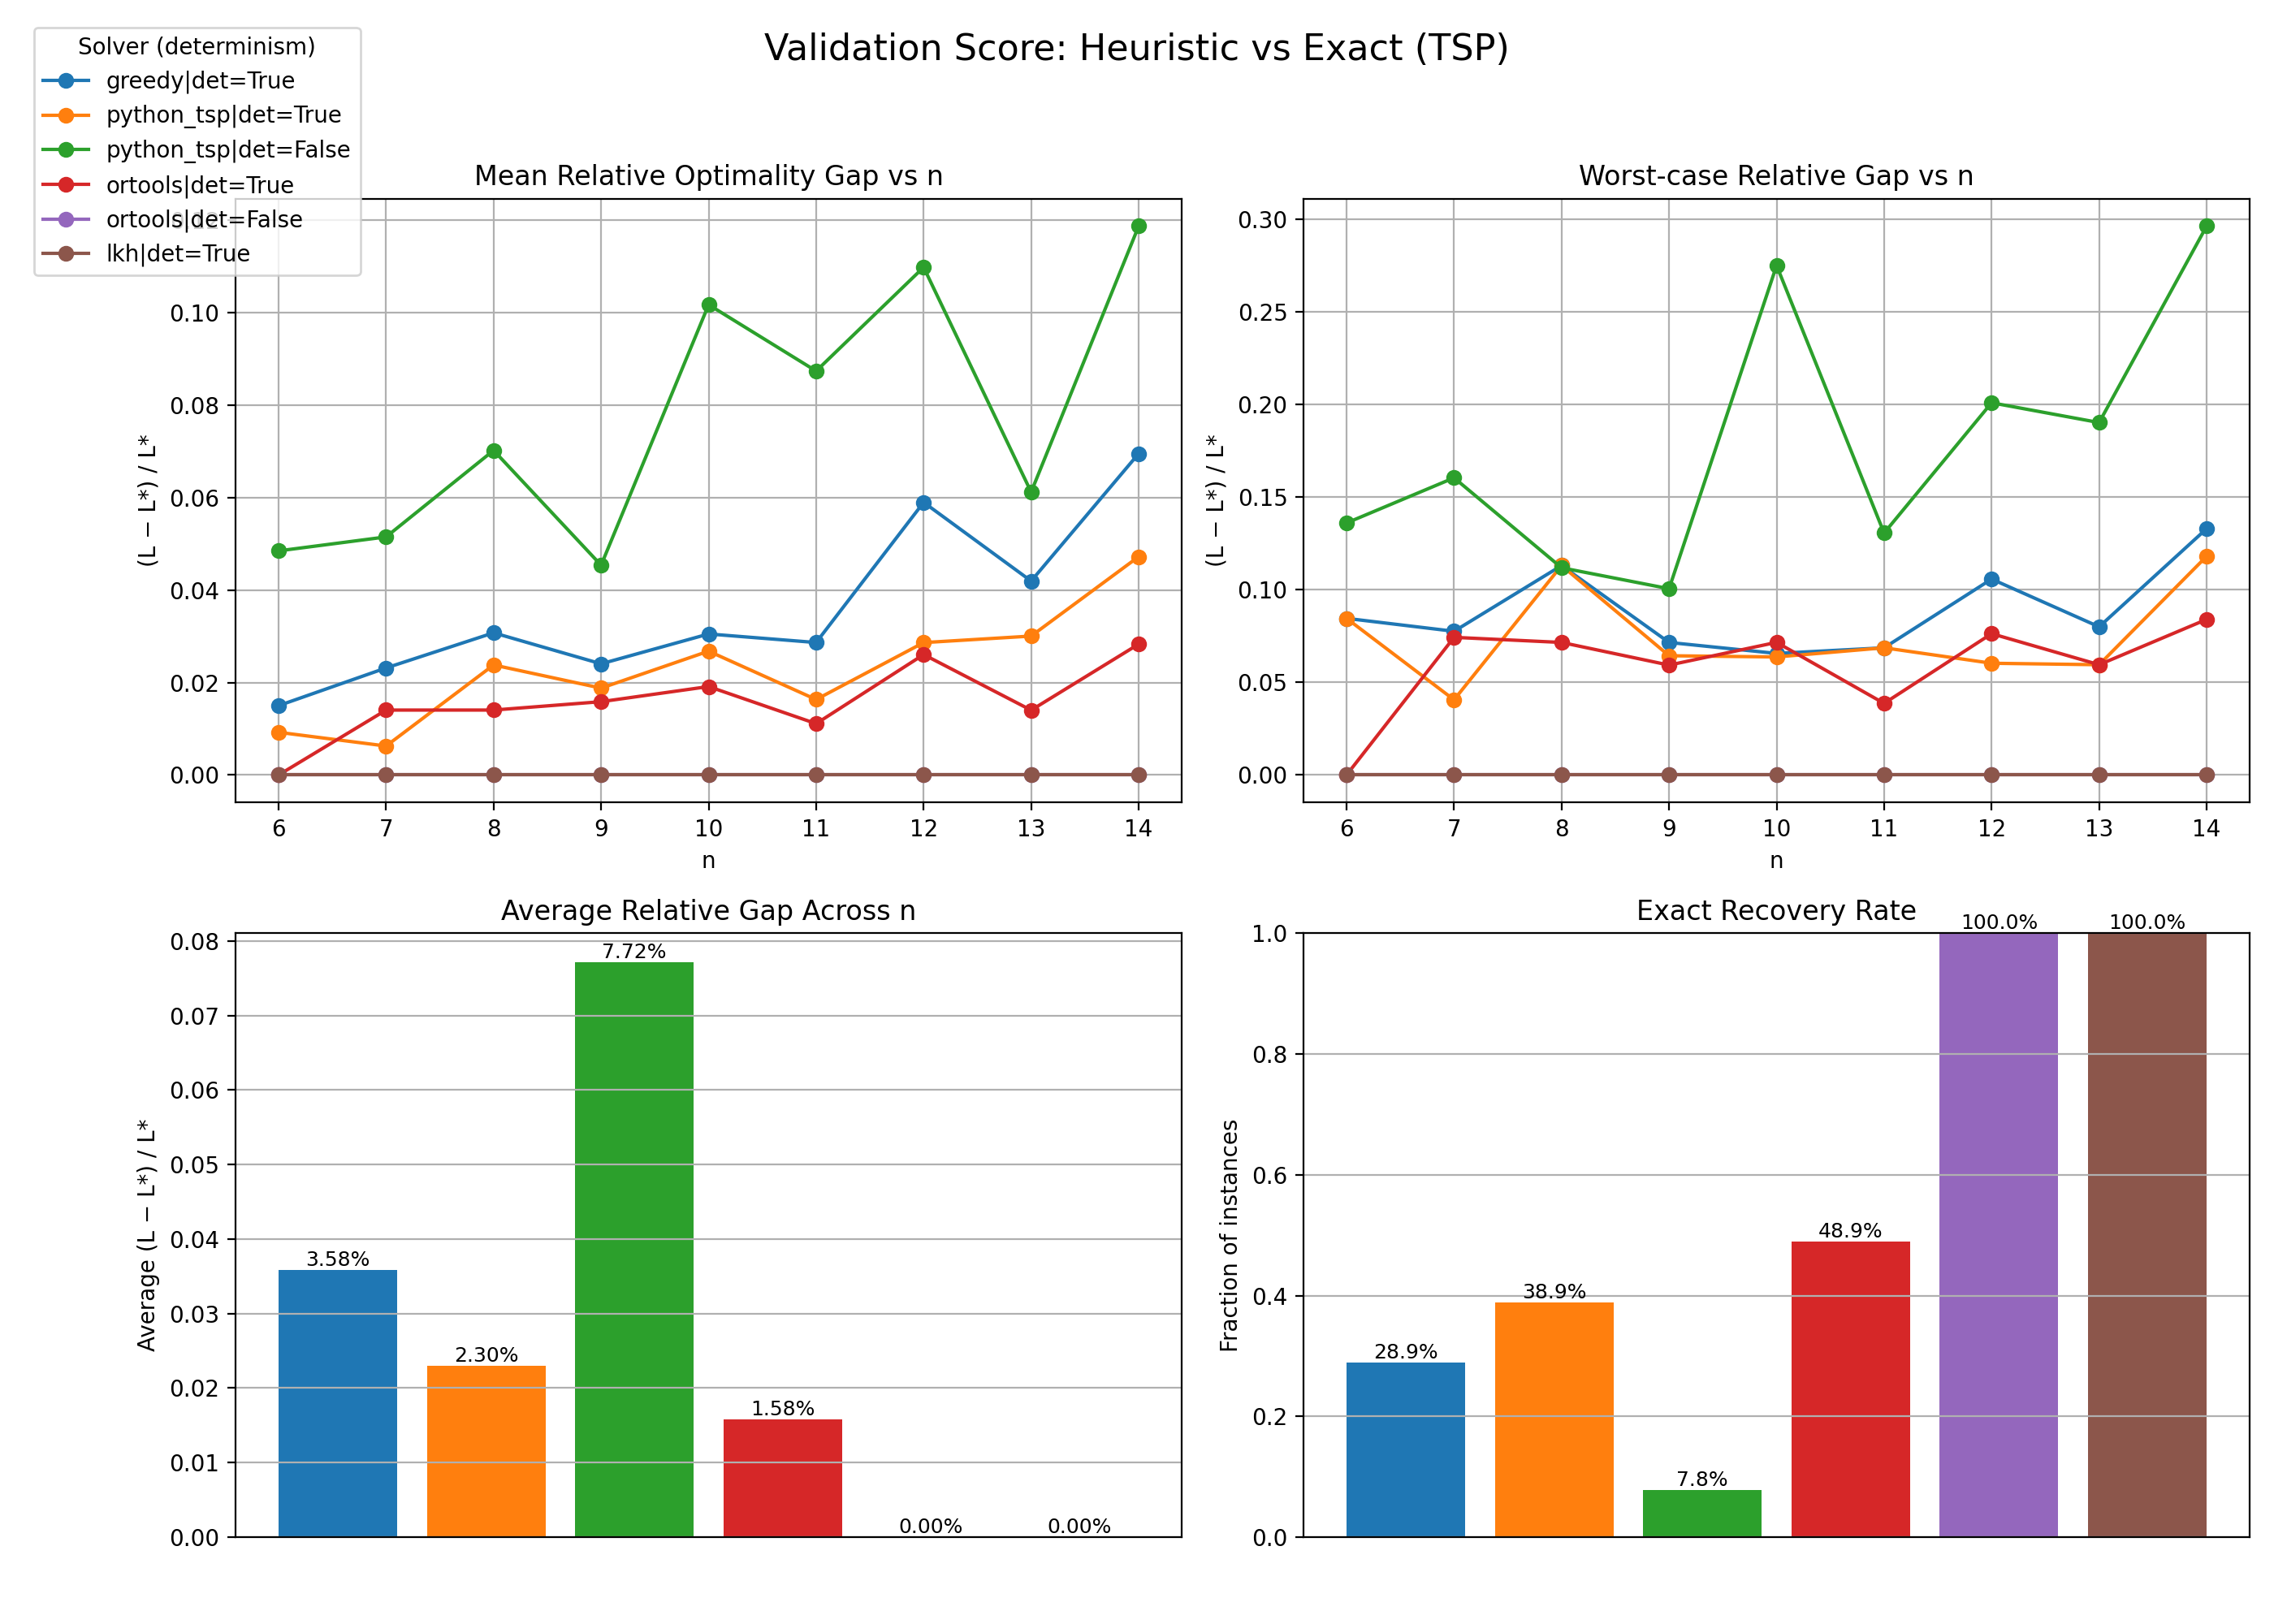
\includegraphics[width=0.49\textwidth]{../../libraries/simulations/_img/validation/solvers/tsp/validation_exact_vs_heuristic_tsp.png}
\hfill
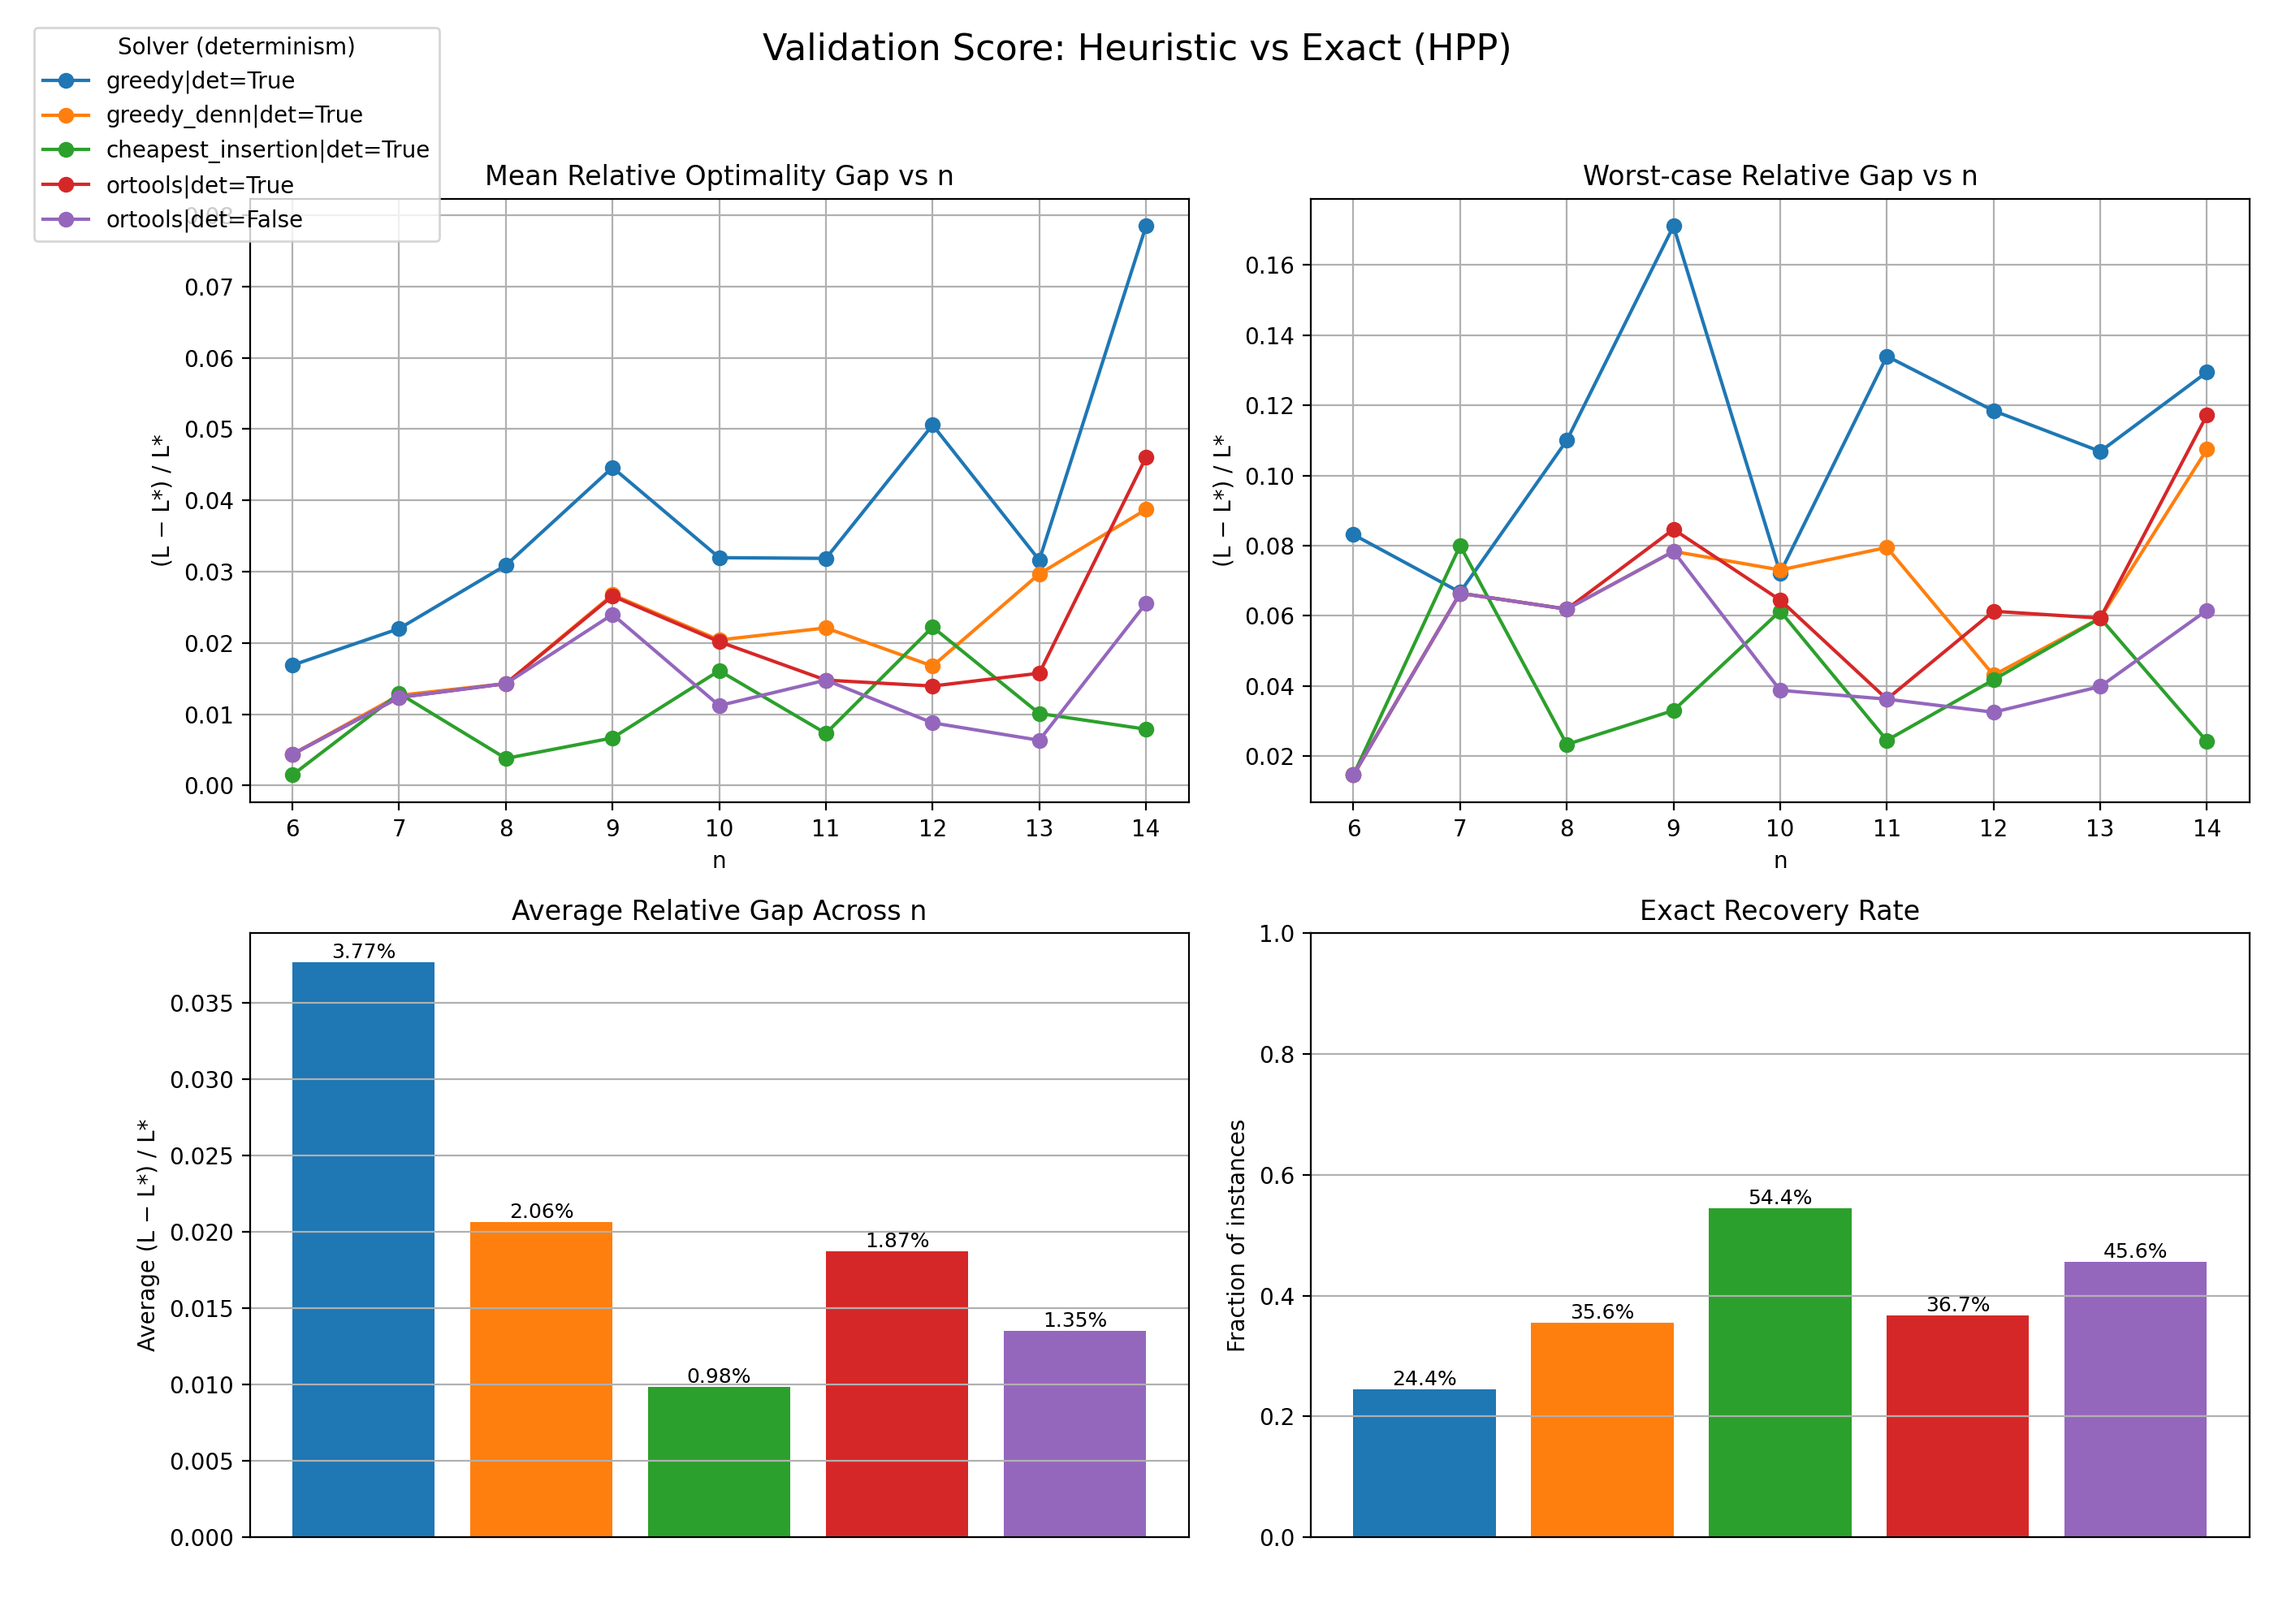
\includegraphics[width=0.49\textwidth]{../../libraries/simulations/_img/validation/solvers/hpp/validation_exact_vs_heuristic_hpp.png}
\caption{Route-solver validation against exact optimization for TSP (left) and HPP (right). The panels compare mean relative gap, worst-case relative gap, average relative gap, and exact recovery rate.}
\label{fig:solver-validation-main}
\end{figure}

\begin{table}[htbp]
\centering
\caption{Reading guide for the route-level exact-versus-heuristic validation.}
\label{tab:solver-validation-reading-guide}
\small
\renewcommand{\arraystretch}{1.18}
\begin{tabular}{@{}>{\raggedright\arraybackslash}p{0.13\textwidth}@{\hspace{0.8em}}>{\raggedright\arraybackslash}p{0.29\textwidth}@{\hspace{0.8em}}>{\raggedright\arraybackslash}p{0.25\textwidth}@{\hspace{0.8em}}>{\raggedright\arraybackslash}p{0.25\textwidth}@{}}
\toprule
Problem & Exact comparison & Strongest validation result & Interpretation \\
\midrule
TSP & Two solvers recover the exact optimum in all plotted cases. & \texttt{lkh} and non-deterministic \texttt{ortools}: $0.00\%$ gap, $100.0\%$ exact recovery. & TSP approximation can be exact in the validation range; later solver choice is mainly a runtime trade-off. \\
\addlinespace
HPP & No solver recovers the exact optimum in all plotted cases. & Best insertion heuristic: $0.98\%$ average gap, $54.4\%$ exact recovery. & HPP approximation is close, but route-level error must be tolerated and checked downstream. \\
\bottomrule
\end{tabular}
\par
\end{table}

\begin{table}[htbp]
\centering
\caption{Route-solver validation against exact optimization on simulated instances.}
\label{tab:solver-validation-summary}
\resizebox{\textwidth}{!}{%
\begin{tabular}{llccl}
\toprule
Problem type & Solver & Avg. relative gap & Exact recovery rate & Main interpretation \\
\midrule
TSP & \texttt{lkh} & $0.00\%$ & $100.0\%$ & Exact in all plotted validation cases. \\
TSP & \texttt{ortools} (\texttt{det=False}) & $0.00\%$ & $100.0\%$ & Exact in all plotted validation cases. \\
TSP & \texttt{ortools} (\texttt{det=True}) & $1.58\%$ & $48.9\%$ & Close to exact, but not exact recovery. \\
TSP & \texttt{python\_tsp} (\texttt{det=True}) & $2.30\%$ & $38.9\%$ & Moderate route-level loss. \\
TSP & \texttt{greedy} & $3.58\%$ & $28.9\%$ & Useful baseline, but weaker route quality. \\
TSP & \texttt{python\_tsp} (\texttt{det=False}) & $7.72\%$ & $7.8\%$ & Largest route-level deviation. \\
\midrule
HPP & \texttt{cheapest\_insertion} & $0.98\%$ & $54.4\%$ & Best average HPP approximation. \\
HPP & \texttt{ortools} (\texttt{det=False}) & $1.35\%$ & $45.6\%$ & Strong HPP approximation, but not exact. \\
HPP & \texttt{ortools} (\texttt{det=True}) & $1.87\%$ & $36.7\%$ & Acceptable route-level approximation. \\
HPP & \texttt{greedy\_denn} & $2.06\%$ & $35.6\%$ & Fast, but less accurate. \\
HPP & \texttt{greedy} & $3.77\%$ & $24.4\%$ & Weakest HPP approximation. \\
\bottomrule
\end{tabular}
\par}
\end{table}

\subsubsection{Outlier-Level Agreement With Exhaustive Detection}

The second validation layer evaluates whether approximate candidate search preserves the exact economic diagnosis. Here the exact reference is the exhaustive outlier detector: every non-empty candidate subset is evaluated, and the resulting best subset, optimized route length, and maximum marginal effect define the benchmark. The approximate methods are then scored against this exact result.

The panels in Appendix~\ref{app:validation-figures} show a consistent pattern. Plain candidate search is often close to the exact diagnosis, but it has visible failure cases. Method set \texttt{A} improves the approximation substantially. Method set \texttt{B} alone is less reliable, especially in the TSP panels where it can collapse at the largest plotted instance size. The most stable approximation is obtained when beam expansion is included. \texttt{Beam}, \texttt{A+Beam}, \texttt{B+Beam}, and \texttt{A+B+Beam} generally keep the average agreement scores at or very near one.

\begin{table}[htbp]
\centering
\caption{Condensed summary of outlier-validation performance relative to exact evaluation.}
\label{tab:outlier-validation-summary}
\resizebox{\textwidth}{!}{%
\begin{tabular}{llccc}
\toprule
Setting & Method set & Avg. Jaccard & Avg. $L_{\mathrm{opt}}$ agreement & Avg. $C_2^{\max}$ agreement \\
\midrule
TSP Type 1 & plain & 0.822 & 0.842 & 0.847 \\
TSP Type 1 & \texttt{A} & 0.953 & 0.958 & 0.992 \\
TSP Type 1 & \texttt{A+B} & 0.953 & 0.958 & 0.992 \\
TSP Type 1 & \texttt{Beam} & 1.000 & 1.000 & 1.000 \\
TSP Type 1 & \texttt{A+Beam} & 0.994 & 0.996 & 0.998 \\
\midrule
TSP Type 2 (\texttt{ortools}, det.) & plain & 0.833 & 0.834 & 0.836 \\
TSP Type 2 (\texttt{ortools}, det.) & \texttt{A} & 0.992 & 0.986 & 0.993 \\
TSP Type 2 (\texttt{ortools}, det.) & \texttt{A+B} & 1.000 & 0.998 & 0.995 \\
TSP Type 2 (\texttt{ortools}, det.) & \texttt{Beam} & 1.000 & 0.998 & 0.995 \\
TSP Type 2 (\texttt{ortools}, det.) & \texttt{A+Beam} & 1.000 & 0.998 & 0.995 \\
\midrule
TSP Type 2 (\texttt{lkh}) & plain & 0.833 & 0.835 & 0.839 \\
TSP Type 2 (\texttt{lkh}) & \texttt{A} & 0.983 & 0.976 & 0.997 \\
TSP Type 2 (\texttt{lkh}) & \texttt{A+B} & 0.992 & 0.989 & 0.999 \\
TSP Type 2 (\texttt{lkh}) & \texttt{Beam} & 1.000 & 1.000 & 1.000 \\
TSP Type 2 (\texttt{lkh}) & \texttt{A+Beam} & 1.000 & 1.000 & 1.000 \\
\midrule
HPP Type 1 & plain & 0.917 & 0.933 & 0.928 \\
HPP Type 1 & \texttt{A} & 0.967 & 0.969 & 0.978 \\
HPP Type 1 & \texttt{A+B} & 0.967 & 0.969 & 0.978 \\
HPP Type 1 & \texttt{Beam} & 1.000 & 1.000 & 1.000 \\
HPP Type 1 & \texttt{A+Beam} & 1.000 & 1.000 & 1.000 \\
\midrule
HPP Type 2 (\texttt{ortools}, det.) & plain & 0.983 & 0.983 & 0.977 \\
HPP Type 2 (\texttt{ortools}, det.) & \texttt{A} & 1.000 & 0.995 & 0.993 \\
HPP Type 2 (\texttt{ortools}, det.) & \texttt{A+B} & 1.000 & 0.995 & 0.993 \\
HPP Type 2 (\texttt{ortools}, det.) & \texttt{Beam} & 1.000 & 0.995 & 0.993 \\
HPP Type 2 (\texttt{ortools}, det.) & \texttt{A+Beam} & 1.000 & 0.995 & 0.993 \\
\midrule
HPP Type 2 (\texttt{cheapest\_insertion}) & plain & 0.983 & 0.984 & 0.973 \\
HPP Type 2 (\texttt{cheapest\_insertion}) & \texttt{A} & 1.000 & 0.997 & 0.990 \\
HPP Type 2 (\texttt{cheapest\_insertion}) & \texttt{A+B} & 1.000 & 0.997 & 0.990 \\
HPP Type 2 (\texttt{cheapest\_insertion}) & \texttt{Beam} & 1.000 & 0.997 & 0.990 \\
HPP Type 2 (\texttt{cheapest\_insertion}) & \texttt{A+Beam} & 1.000 & 0.997 & 0.990 \\
\bottomrule
\end{tabular}
\par}
\end{table}

Table~\ref{tab:outlier-validation-summary} condenses the main results against the exact reference. TSP Type~1 illustrates the gain from candidate expansion: the plain method attains an average Jaccard agreement of $0.822$ and $C_2^{\max}$ agreement of $0.847$, while \texttt{Beam} reaches $1.000$ on all three reported metrics. TSP Type~2 shows the same structure. With deterministic \texttt{ortools}, the plain method averages $0.833$ Jaccard agreement and $0.836$ agreement in $C_2^{\max}$, whereas the beam-based variants are at $0.995$--$1.000$ on the reported metrics. With \texttt{lkh}, the beam-based variants recover the exact Type~2 diagnosis completely in the summarized averages.

The HPP panels are more forgiving at the outlier-diagnosis level than the route-level validation alone might suggest. Even though HPP route solvers do not always recover the exact optimized path, the resulting economic outlier diagnosis remains highly stable. For HPP Type~2 with deterministic \texttt{ortools}, the plain method already reaches $0.983$ Jaccard agreement and $0.977$ agreement in $C_2^{\max}$, while the expanded methods reach $1.000$ Jaccard agreement and approximately $0.993$ agreement in $C_2^{\max}$. With \texttt{cheapest\_insertion}, the corresponding expanded methods reach $1.000$ Jaccard agreement and approximately $0.990$ agreement in $C_2^{\max}$. Thus, the exact benchmark shows that modest HPP route-length error does not necessarily translate into materially different outlier classification.

\begin{table}[htbp]
\centering
\caption{Main validation conclusions relative to exact reference results.}
\label{tab:validation-conclusions}
\small
\renewcommand{\arraystretch}{1.18}
\begin{tabular}{@{}>{\raggedright\arraybackslash}p{0.20\textwidth}@{\hspace{1em}}>{\raggedright\arraybackslash}p{0.36\textwidth}@{\hspace{1em}}>{\raggedright\arraybackslash}p{0.36\textwidth}@{}}
\toprule
Conclusion & Exact-reference evidence & Implication for the analysis \\
\midrule
\textbf{TSP can match the exact optimum.} & \texttt{lkh} and non-deterministic \texttt{ortools} both show $0.00\%$ average gap and $100.0\%$ exact recovery. & Exact-quality TSP route solving is available in the validation range. Solver choice can therefore be evaluated mainly as a quality--runtime trade-off. \\
\addlinespace
\textbf{HPP is close, but not exact.} & The best HPP average gap is $0.98\%$ for \texttt{cheapest\_insertion}; no HPP solver reaches $100.0\%$ exact recovery. & Open-path results should be interpreted as close approximations rather than exact reproductions. \\
\addlinespace
\textbf{Beam expansion is essential.} & Beam-based method sets typically score near $1.000$ on Jaccard, $L_{\mathrm{opt}}$, and $C_2^{\max}$ agreement. & Candidate reduction is acceptable when it retains beam expansion, not when it relies only on simple screens. \\
\addlinespace
\textbf{Diagnostic stability matters most.} & HPP Type~2 remains stable at the outlier level even when route recovery is incomplete. & The decisive validation criterion is preservation of the economic outlier diagnosis, not route length alone. \\
\bottomrule
\end{tabular}
\par
\end{table}

Taken together, the exact comparisons support the use of approximation in the remainder of the article, but with two qualifications. First, exact route solving is not replaced because it is unimportant; it is replaced because it becomes computationally infeasible at the scale of the substantive analysis. Second, approximation is only defensible because the validation checks the final economic diagnosis against exact results where exact results are still available. The evidence indicates that carefully chosen route heuristics, combined with beam-based candidate expansion, preserve the relevant outlier conclusions closely enough to proceed to larger operational routes.

\subsection{Route Solver Selection}
\label{subsec:route-solver-selection}

The route solver is an internal component of Type~2 rather than the object of analysis in itself. It affects the optimized route terms $L^*(R)$ and $L^*(R\setminus S)$, and these values subsequently enter the economic effect $C_2^*(S)$. Solver selection therefore requires two checks: whether the solver produces sufficiently strong routes at acceptable cost, and whether remaining route differences materially change the downstream economic diagnosis.

\subsubsection{Direct Solver Benchmarks}

The direct benchmarks show that the shortest route is not always the most useful computational choice. Tables~\ref{tab:tsp-direct-solver-benchmark} and~\ref{tab:hpp-direct-solver-benchmark} summarize the route-length and runtime trade-offs for TSP and HPP separately.

\begin{table}[htbp]
\centering
\caption{Direct TSP solver benchmark. Values are averages across the evaluated simulated instances.}
\label{tab:tsp-direct-solver-benchmark}
\resizebox{\textwidth}{!}{%
\begin{tabular}{lccp{5.8cm}}
\toprule
Solver configuration & Avg. tour length & Avg. runtime (s) & Interpretation \\
\midrule
\texttt{lkh} & 909.53 & 0.3808 & Shortest average tours, but slower than deterministic \texttt{ortools}. \\
\texttt{ortools} (\texttt{det=False}) & 945.11 & 2.0017 & Strong route quality, but runtime is governed by the two-second limit. \\
\texttt{ortools} (\texttt{det=True}) & 973.80 & 0.1669 & Good route quality with substantially lower runtime. \\
\texttt{python\_tsp} (\texttt{det=True}) & 1038.20 & 0.1666 & Similar runtime to deterministic \texttt{ortools}, but weaker routes. \\
\texttt{greedy} & 1060.31 & 0.0872 & Fastest, but route quality is weaker. \\
\texttt{python\_tsp} (\texttt{det=False}) & 1540.12 & 0.2291 & Weakest route quality in this benchmark. \\
\bottomrule
\end{tabular}
\par}
\end{table}

\begin{table}[htbp]
\centering
\caption{Direct HPP solver benchmark. Values are averages across the evaluated simulated instances.}
\label{tab:hpp-direct-solver-benchmark}
\resizebox{\textwidth}{!}{%
\begin{tabular}{lccp{5.8cm}}
\toprule
Solver configuration & Avg. path length & Avg. runtime (s) & Interpretation \\
\midrule
\texttt{ortools} (\texttt{det=False}) & 896.25 & 2.0613 & Shortest average paths, but expensive for repeated Type~2 evaluation. \\
\texttt{cheapest\_insertion} & 912.74 & 2.6773 & Strong path quality, but the slowest direct HPP solver. \\
\texttt{ortools} (\texttt{det=True}) & 929.88 & 0.2210 & Slightly longer paths, but much lower runtime. \\
\texttt{greedy\_denn} & 962.08 & 0.0597 & Very fast, but path quality is weaker. \\
\texttt{greedy} & 994.08 & 0.0539 & Fastest, but weakest path quality among the tested HPP solvers. \\
\bottomrule
\end{tabular}
\par}
\end{table}

For TSP, \texttt{lkh} gives the strongest direct route quality, but deterministic \texttt{ortools} gives a better practical balance. For HPP, the strongest path-quality variants are slower. This matters because Type~2 repeatedly solves modified routes during candidate subset evaluation.

\subsubsection{HPP Initial-Point Selection}

The HPP case requires an additional choice because an open Hamiltonian path must also commit to endpoints. The initial-point study in Figure~\ref{fig:hpp-initial-point-study} compares deterministic and non-deterministic \texttt{ortools} configurations. The compact summary in Table~\ref{tab:hpp-initial-point-summary} shows that deterministic \texttt{GREEDY} initialization gives the strongest deterministic path quality while remaining far below the runtime of the non-deterministic alternatives.

\begin{figure}[htbp]
\centering
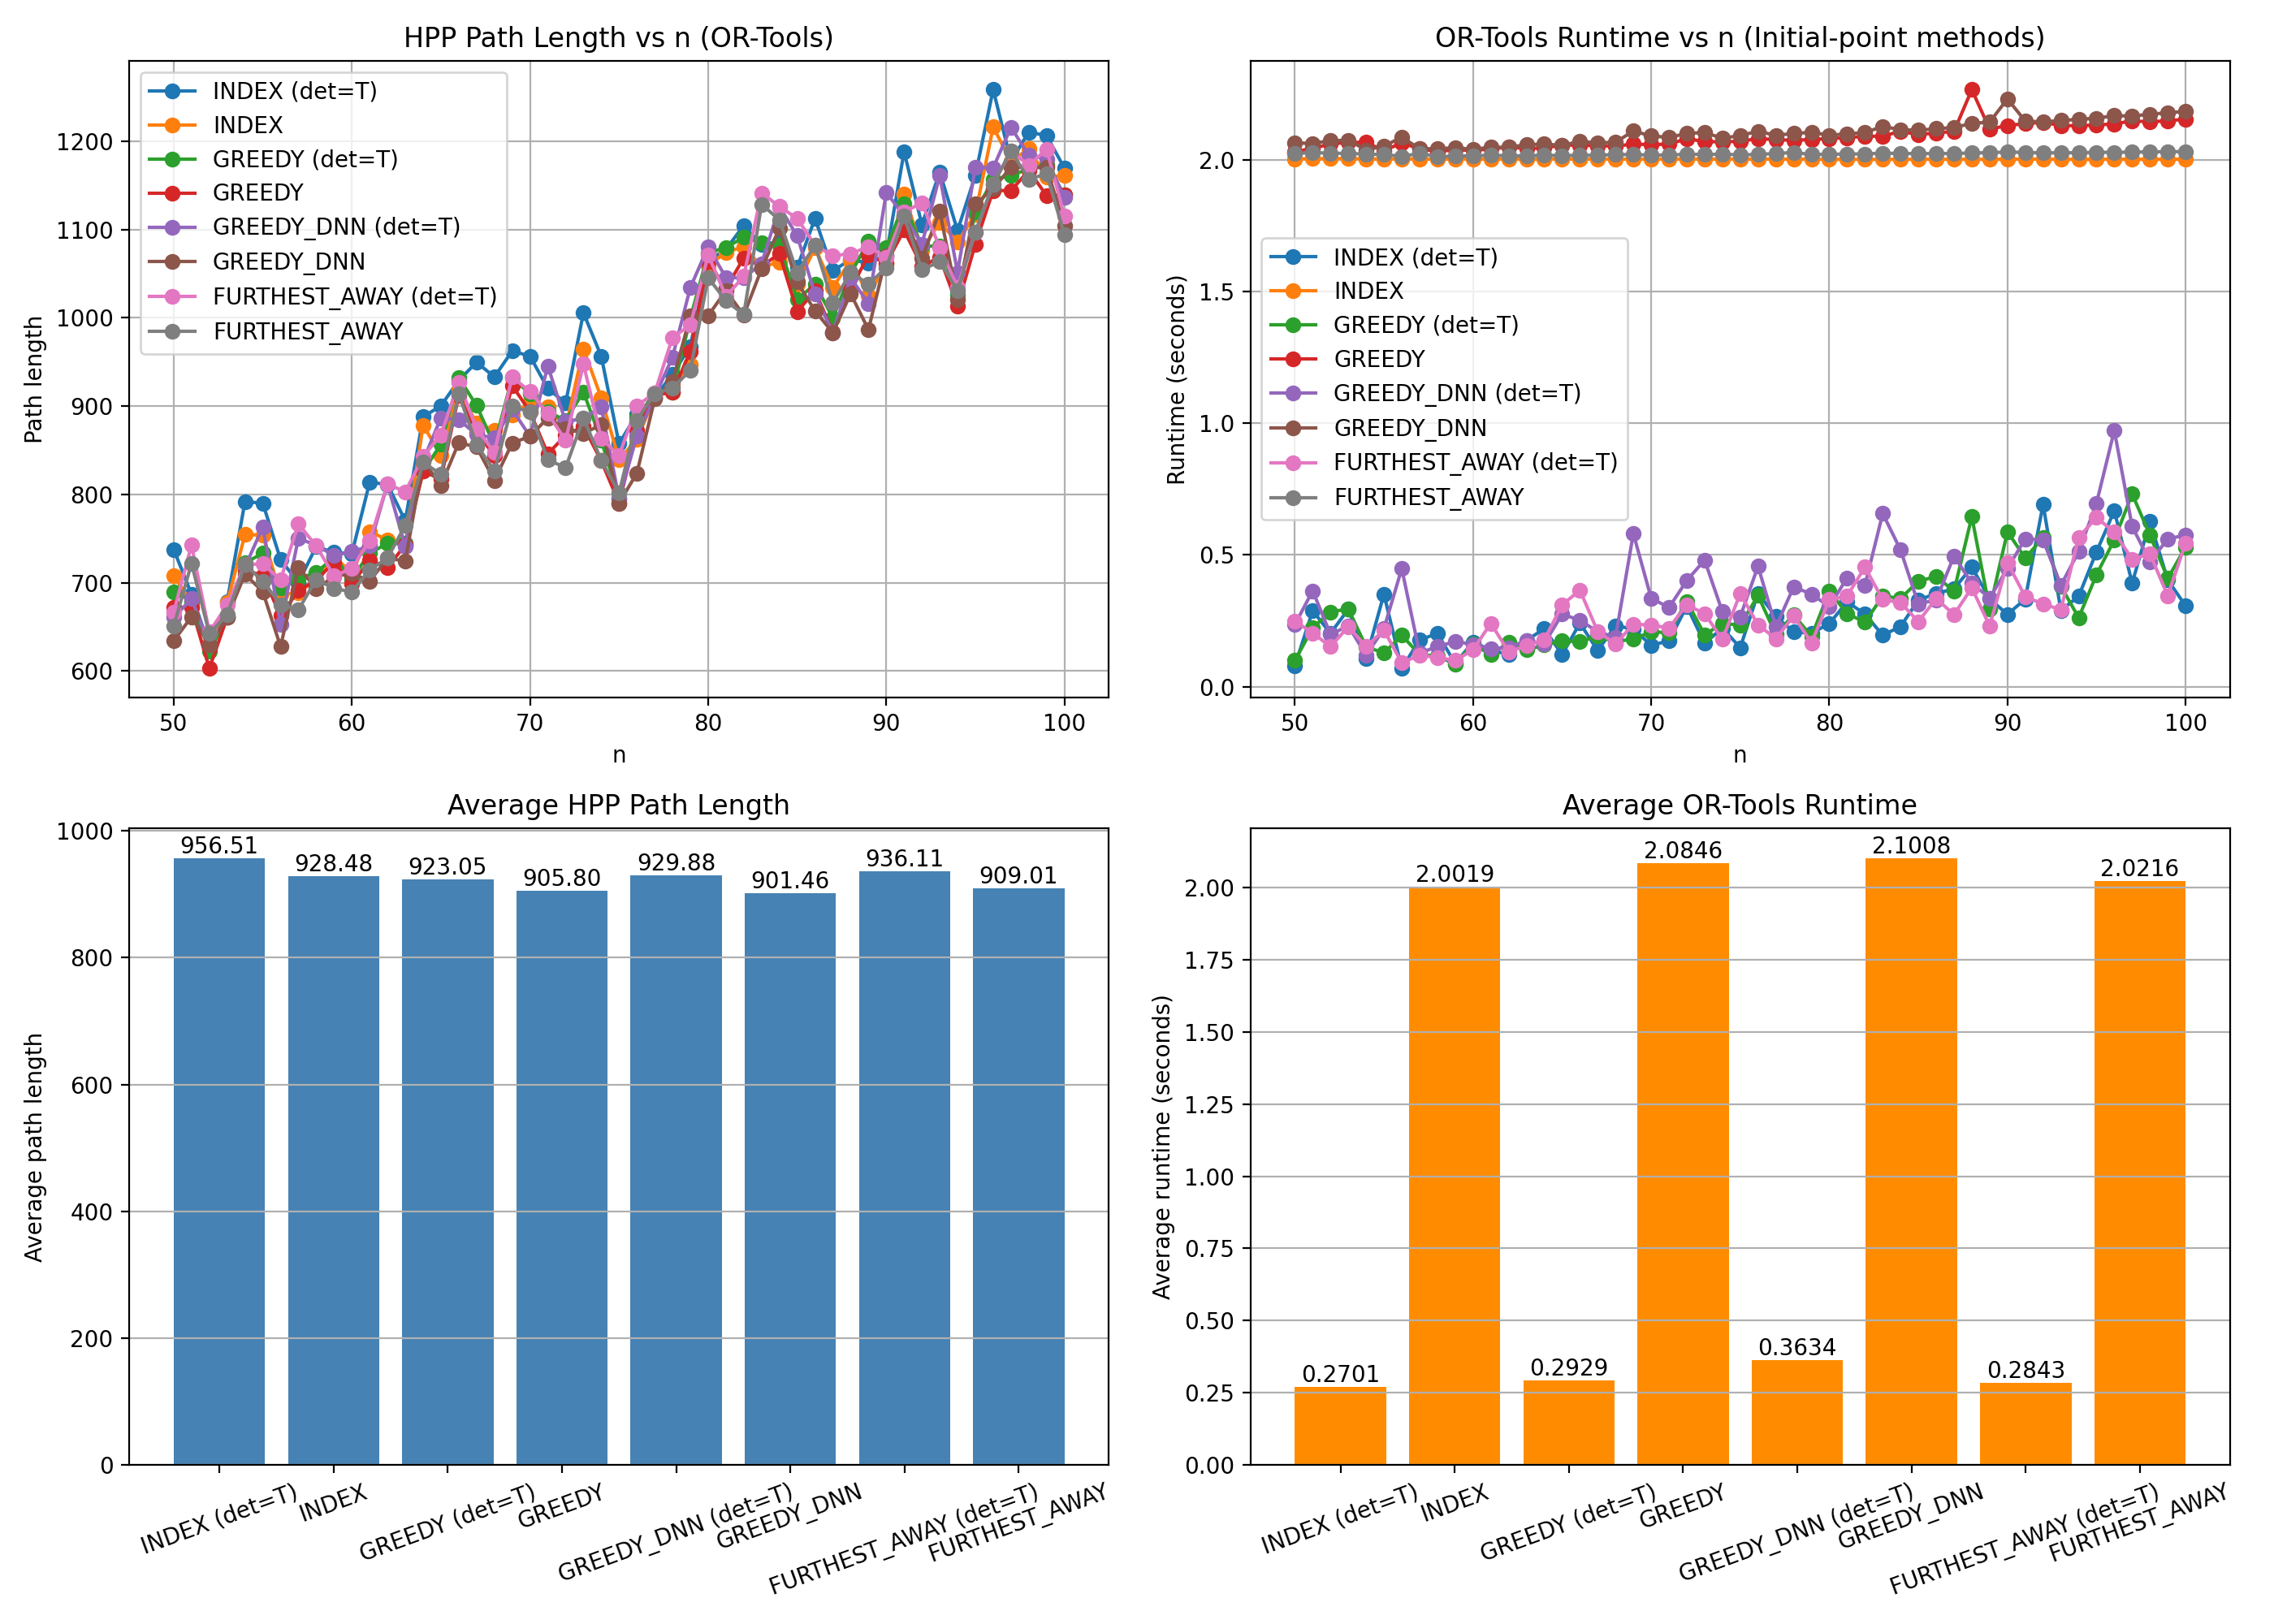
\includegraphics[width=\textwidth]{../../libraries/simulations/_img/benchmarks/hpp/hpp_initial_point_study.png}
\caption{HPP initial-point benchmark for \texttt{ortools}. The figure compares path length and runtime across endpoint-initialization strategies.}
\label{fig:hpp-initial-point-study}
\end{figure}

\begin{table}[htbp]
\centering
\caption{Selected HPP initial-point results for \texttt{ortools}.}
\label{tab:hpp-initial-point-summary}
\resizebox{\textwidth}{!}{%
\begin{tabular}{lccp{5.8cm}}
\toprule
Initial-point configuration & Avg. path length & Avg. runtime (s) & Interpretation \\
\midrule
\texttt{GREEDY} (\texttt{det=True}) & 923.05 & 0.2929 & Best deterministic path length. \\
\texttt{FURTHEST\_AWAY} (\texttt{det=True}) & 936.11 & 0.2843 & Similar runtime, weaker path quality. \\
\texttt{INDEX} (\texttt{det=True}) & 956.51 & 0.2701 & Fast, but weakest deterministic path quality. \\
\texttt{GREEDY} (\texttt{det=False}) & 905.80 & 2.0846 & Stronger path quality, but substantially slower. \\
\texttt{GREEDY\_DNN} (\texttt{det=False}) & 901.46 & 2.1008 & Shortest reported paths, but not attractive for repeated use. \\
\bottomrule
\end{tabular}
\par}
\end{table}

\subsubsection{Downstream Economic Stability}

The direct route benchmarks do not by themselves determine the final solver. The downstream question is whether differences in route construction propagate into materially different optimized route lengths, margin gains, outlier counts, or runtimes once the full hybrid route-level analysis is applied. Table~\ref{tab:solver-downstream-benchmark} summarizes the selection-relevant averages, while the full route-by-route panels are reported in Appendix~\ref{app:hybrid-benchmark-figures}.

\begin{table}[htbp]
\centering
\caption{Route-level hybrid benchmark summary. Values are averages across the evaluated routes.}
\label{tab:solver-downstream-benchmark}
\resizebox{\textwidth}{!}{%
\begin{tabular}{llrrrrr}
\toprule
Problem & Method & Avg. $L^*$ & Avg. optimized gain & Avg. outliers & Avg. $\Delta$ gain & Avg. runtime (s) \\
\midrule
TSP & Type~1 baseline & 3702 & 541 & 1 & 6 & 1 \\
TSP & Type~2 \texttt{greedy} & 2887 & 564 & 1 & 5 & 47 \\
TSP & Type~2 \texttt{python\_tsp} (\texttt{det=True}) & 2733 & 569 & 1 & 4 & 120 \\
TSP & Type~2 \texttt{python\_tsp} (\texttt{det=False}) & 3195 & 565 & 1 & 12 & 144 \\
TSP & Type~2 \texttt{ortools} (\texttt{det=True}) & 2772 & 569 & 1 & 3 & 35 \\
TSP & Type~2 \texttt{ortools} (\texttt{det=False}) & 2775 & 570 & 1 & 3 & 345 \\
TSP & Type~2 \texttt{lkh} & 2764 & 571 & 0 & 3 & 269 \\
\midrule
HPP & Type~1 baseline & 4667 & 279 & 2 & 23 & 1 \\
HPP & Type~2 \texttt{greedy} & 3873 & 304 & 6 & 63 & 29 \\
HPP & Type~2 \texttt{greedy\_denn} & 3723 & 311 & 6 & 62 & 31 \\
HPP & Type~2 \texttt{ortools} (\texttt{det=True}) & 4257 & 301 & 2 & 23 & 48 \\
HPP & Type~2 \texttt{ortools} (\texttt{det=False}) & 4237 & 302 & 2 & 22 & 345 \\
\bottomrule
\end{tabular}
\par}
\end{table}

The route-level panels sharpen the solver-selection argument. For TSP, deterministic \texttt{ortools} gives nearly the same average optimized gain as non-deterministic \texttt{ortools} and \texttt{lkh} (569 compared with 570 and 571), while reducing average runtime from 345 and 269 seconds to 35 seconds. Its average optimized route length is also close to the strongest TSP alternatives. For HPP, the greedy path heuristics produce larger average optimized gains and more identified outliers, but the OR-Tools comparison remains important for reproducibility: deterministic \texttt{ortools} gives almost the same optimized gain as the non-deterministic configuration (301 compared with 302) at a much lower runtime (48 seconds compared with 345 seconds). This makes the final HPP choice deliberately conservative: it prioritizes deterministic and stable route optimization over the larger outlier counts produced by simpler greedy path heuristics.

\subsubsection{Selected Configuration}

The final configuration is therefore chosen by combining route quality, runtime, reproducibility, and downstream economic stability. Table~\ref{tab:solver-final-selection} states the resulting selection.

\begin{table}[htbp]
\centering
\caption{Final route-solver configuration used in the subsequent empirical analysis.}
\label{tab:solver-final-selection}
\resizebox{\textwidth}{!}{%
\begin{tabular}{lll}
\toprule
Problem & Selected configuration & Rationale \\
\midrule
TSP & \texttt{ortools} (\texttt{det=True}) & Retains similar downstream economic results to stronger route solvers at substantially lower runtime. \\
HPP & \texttt{ortools} (\texttt{det=True}), \texttt{GREEDY} initialization & Provides acceptable path quality, strong runtime behavior, and stable downstream economic results. \\
\bottomrule
\end{tabular}
\par}
\end{table}

This selection does not imply that deterministic \texttt{ortools} is the shortest-route solver in every benchmark. Rather, within the evaluated instances it provides the most appropriate operational balance for repeated Type~2 evaluation. With the route-solver configuration fixed, the analysis can turn to the substantive question of how often economic outliers occur in real operational routes.

\subsection*{Data Basis for the Real-Route Analysis}

The real-route analysis is based on an operational route dataset that combines route structure, route-unit coordinates, transport mode, routing problem type, and address-level revenue information. The route records are joined with weekly revenue observations and transformed into a route-profile table with one observation per route, cost profile, revenue profile, routing problem, and outlier definition. The first real-route analyses focus on addresses with revenue in at least one of the observed weeks and use the average-revenue profile together with the O18 distributor cost profile. This profile represents the normal adult distributor wage assumption used as the baseline in the main empirical analysis.

The first empirical analyses use a deliberately restricted scenario. Only revenue-generating addresses in the average-week profile are included, and the economic cost profile is fixed to \texttt{O18 Omdeler}. This APR profile represents the wage-cost assumptions for a standard distributor over 18 years old. The restriction keeps the prevalence results conditional on one revenue and cost setting, rather than mixing several economic scenarios in the same descriptive comparison.

\subsection{Prevalence of Economic Outliers}
\label{subsec:prevalence-of-economic-outliers}

After establishing methodological credibility and fixing the route-solver configuration, the analysis turns to the first substantive real-data question: how often economically inefficient route units occur in the operational data. The analysis in this subsection uses the \texttt{O18 Omdeler} APR profile and the \texttt{Gns. Oms} week profile. For each outlier definition, the filtered dataset contains 140 route profiles, consisting of 35 HPP profiles and 105 TSP profiles. Type~1 and Type~2 are reported separately because prevalence is conditional on the route reference under which economic harm is measured.

Table~\ref{tab:prevalence-route-status} shows that economic outliers are common at the route-profile level. Under the fixed-sequence definition, 115 of 140 route profiles contain at least one significant outlier, corresponding to 82.1\%. Under the optimized-sequence definition, the corresponding number is 114 profiles, or 81.4\%. Re-optimization therefore changes the share of affected route profiles only marginally in this filtered scenario.

\begin{table}[htbp]
\centering
\caption{Route profiles with and without significant economic outliers.}
\label{tab:prevalence-route-status}
\small
\begin{tabular}{llrr}
\toprule
Type & Outlier status & Route profiles & Share \\
\midrule
Type~1 & With outliers & 115 & 82.1\% \\
Type~1 & Without outliers & 25 & 17.9\% \\
Type~2 & With outliers & 114 & 81.4\% \\
Type~2 & Without outliers & 26 & 18.6\% \\
\bottomrule
\end{tabular}
\par
\end{table}

\begin{figure}[htbp]
\centering

\includegraphics[width=0.49\textwidth]{\detokenize{../analysis/_img/sektion 6.3/Number of significant outliers.png}}
\hfill

\includegraphics[width=0.49\textwidth]{\detokenize{../analysis/_img/sektion 6.3/Routes with and without significant outliers.png}}
\caption{Distribution of significant outliers per route profile (left) and the aggregate share of route profiles with and without significant outliers (right).}
\label{fig:prevalence-route-outliers}
\end{figure}

The distribution in Figure~\ref{fig:prevalence-route-outliers} adds two qualifications. First, all HPP profiles contain at least one significant outlier under both definitions, but Type~2 shifts the number of removed addresses downward. For HPP, the Type~1 distribution is concentrated at three and four outliers per profile, with shares of 42.9\% and 28.6\%, whereas Type~2 is concentrated at one and two outliers, each with a share of 40.0\%. Second, the profiles without outliers are found in the TSP group. For TSP, Type~1 has 23.8\% profiles with no outliers and substantial mass at one and three outliers; Type~2 increases the no-outlier share slightly to 24.8\% and concentrates 61.9\% of profiles at one or two outliers.

The route-profile prevalence should not be confused with the address-level scale of removal. Table~\ref{tab:prevalence-address-scale} shows that the selected outliers account for a small share of all addresses. In aggregate, Type~1 identifies 355 outlier addresses out of 15,959 addresses, or approximately 2.2\%. Type~2 identifies 218 outlier addresses, or approximately 1.4\%. Thus, the phenomenon is widespread across route profiles, but narrow within each route.

\begin{table}[htbp]
\centering
\caption{Address-level scale of significant economic outliers by problem type.}
\label{tab:prevalence-address-scale}
\resizebox{\textwidth}{!}{%
\begin{tabular}{llrrrrr}
\toprule
Type & Problem & Route profiles & Outlier addresses & Total addresses & Share of addresses & Mean removed share \\
\midrule
Type~1 & HPP & 35 & 126 & 3,644 & 3.5\% & 3.6\% \\
Type~1 & TSP & 105 & 229 & 12,315 & 1.9\% & 2.2\% \\
Type~2 & HPP & 35 & 68 & 3,644 & 1.9\% & 1.9\% \\
Type~2 & TSP & 105 & 150 & 12,315 & 1.2\% & 1.4\% \\
\bottomrule
\end{tabular}
\par}
\end{table}

The same pattern is visible in the distribution of removed-address shares in Figure~\ref{fig:prevalence-removal-scale}. Most route profiles have only a low single-digit percentage of addresses removed, especially under Type~2. The upper tail remains operationally relevant, but it is not representative of the typical route profile. This distinction is important for interpretation: economic outlier detection identifies a frequent diagnostic condition, not a large-scale pruning of the route network.

\begin{figure}[htbp]
\centering

\includegraphics[width=0.49\textwidth]{\detokenize{../analysis/_img/sektion 6.3/Share of addresses removed per route.png}}
\hfill

\includegraphics[width=0.49\textwidth]{\detokenize{../analysis/_img/sektion 6.3/ChangeOfRouteLengthDestribution.png}}
\caption{Share of addresses removed per route profile (left) and change in route length after outlier removal, measured as \textit{Length Opt} minus \textit{Length Org} (right).}
\label{fig:prevalence-removal-scale}
\end{figure}

Finally, the route-length distributions in Figure~\ref{fig:prevalence-removal-scale} are concentrated below zero. Since the plotted quantity is \textit{Length Opt} minus \textit{Length Org}, negative values indicate that the route becomes shorter after the selected outlier removal. The mass below zero confirms that the prevalence results are associated with modeled route-length reductions, while the density close to zero in the TSP panels shows that many removals are small in physical scale. Overall, Type~2 gives the stricter diagnosis in terms of intensity rather than incidence: it leaves the share of affected route profiles almost unchanged, but reduces the number and address share of selected outliers.

\subsection{Economic Impact of Outlier Removal}
\label{subsec:economic-impact-of-outlier-removal}

Prevalence alone does not establish whether the identified outliers are practically important. This subsection therefore asks what the modeled economic effect of removing the selected outlier subsets would be under the framework, measured through the change in contribution margin $\Delta DG = DG_{\text{after}} - DG_{\text{before}}$. The analysis examines absolute and relative contribution-margin improvement, average and median effects across routes, aggregate effects, revenue lost, route cost saved, route distance or time saved, and the number of route units removed. The central motivation is to make the trade-off between saved route cost and sacrificed revenue explicit, while interpreting these quantities as modeled improvement potentials rather than as observed causal profit gains from operational implementation.

The results show that the economic signal is positive in all combinations of route problem and outlier definition. Table~\ref{tab:economic-impact-summary} reports the aggregate revenue sacrificed, route cost saved, and resulting contribution-margin improvement. Type~1 produces a total modeled contribution-margin gain of $1{,}482.31$, while Type~2 produces a gain of $1{,}132.62$. The difference is expected, since Type~1 evaluates removals relative to the observed route sequence, whereas Type~2 first removes part of the route-order inefficiency through re-optimization. Type~1 therefore captures a broader fixed-sequence improvement potential; Type~2 gives the stricter optimized-sequence diagnosis.

\begin{table}[htbp]
\centering
\caption{Economic impact of removing the selected outlier subsets by route type and problem type.}
\label{tab:economic-impact-summary}
\resizebox{\textwidth}{!}{%
\begin{tabular}{llrrrrr}
\toprule
Outlier type & Problem & Revenue lost & Cost saved & $DG$ improvement & $DG$ improvement & Route-length saving \\
 &  &  &  &  & before--after & before--after \\
\midrule
Type~1 & HPP & 608.21 & 1,230.85 & 622.64 & 3.7\% & 16.0\% \\
Type~1 & TSP & 638.05 & 1,497.65 & 859.67 & 1.6\% & 11.0\% \\
Type~2 & HPP & 347.94 & 844.95 & 496.82 & 2.8\% & 11.9\% \\
Type~2 & TSP & 419.49 & 1,055.50 & 635.81 & 1.1\% & 9.2\% \\
\bottomrule
\end{tabular}
\par}
\end{table}

The positive contribution-margin effects arise because route cost savings exceed the associated revenue losses in each group. This relationship is visible directly in Figure~\ref{fig:economic-impact-tradeoff}: most observations lie on the favorable side of the cost-saving versus revenue-loss comparison, and the route-level economic change plots show negative revenue changes accompanied by larger negative cost changes. HPP routes have higher relative gains than TSP routes, particularly under Type~1, while TSP routes contribute more to the aggregate improvement because there are more TSP route profiles in the filtered data.

\begin{figure}[htbp]
\centering

\includegraphics[width=0.49\textwidth]{\detokenize{../analysis/_img/sektion 6.4/Removed outliers and economic change per route profile.png}}
\hfill

\includegraphics[width=0.49\textwidth]{\detokenize{../analysis/_img/sektion 6.4/Revenue lost versus cost saved.png}}
\caption{Route-level economic change by number of removed outliers (left) and revenue lost versus route cost saved (right).}
\label{fig:economic-impact-tradeoff}
\end{figure}

Figure~\ref{fig:economic-impact-relative-cumulative} further shows that the gains are not evenly distributed across routes. Relative improvements are concentrated close to zero for many route profiles, especially for TSP, but with a visible upper tail of economically meaningful cases. The cumulative curves also show that the total improvement is built from a limited number of positive route-level contributions rather than from uniformly large gains across the route population. Thus, economic outlier removal should be interpreted as a targeted correction mechanism: it frequently identifies affected route profiles, but most of the monetary improvement is concentrated in the subset of routes where the cost-revenue imbalance is strongest.

\begin{figure}[htbp]
\centering

\includegraphics[width=0.49\textwidth]{\detokenize{../analysis/_img/sektion 6.4/Relative DB improvement per route profile.png}}
\hfill

\includegraphics[width=0.49\textwidth]{\detokenize{../analysis/_img/sektion 6.4/Cumulative DB improvement by removed outliers.png}}
\caption{Relative contribution-margin improvement per route profile (left) and cumulative contribution-margin improvement from selected outlier removals (right).}
\label{fig:economic-impact-relative-cumulative}
\end{figure}

\subsection{Existing Route Efficiency}
\label{subsec:existing-route-efficiency}

Before interpreting the difference between Type~1 and Type~2, it is necessary to establish how efficiently the observed routes are already sequenced. This subsection therefore compares the observed route length $L(R)$ with the optimized route length $L^*(R)$ and evaluates the relative route gap implied by that difference. The motivation is theoretical as well as empirical: Type~1 evaluates economic harm relative to the current operating sequence, whereas Type~2 removes route-order inefficiency by re-optimizing the retained route. If the observed routes are already close to optimized, the two approaches may be expected to produce similar diagnoses; if not, route-sequence inefficiency may partly be attributed to individual route units under Type~1.

The Type~2 route benchmark indicates that the existing route sequences are not generally equal to the optimized reference. As shown in Table~\ref{tab:type2-route-efficiency-summary}, the original route is longer than the optimized route for 114 of the 140 route profiles, corresponding to 81.4\%. The pattern is strongest for HPP, where all 35 routes are longer than their optimized open-path reference. For TSP, 79 of 105 routes are longer than the optimized tour, while 26 routes are equal within tolerance. Across all route profiles, the optimized reference reduces route length or time by $58{,}573.5$, corresponding to 10.1\% of the original total.

\begin{table}[htbp]
\centering
\caption{Existing route efficiency under Type~2 optimization.}
\label{tab:type2-route-efficiency-summary}
\resizebox{\textwidth}{!}{%
\begin{tabular}{lrrrrrr}
\toprule
Problem & Route profiles & Original longer & Equal within tolerance & Total saving & Total saving & Mean saving \\
 &  &  &  &  & relative & relative \\
\midrule
All & 140 & 114 (81.4\%) & 26 (18.6\%) & 58,573.5 & 10.1\% & 9.1\% \\
HPP & 35 & 35 (100.0\%) & 0 (0.0\%) & 21,418.0 & 11.9\% & 12.0\% \\
TSP & 105 & 79 (75.2\%) & 26 (24.8\%) & 37,155.5 & 9.2\% & 8.2\% \\
\bottomrule
\end{tabular}
\par}
\end{table}

Figure~\ref{fig:route-efficiency-type2} illustrates both the route-efficiency gap and the relation between the two optimized reference lengths. HPP routes show consistently positive savings under Type~2 optimization, while TSP routes include a substantial mass close to zero and a smaller set of large positive savings. The comparison of Type~1 and Type~2 optimized lengths is concentrated around the diagonal, but with enough dispersion to matter for the economic diagnosis. This supports the need to distinguish between outliers that are harmful in the observed route and outliers that remain harmful after route-order inefficiency has been removed.

\begin{figure}[htbp]
\centering

\includegraphics[width=0.49\textwidth]{\detokenize{../analysis/_img/sektion 6.5/Existing route efficiency under Type 2 optimization.png}}
\hfill

\includegraphics[width=0.49\textwidth]{\detokenize{../analysis/_img/sektion 6.5/Type 1 optimized length versus Type 2 optimized length.png}}
\caption{Existing route efficiency under Type~2 optimization (left) and Type~1 optimized length versus Type~2 optimized length (right).}
\label{fig:route-efficiency-type2}
\end{figure}

The relation between Type~1 and Type~2 outlier sets confirms that the two definitions are related but not interchangeable. Table~\ref{tab:type1-type2-outlier-set-relations} classifies the set relation for the 140 route profiles. The most common case is that the Type~2 set is included in the Type~1 set, which occurs for 57 route profiles, or 40.7\%. A further 40 route profiles, corresponding to 28.6\%, have different non-nested sets. Exact equality, including both methods identifying no outliers, accounts for 35 profiles, or 25.0\%. Hence, the optimized-sequence diagnosis often narrows or changes the fixed-sequence diagnosis rather than simply reproducing it.

\begin{table}[htbp]
\centering
\caption{Relation between Type~1 and Type~2 outlier sets across route profiles.}
\label{tab:type1-type2-outlier-set-relations}
\small
\begin{tabular}{lrrr}
\toprule
Set relation & Routes & Share of routes & Mean Jaccard \\
\midrule
Both empty & 17 & 12.1\% & 1.000 \\
Equal non-empty & 18 & 12.9\% & 1.000 \\
Type~1 included in Type~2 & 8 & 5.7\% & 0.000 \\
Type~2 included in Type~1 & 57 & 40.7\% & 0.410 \\
Different non-nested & 40 & 28.6\% & 0.114 \\
\bottomrule
\end{tabular}
\par
\end{table}

Figure~\ref{fig:type1-type2-set-relations} adds the corresponding distributional view. HPP has no both-empty cases in this filtered sample, and disagreement is concentrated in Type~2-in-Type~1 and different-set cases. TSP contains more routes where both methods either agree on no outliers or agree exactly, but it also contains the only cases where the Type~1 set is included in the Type~2 set. The route-length saving distributions by set relation show why this distinction is material: disagreement between the two outlier definitions is connected to the amount of route-length improvement available under Type~2.

\begin{figure}[htbp]
\centering

\includegraphics[width=0.49\textwidth]{\detokenize{../analysis/_img/sektion 6.5/Relation between Type 1 and Type 2 outlier sets.png}}
\hfill

\includegraphics[width=0.49\textwidth]{\detokenize{../analysis/_img/sektion 6.5/Type 2 route-length saving by Type 1 and Type 2 outlier agreement.png}}
\caption{Relation between Type~1 and Type~2 outlier sets (left) and Type~2 route-length saving by outlier-set relation (right).}
\label{fig:type1-type2-set-relations}
\end{figure}

\subsection{Type 1 Versus Type 2 --- Robustness of the Economic Diagnosis}
\label{subsec:type-1-versus-type-2-robustness}

One of the central empirical questions of the article is whether route-sequence optimization materially changes which route units are identified as economic outliers. Type~1 asks whether a subset is economically harmful in the route as currently operated, while Type~2 asks whether the subset remains harmful after the retained route is arranged efficiently. This subsection therefore compares the two methods on the same routes under the same economic assumptions and classifies outcomes into categories such as no outliers under either method, Type~1 only, Type~2 only, and cases where both methods identify either the same or different subsets. The purpose is to distinguish sequence-dependent inefficiency from economic inefficiency that remains after the route-order effect has been removed, and to relate any disagreement to the route-efficiency gap documented in the previous subsection.

The comparison shows a consistent trade-off between intervention size and final route economics. On average, Type~2 sacrifices less revenue than Type~1, but it also saves less route cost. Table~\ref{tab:type1-type2-economic-comparison} reports the mean route-level differences. Relative to Type~1, Type~2 reduces the average revenue loss by $3.42$ and the average cost saving by $5.91$. The resulting contribution-margin improvement is therefore lower under Type~2 by $2.50$ per route profile, or 23.6\%. At the same time, the average contribution margin after removal is higher under Type~2 by $17.14$, reflecting the lower optimized route cost in the Type~2 reference structure.

\begin{table}[htbp]
\centering
\caption{Mean economic comparison between Type~1 and Type~2 at route-profile level.}
\label{tab:type1-type2-economic-comparison}
\resizebox{\textwidth}{!}{%
\begin{tabular}{lrrrr}
\toprule
Metric & Type~1 mean & Type~2 mean & Type~2 minus Type~1 & Relative difference \\
\midrule
Revenue lost & 8.90 & 5.48 & -3.42 & -38.4\% \\
Cost saved & 19.49 & 13.57 & -5.91 & -30.3\% \\
$DG$ improvement & 10.59 & 8.09 & -2.50 & -23.6\% \\
$DG$ after removal & 523.25 & 540.39 & 17.14 & 3.3\% \\
\bottomrule
\end{tabular}
\par}
\end{table}

The route-level comparison in Figure~\ref{fig:type1-versus-type2-db-improvement} shows that Type~1 more often produces the larger marginal improvement. This is also visible in Table~\ref{tab:type1-type2-db-improvement-comparison}: Type~1 gives the larger contribution-margin improvement for 65.7\% of HPP profiles and 55.2\% of TSP profiles, while Type~2 gives the larger improvement for 34.3\% and 23.8\%, respectively. For TSP, 21.0\% of profiles have the same improvement, mainly reflecting routes where neither method removes an outlier or where the selected change is economically neutral at the reported precision.

\begin{table}[htbp]
\centering
\caption{Which outlier definition gives the larger route-level contribution-margin improvement.}
\label{tab:type1-type2-db-improvement-comparison}
\small
\begin{tabular}{lrrr}
\toprule
Problem & Type~1 larger & Same & Type~2 larger \\
\midrule
HPP & 23 (65.7\%) & 0 (0.0\%) & 12 (34.3\%) \\
TSP & 58 (55.2\%) & 22 (21.0\%) & 25 (23.8\%) \\
\bottomrule
\end{tabular}
\par
\end{table}

\begin{figure}[htbp]
\centering

\includegraphics[width=0.49\textwidth]{\detokenize{../analysis/_img/sektion 6.6/Type 1 versus Type 2 DB improvement.png}}
\hfill

\includegraphics[width=0.49\textwidth]{\detokenize{../analysis/_img/sektion 6.6/Distribution of Type 2 minus Type 1 economic differences.png}}
\caption{Type~1 versus Type~2 contribution-margin improvement (left) and distribution of Type~2 minus Type~1 economic differences (right).}
\label{fig:type1-versus-type2-db-improvement}
\end{figure}

The distribution of Type~2 minus Type~1 differences clarifies the mechanism. Differences in revenue lost are mostly non-positive, meaning that Type~2 generally removes less revenue. Differences in cost saved are also mostly non-positive, meaning that the stricter optimized-sequence reference attributes less avoidable cost to the removed units. The contribution-margin improvement difference is therefore centered below zero: Type~2 is usually more conservative in the marginal gain it assigns to outlier removal, even though the final optimized route can have a higher contribution margin after removal.

Finally, Figure~\ref{fig:economic-differences-by-set-relation} shows that economic disagreement is structured by the relation between the selected outlier sets. When the Type~2 set is included in the Type~1 set, Type~2 typically removes less revenue and saves less cost, producing a smaller marginal improvement. When the Type~1 set is included in the Type~2 set, which occurs only for TSP in this filtered sample, the difference can move in the opposite direction. The empirical conclusion is therefore not that one definition dominates the other. Rather, the diagnosis is robust at the level of broad incidence, while the exact selected subset and the measured economic magnitude depend materially on whether current route sequencing is treated as part of the problem or removed through optimization.

\begin{figure}[htbp]
\centering

\includegraphics[width=0.74\textwidth]{\detokenize{../analysis/_img/sektion 6.6/Economic differences by Type 1 and Type 2 outlier-set relation.png}}
\caption{Economic differences between Type~2 and Type~1 by outlier-set relation.}
\label{fig:economic-differences-by-set-relation}
\end{figure}

\subsection{Characteristics of Routes with Economic Outliers}
\label{subsec:characteristics-of-routes-with-economic-outliers}

Having established where outliers occur and how they differ across route definitions, the next question is what kinds of routes tend to contain them. The purpose of this subsection is descriptive rather than predictive. Relevant route characteristics include route size, route length or time, total revenue, average revenue per route unit, contribution margin before removal, internal route-unit cost, and the route optimization gap. By comparing routes with identified outliers to routes without them, and where useful also separating Type~1-only, Type~2-only, both, and neither, the analysis seeks to clarify the operational contexts in which economic outlier problems are more likely to arise without interpreting simple associations as causal effects.

Table~\ref{tab:route-characteristics-outlier-presence} summarizes the main route-level differences in the focused data subset. Routes with outliers are not larger on average; they have fewer addresses than routes without outliers under both Type~1 and Type~2. The stronger distinction is route length. Under Type~1, routes with outliers have a mean route length of $4{,}993.33$, compared with $3{,}943.86$ for routes without outliers. Under Type~2, the corresponding means are $4{,}340.84$ and $3{,}339.49$. Mean revenue per address is very similar across the groups. The descriptive evidence therefore points more toward route structure and route extent than toward lower average address revenue as the immediate correlate of outlier presence.

\begin{table}[htbp]
\centering
\caption{Route characteristics with and without economic outliers.}
\label{tab:route-characteristics-outlier-presence}
\resizebox{\textwidth}{!}{%
\begin{tabular}{llrrrrrr}
\toprule
Outlier type & Outlier presence & Routes & Mean addresses & Median addresses & Mean route length & Mean revenue & Mean revenue per address \\
\midrule
Type~1 & With outliers & 115 & 111.80 & 110 & 4,993.33 & 653.50 & 5.84 \\
Type~1 & Without outliers & 25 & 124.08 & 126 & 3,943.86 & 715.05 & 5.77 \\
Type~2 & With outliers & 114 & 111.78 & 110 & 4,340.84 & 652.89 & 5.83 \\
Type~2 & Without outliers & 26 & 123.69 & 122 & 3,339.49 & 715.38 & 5.80 \\
\bottomrule
\end{tabular}
\par}
\end{table}

The transport-mode composition in Figure~\ref{fig:route-characteristics-main} gives a sharper operational interpretation. All 35 HPP car profiles contain outliers under both definitions. The routes without outliers occur only among TSP foot routes, where 80 of 105 profiles have Type~1 outliers and 79 of 105 have Type~2 outliers. This does not imply that car routes are intrinsically outlier-prone in general, since problem type and transport mode are confounded in the filtered sample. It does show, however, that within the observed real-route data the absence of economic outliers is concentrated in the foot-route segment.

\begin{figure}[htbp]
\centering

\includegraphics[width=0.49\textwidth]{\detokenize{../analysis/_img/sektion 6.7/Route characteristics with and without economic outliers.png}}
\hfill

\includegraphics[width=0.49\textwidth]{\detokenize{../analysis/_img/sektion 6.7/Route profiles with and without outliers by transport mode.png}}
\caption{Route characteristics by outlier presence (left) and route profiles with and without outliers by transport mode (right).}
\label{fig:route-characteristics-main}
\end{figure}

For HPP Type~1, the relative sequence position of selected outliers is informative because the open route has a directional structure. Figure~\ref{fig:route-characteristics-sequence-efficiency} shows that HPP Type~1 outliers are present throughout the route, but with a visible concentration toward the end of the sequence. In the underlying expanded outlier positions, 56 of 126 selected addresses, or 44.4\%, are located in the last 30\% of the original route, while 35 addresses, or 27.8\%, are in the first 30\%. This pattern is consistent with the open-path setting: late route units can impose substantial marginal continuation cost when evaluated under the observed sequence.

The route-efficiency gap also matters, but it is not a complete explanation. The scatter plot in Figure~\ref{fig:route-characteristics-sequence-efficiency} relates the Type~2 route-efficiency gap to the share of addresses flagged as outliers. Larger gaps are often associated with higher outlier shares, especially in the upper tail, but there are also routes with non-trivial efficiency gaps and low outlier prevalence. Economic outliers therefore appear where route structure, marginal travel cost, and local revenue interact; route inefficiency alone is insufficient to determine the diagnosis.

\begin{figure}[htbp]
\centering

\includegraphics[width=0.49\textwidth]{\detokenize{../analysis/_img/sektion 6.7/Relative sequence position of HPP Type 1 outliers.png}}
\hfill

\includegraphics[width=0.49\textwidth]{\detokenize{../analysis/_img/sektion 6.7/Route-efficiency gap versus outlier prevalence.png}}
\caption{Relative sequence position of HPP Type~1 outliers (left) and route-efficiency gap versus outlier prevalence (right).}
\label{fig:route-characteristics-sequence-efficiency}
\end{figure}

\subsection{Sensitivity to Economic Assumptions}
\label{subsec:sensitivity-to-economic-assumptions}

The final subsection asks how sensitive economic outlier identification is to alternative assumptions about revenue and route cost. Outlier status is not an intrinsic property of a route unit; it is conditional on the interaction between route structure, route-unit value, and service cost. Using the available revenue-profile and APR-profile combinations, the analysis therefore examines how the number of identified outliers, the share of routes containing outliers, the share of routes with no beneficial removal, the selected subsets, the contribution-margin improvement, and the agreement between Type~1 and Type~2 vary across economic scenarios. The purpose is to distinguish robust outliers, whose classification remains stable across plausible assumptions, from scenario-dependent outliers whose status changes when the economic environment changes.

The sensitivity analysis uses the predefined economic profiles applied throughout the empirical analysis. The APR profiles represent alternative unit-cost assumptions by transport mode. \textit{SE Omdeler} is the high-cost profile, based on a wage of 273 DKK per hour, with walking cost $0.0546$ DKK per meter, bicycle cost $0.01966$ DKK per meter, and car cost $0.07583$ DKK per second. \textit{O18 Omdeler} is the baseline adult-distributor profile used in Sections~6.3--6.7, based on 142 DKK per hour, with walking cost $0.0284$ DKK per meter, bicycle cost $0.01022$ DKK per meter, and car cost $0.03944$ DKK per second. \textit{U18 Omdeler} is the lower-cost under-18 profile, based on 81 DKK per hour, with walking cost $0.02009$ DKK per meter and bicycle cost $0.00624$ DKK per meter. The U18 profile is only evaluated for non-car route types in the scenario design; consequently, the HPP car sensitivity contains SE and O18, but not U18.

The revenue profiles represent alternative week assumptions from the same revenue source. \textit{Gns. Oms} uses the average revenue across weeks 2536--2539. The four observed week profiles \textit{U36}, \textit{U37}, \textit{U38}, and \textit{U39} use the corresponding individual weekly revenue fields. In the analysis below, APR sensitivity is evaluated at fixed revenue profile \textit{Gns. Oms}, while week-profile sensitivity is evaluated at fixed APR profile \textit{O18 Omdeler}. This separates cost sensitivity from revenue-week sensitivity.

Table~\ref{tab:apr-sensitivity-summary} shows the APR sensitivity. Higher route-cost assumptions systematically increase both the number of selected outliers and the modeled economic impact. For HPP car routes, both SE and O18 classify all 35 profiles as containing outliers, but the outlier rate falls from 5.7\% to 3.5\% under Type~1 and from 3.8\% to 1.9\% under Type~2 when moving from SE to O18. For TSP foot routes, the decline continues through U18: under Type~1, the share of routes with outliers falls from 92.4\% under SE to 76.2\% under O18 and 70.5\% under U18. The same ordered pattern appears for Type~2.

\begin{table}[htbp]
\centering
\caption{APR sensitivity at fixed revenue profile \textit{Gns. Oms}.}
\label{tab:apr-sensitivity-summary}
\resizebox{\textwidth}{!}{%
\begin{tabular}{lllrrrr}
\toprule
Route segment & APR profile & Outlier type & Routes with outliers & Outlier rate & Mean outliers & $DG$ improvement \\
\midrule
HPP / Car & SE Omdeler & Type~1 & 35 (100.0\%) & 5.7\% & 5.91 & 2,006.21 \\
HPP / Car & SE Omdeler & Type~2 & 35 (100.0\%) & 3.8\% & 3.97 & 1,452.55 \\
HPP / Car & O18 Omdeler & Type~1 & 35 (100.0\%) & 3.5\% & 3.60 & 622.64 \\
HPP / Car & O18 Omdeler & Type~2 & 35 (100.0\%) & 1.9\% & 1.94 & 496.82 \\
TSP / Foot & SE Omdeler & Type~1 & 97 (92.4\%) & 3.3\% & 3.83 & 2,623.96 \\
TSP / Foot & SE Omdeler & Type~2 & 97 (92.4\%) & 2.3\% & 2.68 & 1,972.54 \\
TSP / Foot & O18 Omdeler & Type~1 & 80 (76.2\%) & 1.9\% & 2.18 & 859.67 \\
TSP / Foot & O18 Omdeler & Type~2 & 79 (75.2\%) & 1.2\% & 1.43 & 635.81 \\
TSP / Foot & U18 Omdeler & Type~1 & 74 (70.5\%) & 1.3\% & 1.56 & 450.40 \\
TSP / Foot & U18 Omdeler & Type~2 & 70 (66.7\%) & 0.9\% & 1.04 & 352.21 \\
\bottomrule
\end{tabular}
\par}
\end{table}

The same ordering is visible in Figure~\ref{fig:apr-sensitivity-rates}. Type~1 remains above Type~2 for outlier rate and mean outlier count, while Figure~\ref{fig:apr-sensitivity-stability} shows the corresponding mean economic impact and address-level stability. This is consistent with the previous subsections: Type~1 attributes more of the observed route cost to the selected units, while Type~2 evaluates the same decision after route re-optimization. The exact selected addresses are less stable than the route-level incidence. For HPP, more than half of the distinct Type~1 outlier addresses and nearly 70\% of the Type~2 outlier addresses appear in only one of the two evaluated APR profiles. For TSP, 35.2\% of Type~1 outlier addresses and 26.8\% of Type~2 outlier addresses are selected under all three APR profiles. Thus, the existence of an outlier problem is relatively robust, but the boundary of the selected subset is cost-sensitive.

\begin{figure}[htbp]
\centering

\includegraphics[width=0.49\textwidth]{\detokenize{../analysis/_img/sektion 6.8/Outlier rate by APR profile.png}}
\hfill

\includegraphics[width=0.49\textwidth]{\detokenize{../analysis/_img/sektion 6.8/Mean number of outliers per route by APR profile.png}}
\caption{Outlier rate (left) and mean number of outliers per route (right) by APR profile.}
\label{fig:apr-sensitivity-rates}
\end{figure}

\begin{figure}[htbp]
\centering

\includegraphics[width=0.49\textwidth]{\detokenize{../analysis/_img/sektion 6.8/Mean economic impact per route by APR profile.png}}
\hfill

\includegraphics[width=0.49\textwidth]{\detokenize{../analysis/_img/sektion 6.8/Stability of outlier addresses across APR profiles.png}}
\caption{Mean economic impact per route by APR profile (left) and stability of selected outlier addresses across APR profiles (right).}
\label{fig:apr-sensitivity-stability}
\end{figure}

Week-profile sensitivity is less monotonic because it changes the revenue distribution rather than the unit cost. Table~\ref{tab:week-sensitivity-summary} reports the outlier rates and aggregate modeled contribution-margin improvements at fixed APR profile O18. HPP car routes remain highly stable at the route-profile level: all 35 routes contain outliers in \textit{Gns. Oms}, U36, U37, and U38, and 34 of 35 contain outliers in U39. TSP foot routes vary more strongly across weeks. Under Type~1, the outlier rate ranges from 1.3\% in U39 to 3.0\% in U38; under Type~2, it ranges from 0.9\% in U39 to 1.8\% in U38.

\begin{table}[htbp]
\centering
\caption{Week-profile sensitivity at fixed APR profile O18 Omdeler.}
\label{tab:week-sensitivity-summary}
\resizebox{\textwidth}{!}{%
\begin{tabular}{llrrrr}
\toprule
Route segment & Week profile & Type~1 outlier rate & Type~2 outlier rate & Type~1 $DG$ improvement & Type~2 $DG$ improvement \\
\midrule
HPP / Car & Gns. Oms & 3.5\% & 1.9\% & 622.64 & 496.82 \\
HPP / Car & U36 & 3.5\% & 1.9\% & 625.01 & 501.38 \\
HPP / Car & U37 & 3.9\% & 2.1\% & 716.03 & 560.62 \\
HPP / Car & U38 & 3.5\% & 1.8\% & 659.43 & 513.02 \\
HPP / Car & U39 & 3.1\% & 1.8\% & 539.08 & 458.24 \\
TSP / Foot & Gns. Oms & 1.9\% & 1.2\% & 859.67 & 635.81 \\
TSP / Foot & U36 & 2.7\% & 1.7\% & 1,079.67 & 794.86 \\
TSP / Foot & U37 & 2.1\% & 1.3\% & 876.55 & 634.09 \\
TSP / Foot & U38 & 3.0\% & 1.8\% & 1,195.27 & 910.90 \\
TSP / Foot & U39 & 1.3\% & 0.9\% & 676.26 & 523.23 \\
\bottomrule
\end{tabular}
\par}
\end{table}

Figures~\ref{fig:week-sensitivity-rates} and~\ref{fig:week-sensitivity-stability} show the distributional implications of this week variation. The weekly plots confirm that Type~1 consistently selects more outlier addresses than Type~2. U38 is the strongest observed week for TSP outlier intensity, while U39 is the weakest for both HPP and TSP. The heatmap of outlier counts shows that many routes remain in low-count buckets, especially under Type~2, but that the route population shifts across count buckets as revenue is changed from week to week.

\begin{figure}[htbp]
\centering

\includegraphics[width=0.49\textwidth]{\detokenize{../analysis/_img/sektion 6.8/Outlier rate by revenue profile.png}}
\hfill

\includegraphics[width=0.49\textwidth]{\detokenize{../analysis/_img/sektion 6.8/Mean number of outliers per route by revenue profile.png}}
\caption{Outlier rate (left) and mean number of outliers per route (right) by revenue or week profile.}
\label{fig:week-sensitivity-rates}
\end{figure}

\begin{figure}[htbp]
\centering

\includegraphics[width=0.49\textwidth]{\detokenize{../analysis/_img/sektion 6.8/Distribution of outlier counts across observed weeks.png}}
\hfill

\includegraphics[width=0.49\textwidth]{\detokenize{../analysis/_img/sektion 6.8/Stability of outlier addresses across observed weeks.png}}
\caption{Distribution of outlier counts across observed weeks (left) and stability of selected outlier addresses across observed weeks (right).}
\label{fig:week-sensitivity-stability}
\end{figure}

The address-stability results qualify the route-level robustness. Across the four observed weeks, 55.7\% of HPP Type~1 outlier addresses and 45.7\% of HPP Type~2 outlier addresses are selected in all four weeks. For TSP, the corresponding share is 25.3\% for both Type~1 and Type~2, while approximately one third of distinct TSP outlier addresses are selected in only one observed week. The sensitivity analysis therefore supports a two-level conclusion. At the route-profile level, the presence of economic outliers is fairly robust, especially for HPP. At the address-subset level, the exact diagnosis depends materially on both the assumed cost profile and the observed revenue week.

\section{Discussion}
\label{sec:discussion}

The analysis supports the central premise of the article: economically inefficient route units cannot be identified from geography or route length alone. The relevant quantity is the marginal effect on contribution margin. By combining revenue loss and route-cost savings, the framework distinguishes route units that merely appear inconvenient from route units whose removal improves the modeled economics of the route. This distinction is important because operational route analysis often treats distance, detour, and profitability as interchangeable signals. The results show that they are related, but not identical.

The distinction between Type~1 and Type~2 is the main conceptual contribution. Type~1 answers an operational question about the current route as it is sequenced: which route units are harmful given the existing order? Type~2 answers a more structural question: which route units remain harmful after the retained route has been arranged efficiently? The empirical comparison shows that these definitions lead to similar route-level incidence, but not necessarily to the same selected subsets or economic magnitudes. Type~1 more often produces the larger marginal contribution-margin improvement, while Type~2 is more conservative and separates economic outlier status from route-order inefficiency. The two definitions should therefore be interpreted as complementary diagnostics rather than competing estimates of one single quantity.

The validation results provide the methodological basis for applying the framework to larger route profiles. Exact route optimization and exhaustive subset evaluation are valuable as reference methods, but they do not scale to the full empirical setting. The validation exercise shows that carefully selected route solvers and beam-based candidate expansion preserve the relevant economic diagnosis closely in the exact comparison range. At the same time, the HPP results require a qualification: open-path route optimization remains approximate at the route-length level. This does not invalidate the empirical analysis, but it means that HPP conclusions should be read as model-based diagnostic results rather than exact mathematical optima for every route instance.

The empirical results show that economic outliers are common at the route-profile level but limited in address share. Under the baseline O18 and average-revenue profile, more than four fifths of route profiles contain at least one significant outlier under both Type~1 and Type~2, yet the selected addresses account for only 2.2\% of all addresses under Type~1 and 1.4\% under Type~2. This combination is operationally important. The framework does not suggest broad removal of addresses from the route network; it identifies targeted cases where a small number of addresses or route units create a disproportionate cost-revenue imbalance.

The economic interpretation is also consistent across the main route segments. Revenue is lost when outliers are removed, but the modeled route-cost savings exceed the revenue loss in every reported Type--problem combination. This produces positive contribution-margin improvements. The largest relative gains appear in HPP routes, while TSP routes contribute substantially to aggregate improvement because they are more numerous in the analyzed data. The route-characteristics analysis further indicates that outlier routes are not simply larger routes. They tend to be longer, and HPP Type~1 outliers are more concentrated toward the later part of the observed route sequence. These findings support a route-structure interpretation: economic outliers arise from the interaction between route geometry, sequence position, travel cost, and local revenue.

Sensitivity analysis qualifies the robustness of the diagnosis. Higher route-cost assumptions increase outlier rates, outlier counts, and modeled contribution-margin gains. Week-specific revenue profiles also change the selected subsets, particularly for TSP foot routes. Nevertheless, route-level incidence is more stable than address-level selection. This matters for practical use. A route repeatedly flagged across cost and revenue scenarios should be treated as a stronger candidate for operational review than an address selected only under one economic assumption. The framework is therefore best used as a prioritization tool: robust route-level signals should guide further investigation, while address-level decisions should be checked against current revenue and cost assumptions before implementation.

Several limitations follow directly from the design of the analysis. First, the reported gains are modeled before--after improvements under specified route and revenue assumptions; they are not observed causal effects from a field intervention. Second, the analysis abstracts from service quality, contractual obligations, customer effects, and other constraints that may make removal infeasible even when it is economically attractive in the model. Third, transport mode and routing problem type are confounded in the empirical route sample, since HPP is represented by car routes and TSP by foot routes. Differences between HPP and TSP should therefore be interpreted as route-segment differences rather than pure algorithmic differences. Finally, the selected outlier subsets are sensitive to economic assumptions, which reinforces the need to report the cost and revenue scenario whenever outlier classifications are used.

\section{Conclusion}
\label{sec:conclusion}

This article has developed and evaluated a marginal contribution framework for economic outlier detection in routing networks. The framework defines an economic outlier as a route unit, or subset of route units, whose removal improves contribution margin after accounting for both lost revenue and saved route cost. By distinguishing Type~1 fixed-sequence evaluation from Type~2 optimized-sequence evaluation, the article separates outliers that are harmful in the current route order from outliers that remain harmful after route-order inefficiency is removed.

The main empirical conclusion is that economic outlier problems are frequent but concentrated. In the baseline real-route analysis, 82.1\% of Type~1 route profiles and 81.4\% of Type~2 route profiles contain significant outliers. However, the selected addresses represent only a small share of all addresses. The modeled economic effect is positive because route-cost savings exceed revenue losses across the main route segments. Type~1 identifies larger marginal improvement potential, while Type~2 gives a stricter diagnosis and often selects fewer addresses.

The results also show that robustness must be assessed at two levels. Route-level outlier incidence is relatively stable, especially for HPP car routes, but the exact selected address subset changes across APR and revenue-week profiles. A practical implementation should therefore treat the framework as a diagnostic and prioritization method rather than an automatic removal rule. The strongest candidates for action are routes and route units that remain economically problematic across both outlier definitions and across plausible economic scenarios.

Overall, the article shows that marginal contribution analysis can turn route outlier detection from a geometric screening exercise into an explicit economic diagnosis. Future work should connect the modeled results to operational experiments, incorporate additional constraints such as service commitments and customer effects, and extend the sensitivity analysis to broader route samples and longer revenue histories.

\bibliographystyle{elsarticle-num}
\bibliography{references}

\clearpage
\appendix

\section{Hybrid Benchmark Figures}
\label{app:hybrid-benchmark-figures}

This appendix section reports the full route-level hybrid benchmark panels underlying the solver-selection discussion in Section~\ref{subsec:route-solver-selection}.

\begin{landscape}
\begin{figure}[p]
\centering
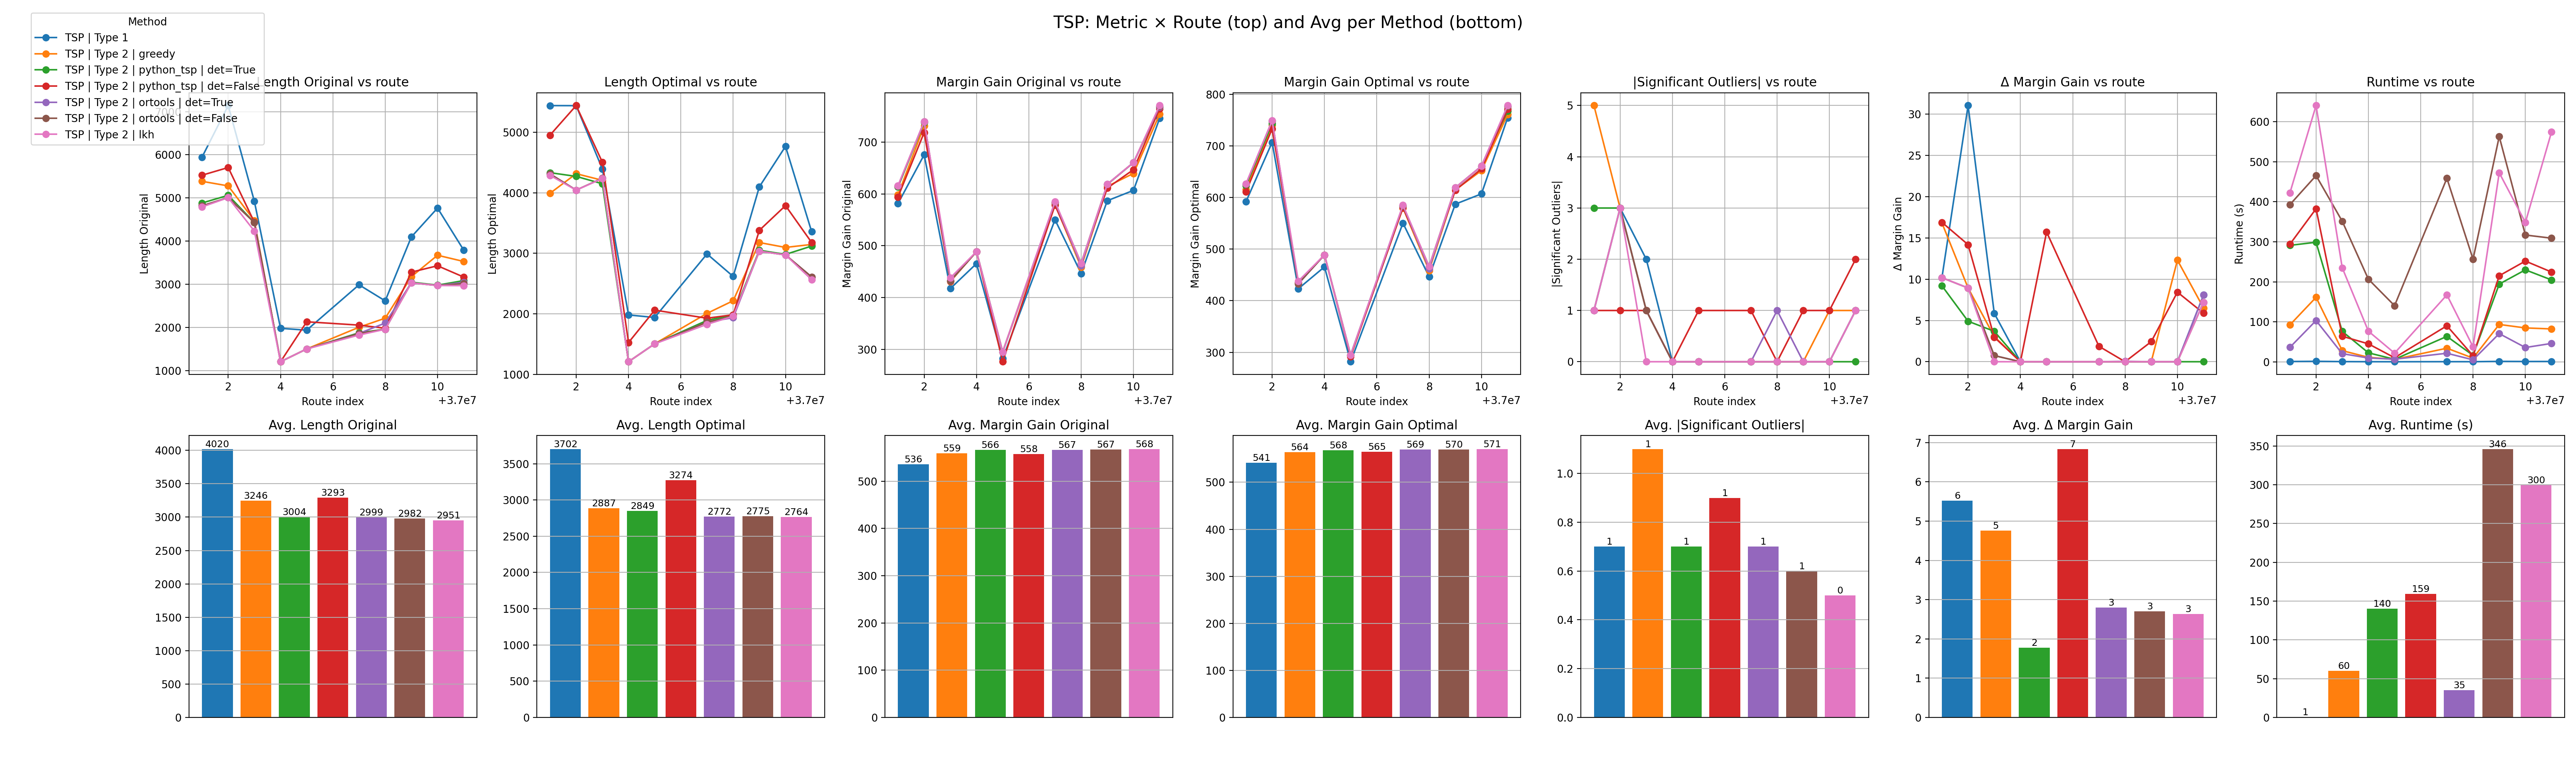
\includegraphics[width=\linewidth]{../../libraries/simulations/_img/benchmarks/hybrid/hybrid_tsp_routes.png}
\caption{Route-level hybrid benchmark panel for TSP. The top row reports route-level variation; the bottom row reports method averages for route length, optimized route length, margin gain, significant outliers, marginal gain difference, and runtime.}
\label{fig:appendix-hybrid-tsp-routes}
\end{figure}
\end{landscape}

\begin{landscape}
\begin{figure}[p]
\centering
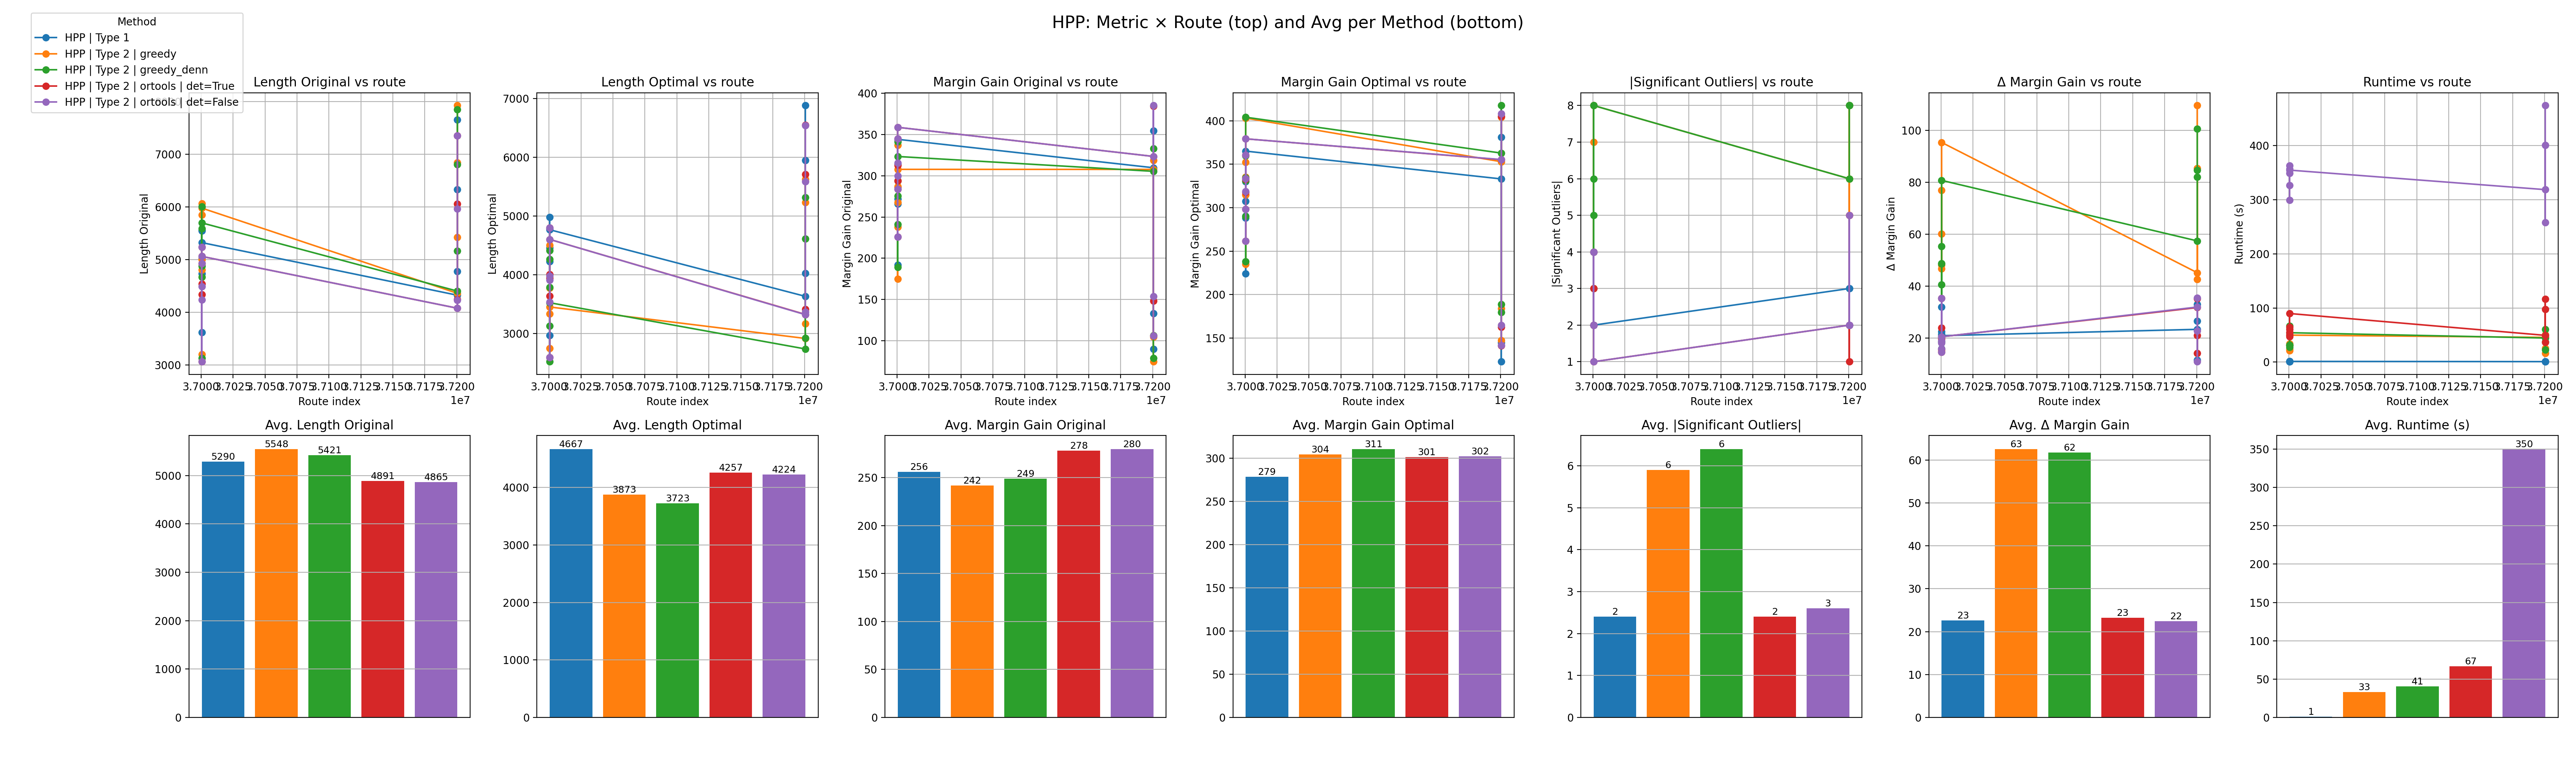
\includegraphics[width=\linewidth]{../../libraries/simulations/_img/benchmarks/hybrid/hybrid_hpp_routes.png}
\caption{Route-level hybrid benchmark panel for HPP. The top row reports route-level variation; the bottom row reports method averages for route length, optimized route length, margin gain, significant outliers, marginal gain difference, and runtime.}
\label{fig:appendix-hybrid-hpp-routes}
\end{figure}
\end{landscape}

\section{Validation Figures}
\label{app:validation-figures}

This appendix collects the large validation panels that document the approximation framework in more detail than is practical in the main text.

\subsection{Outlier Validation: TSP}

\begin{figure}[p]
\centering
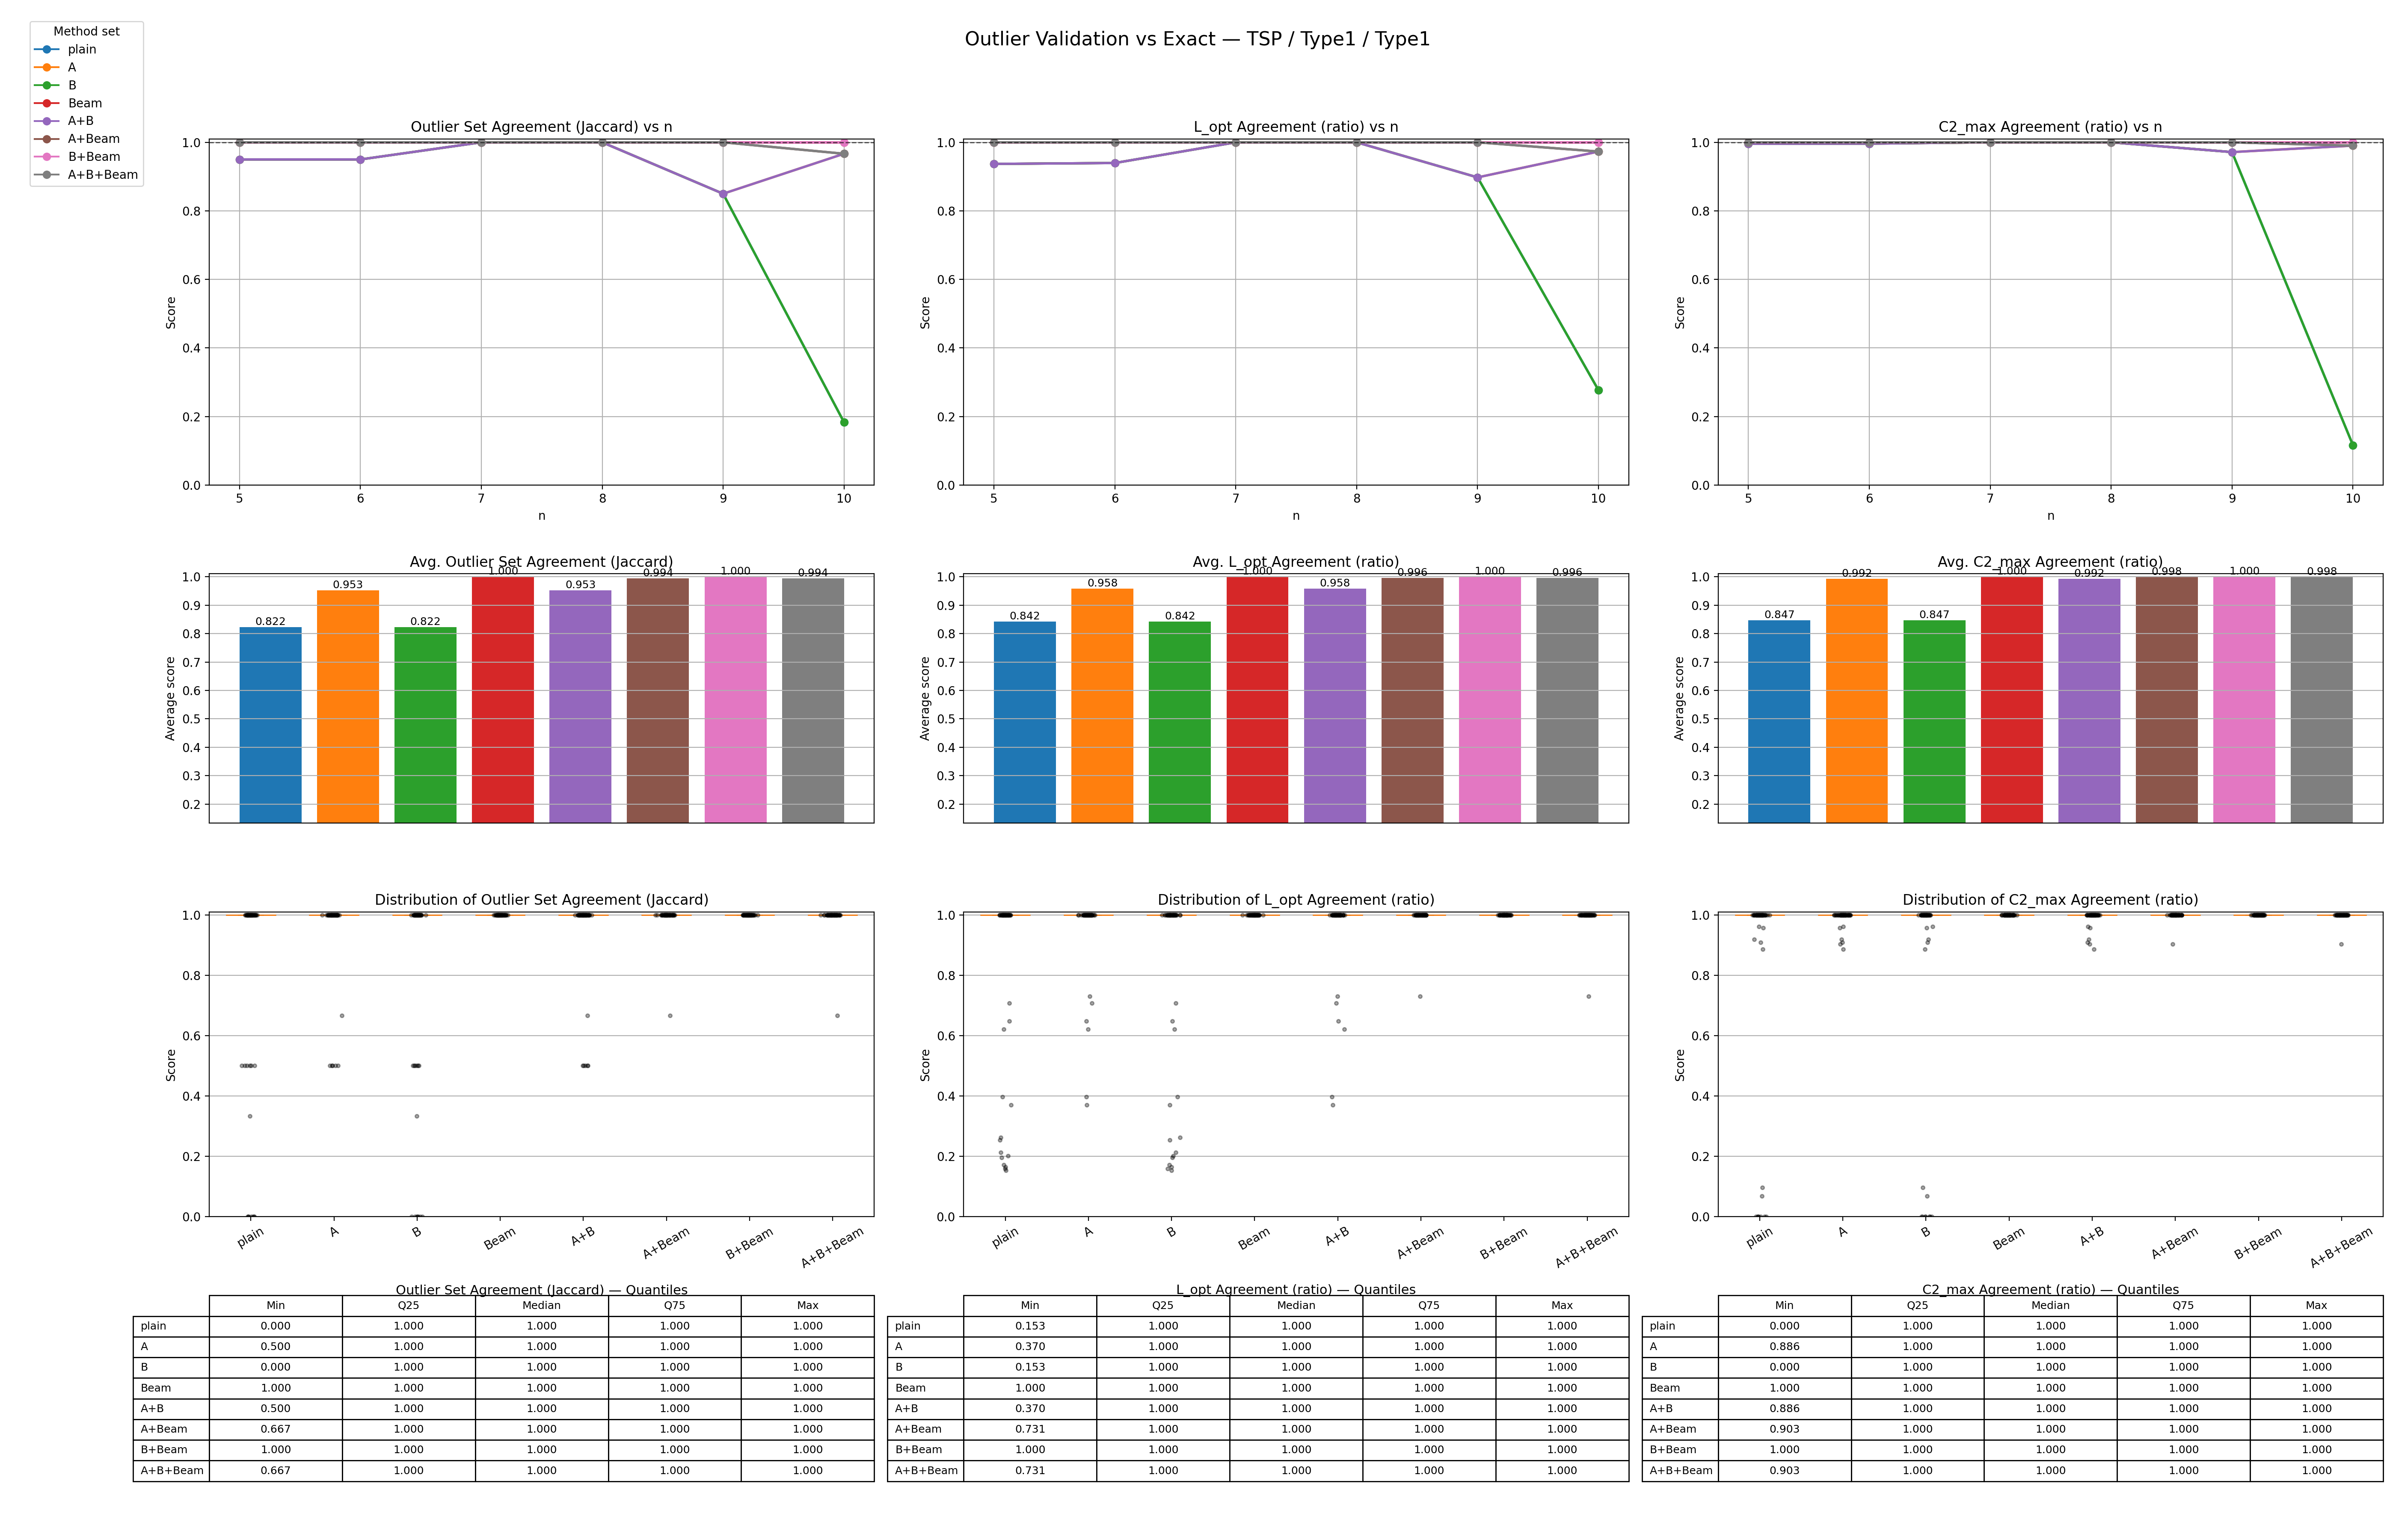
\includegraphics[width=\textwidth]{../../libraries/simulations/_img/validation/outliers/tsp/type1/Type1.png}
\caption{Detailed outlier-validation panel for TSP, Type~1.}
\label{fig:appendix-tsp-type1-validation}
\end{figure}

\begin{figure}[p]
\centering
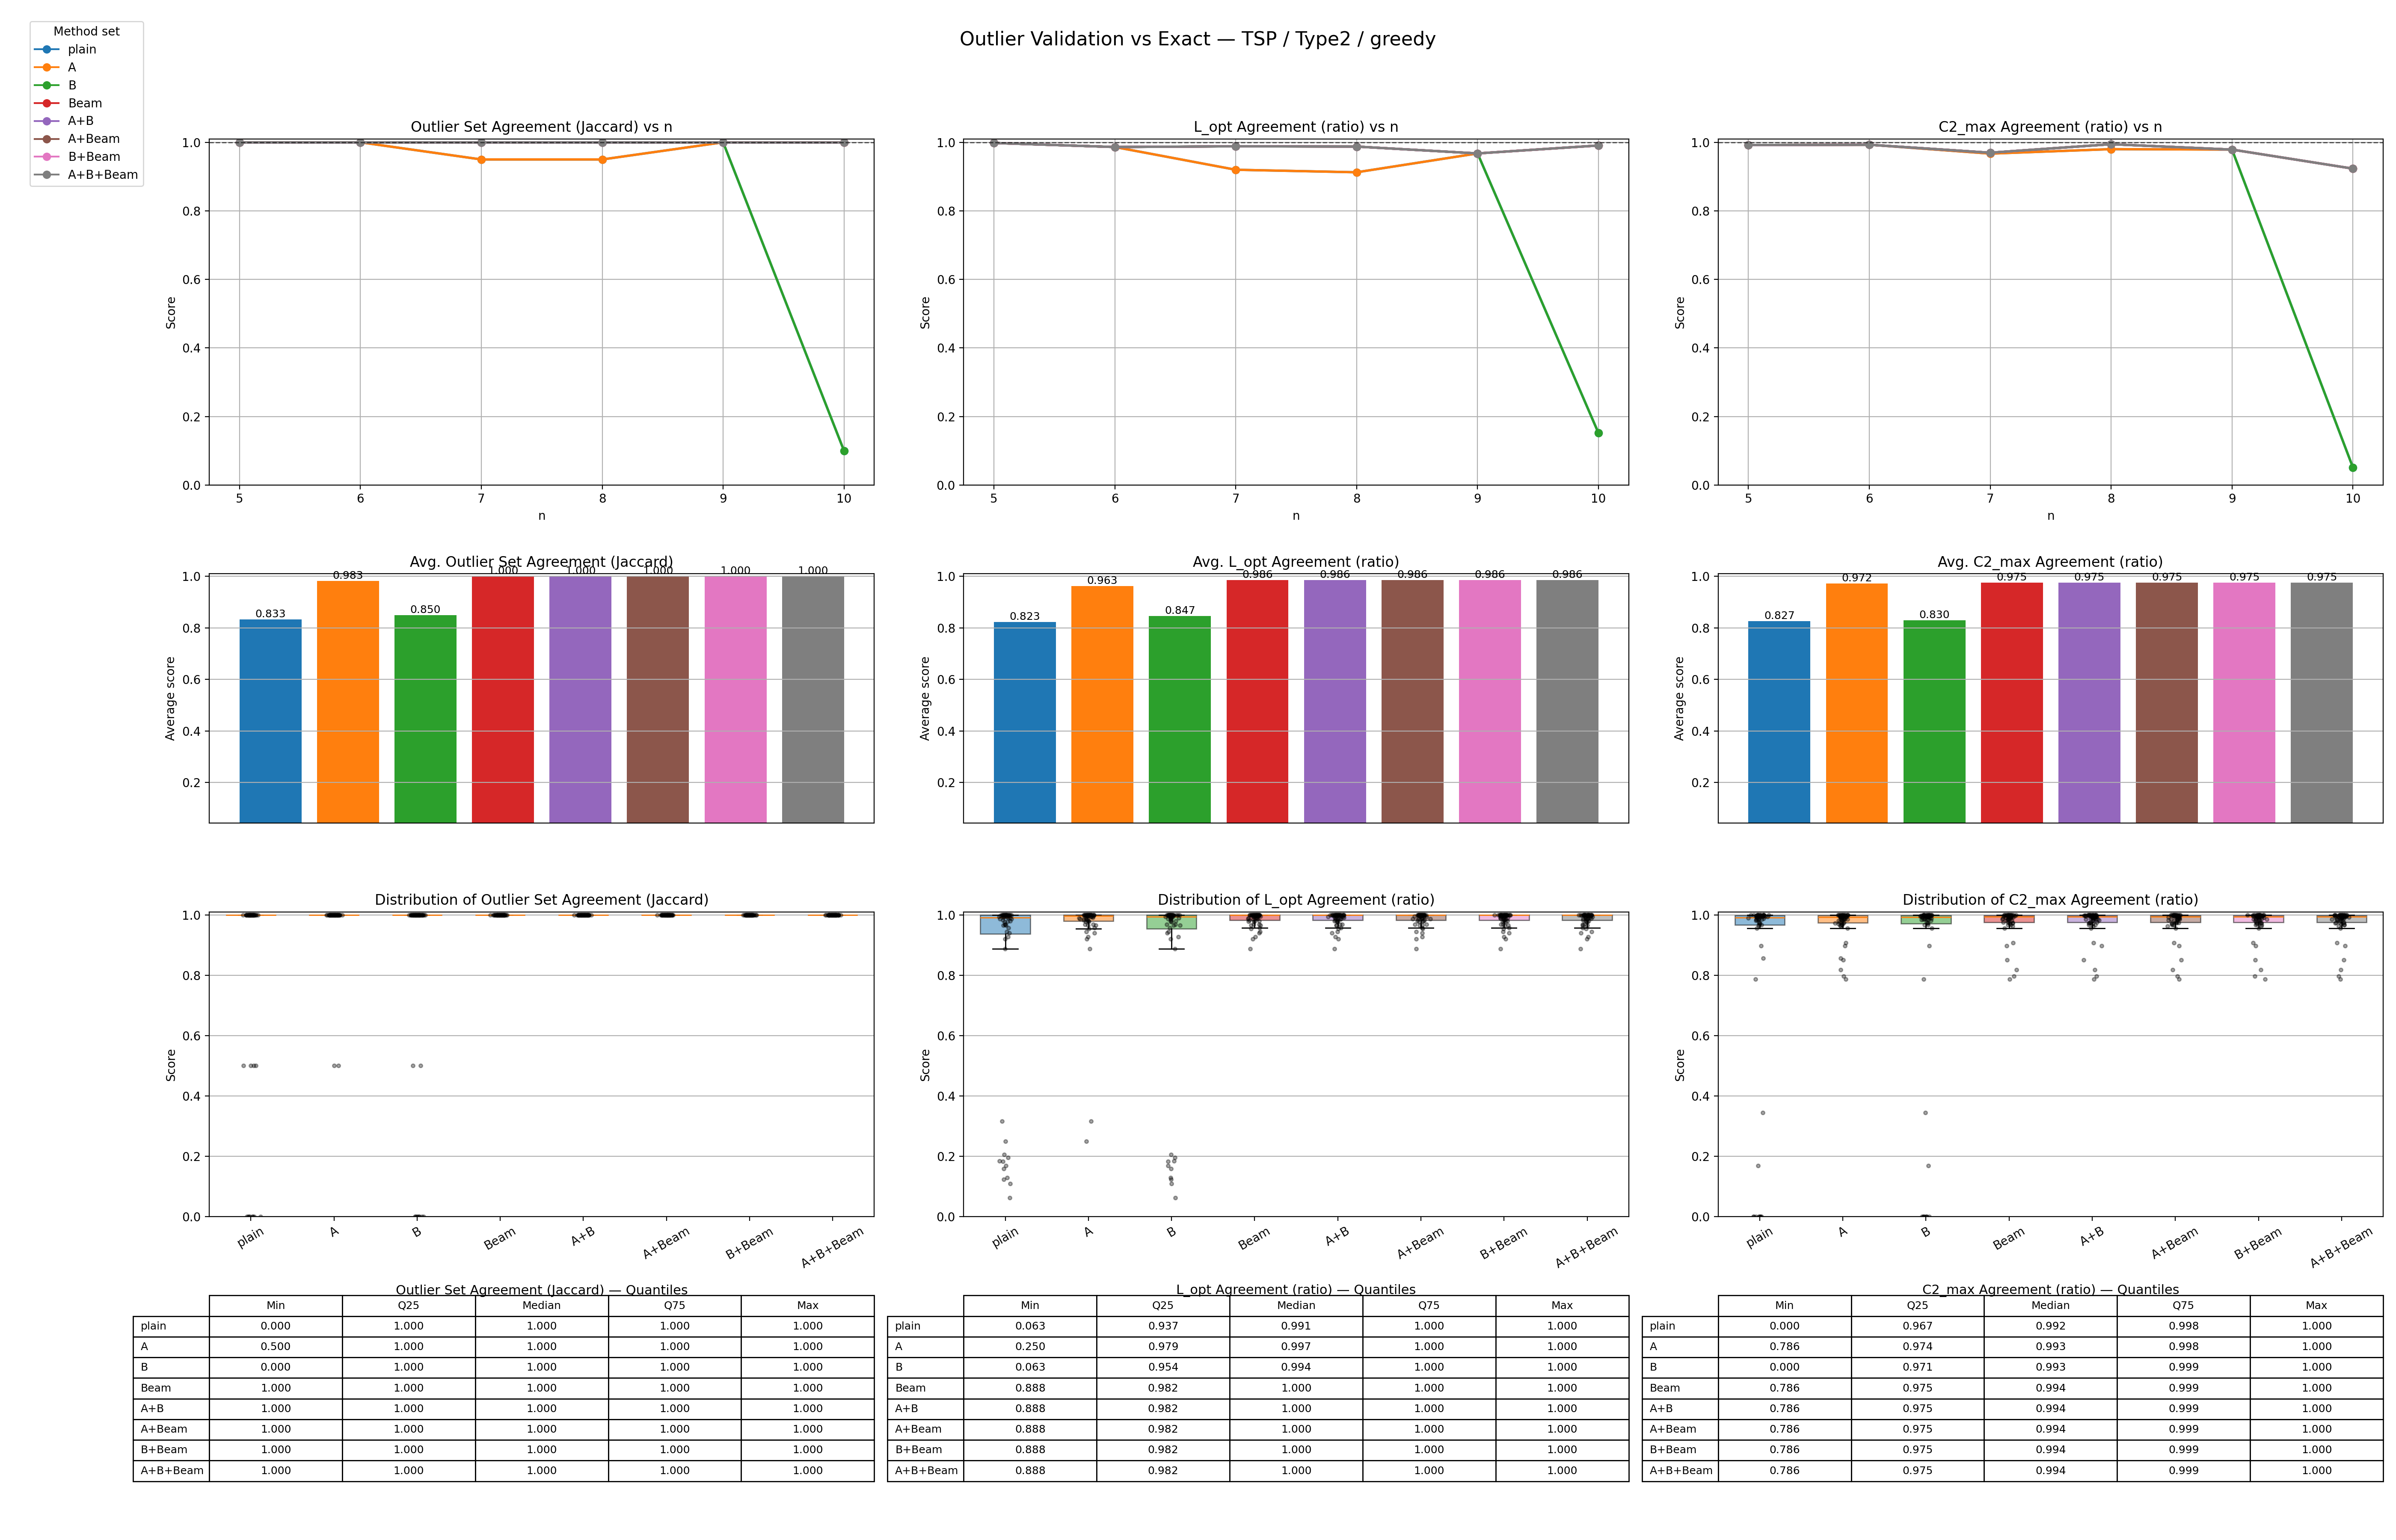
\includegraphics[width=\textwidth]{../../libraries/simulations/_img/validation/outliers/tsp/type2/greedy.png}
\caption{Detailed outlier-validation panel for TSP, Type~2, using \texttt{greedy}.}
\label{fig:appendix-tsp-type2-greedy-validation}
\end{figure}

\begin{figure}[p]
\centering
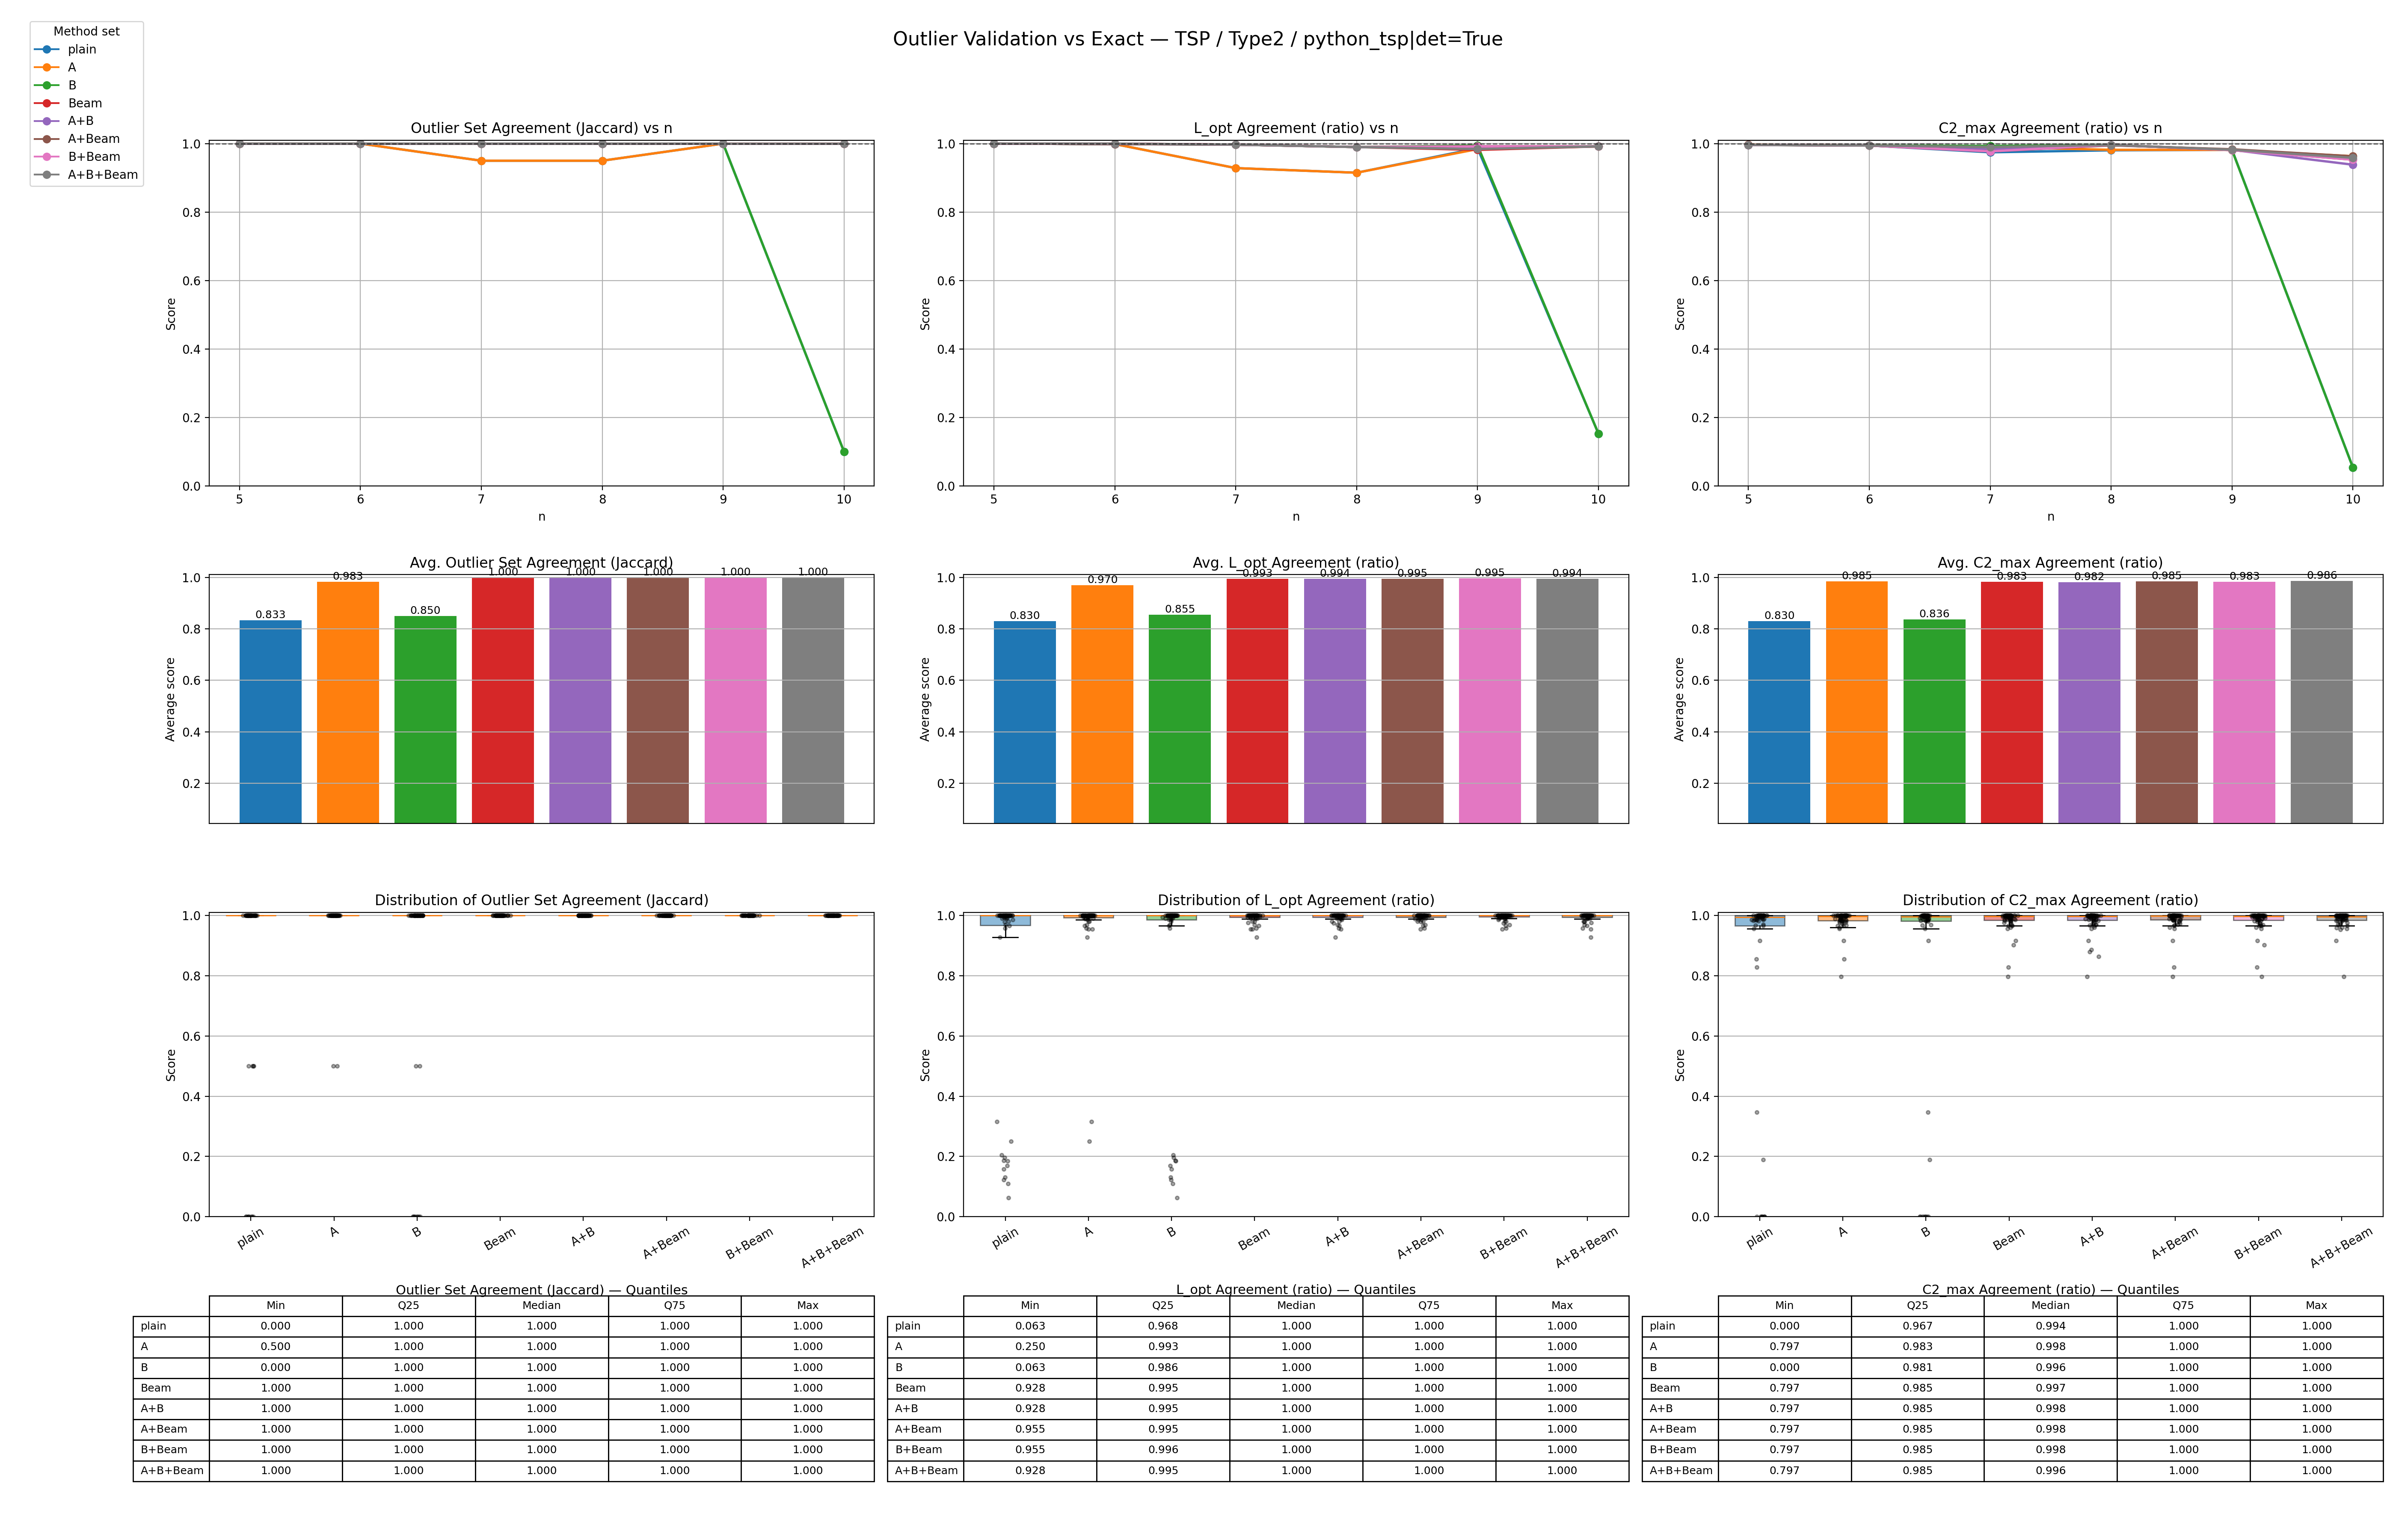
\includegraphics[width=\textwidth]{../../libraries/simulations/_img/validation/outliers/tsp/type2/python_tsp_detTrue.png}
\caption{Detailed outlier-validation panel for TSP, Type~2, using deterministic \texttt{python\_tsp}.}
\label{fig:appendix-tsp-type2-python-det-true-validation}
\end{figure}

\begin{figure}[p]
\centering
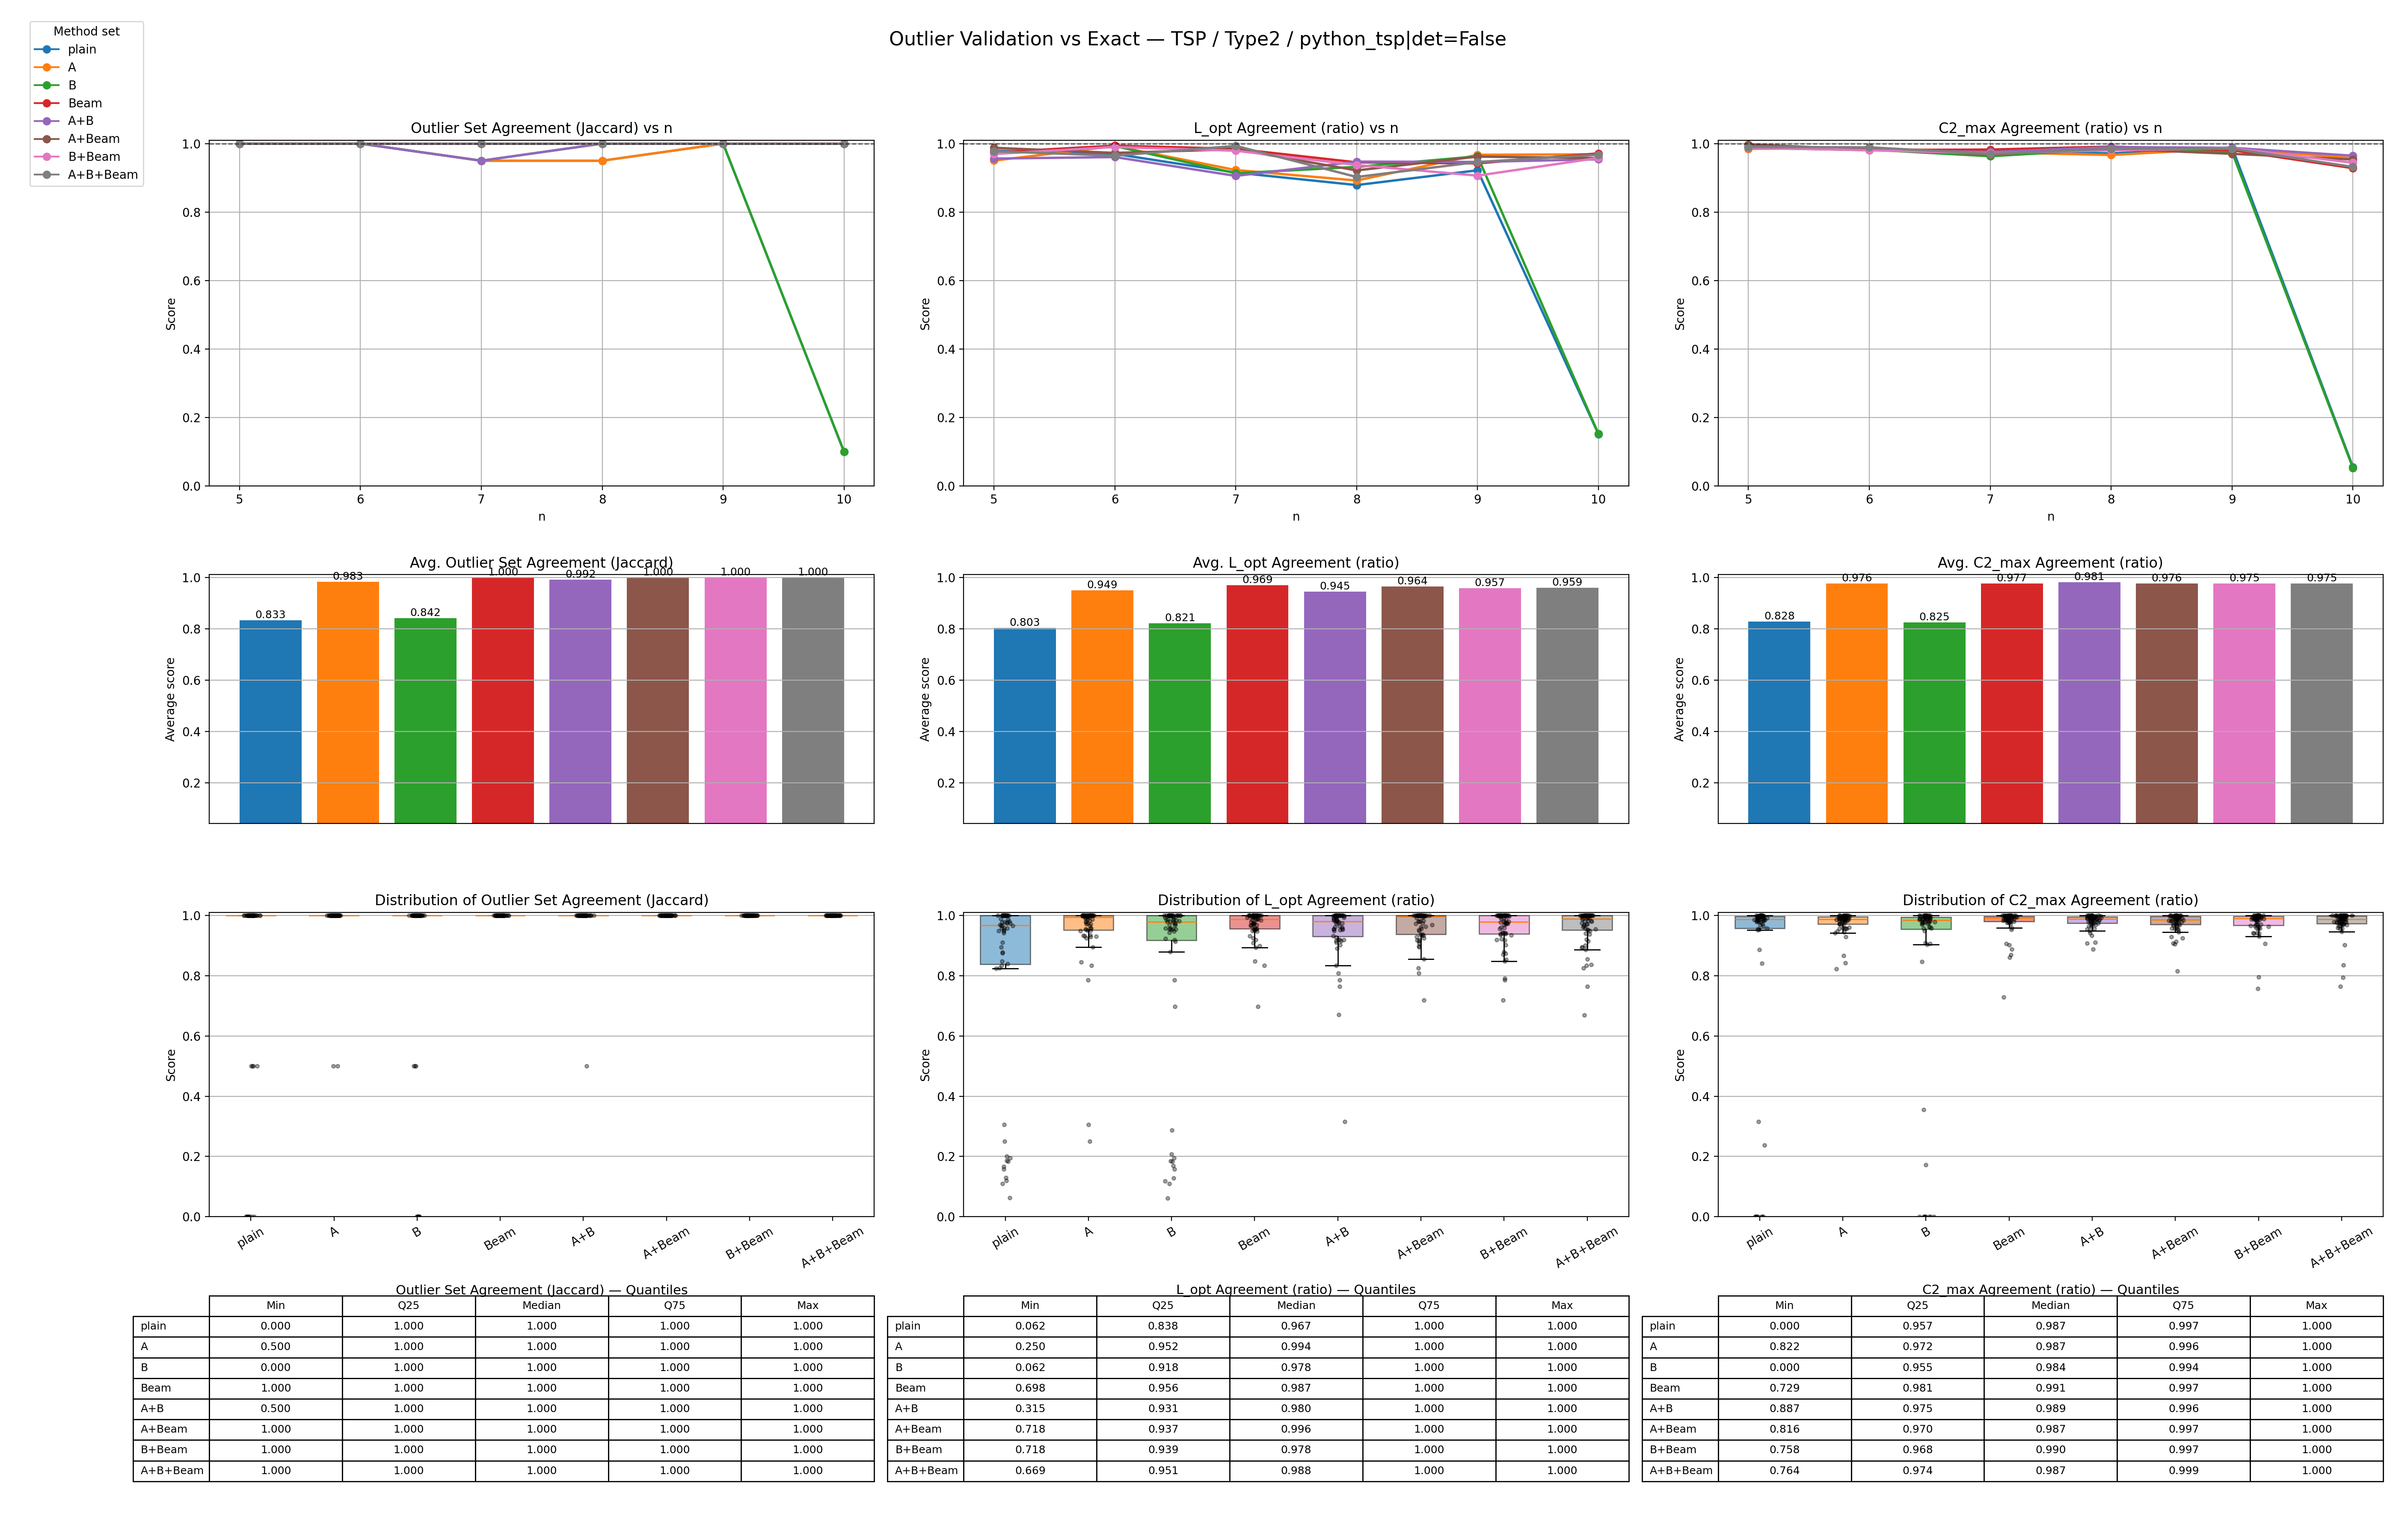
\includegraphics[width=\textwidth]{../../libraries/simulations/_img/validation/outliers/tsp/type2/python_tsp_detFalse.png}
\caption{Detailed outlier-validation panel for TSP, Type~2, using non-deterministic \texttt{python\_tsp}.}
\label{fig:appendix-tsp-type2-python-det-false-validation}
\end{figure}

\begin{figure}[p]
\centering
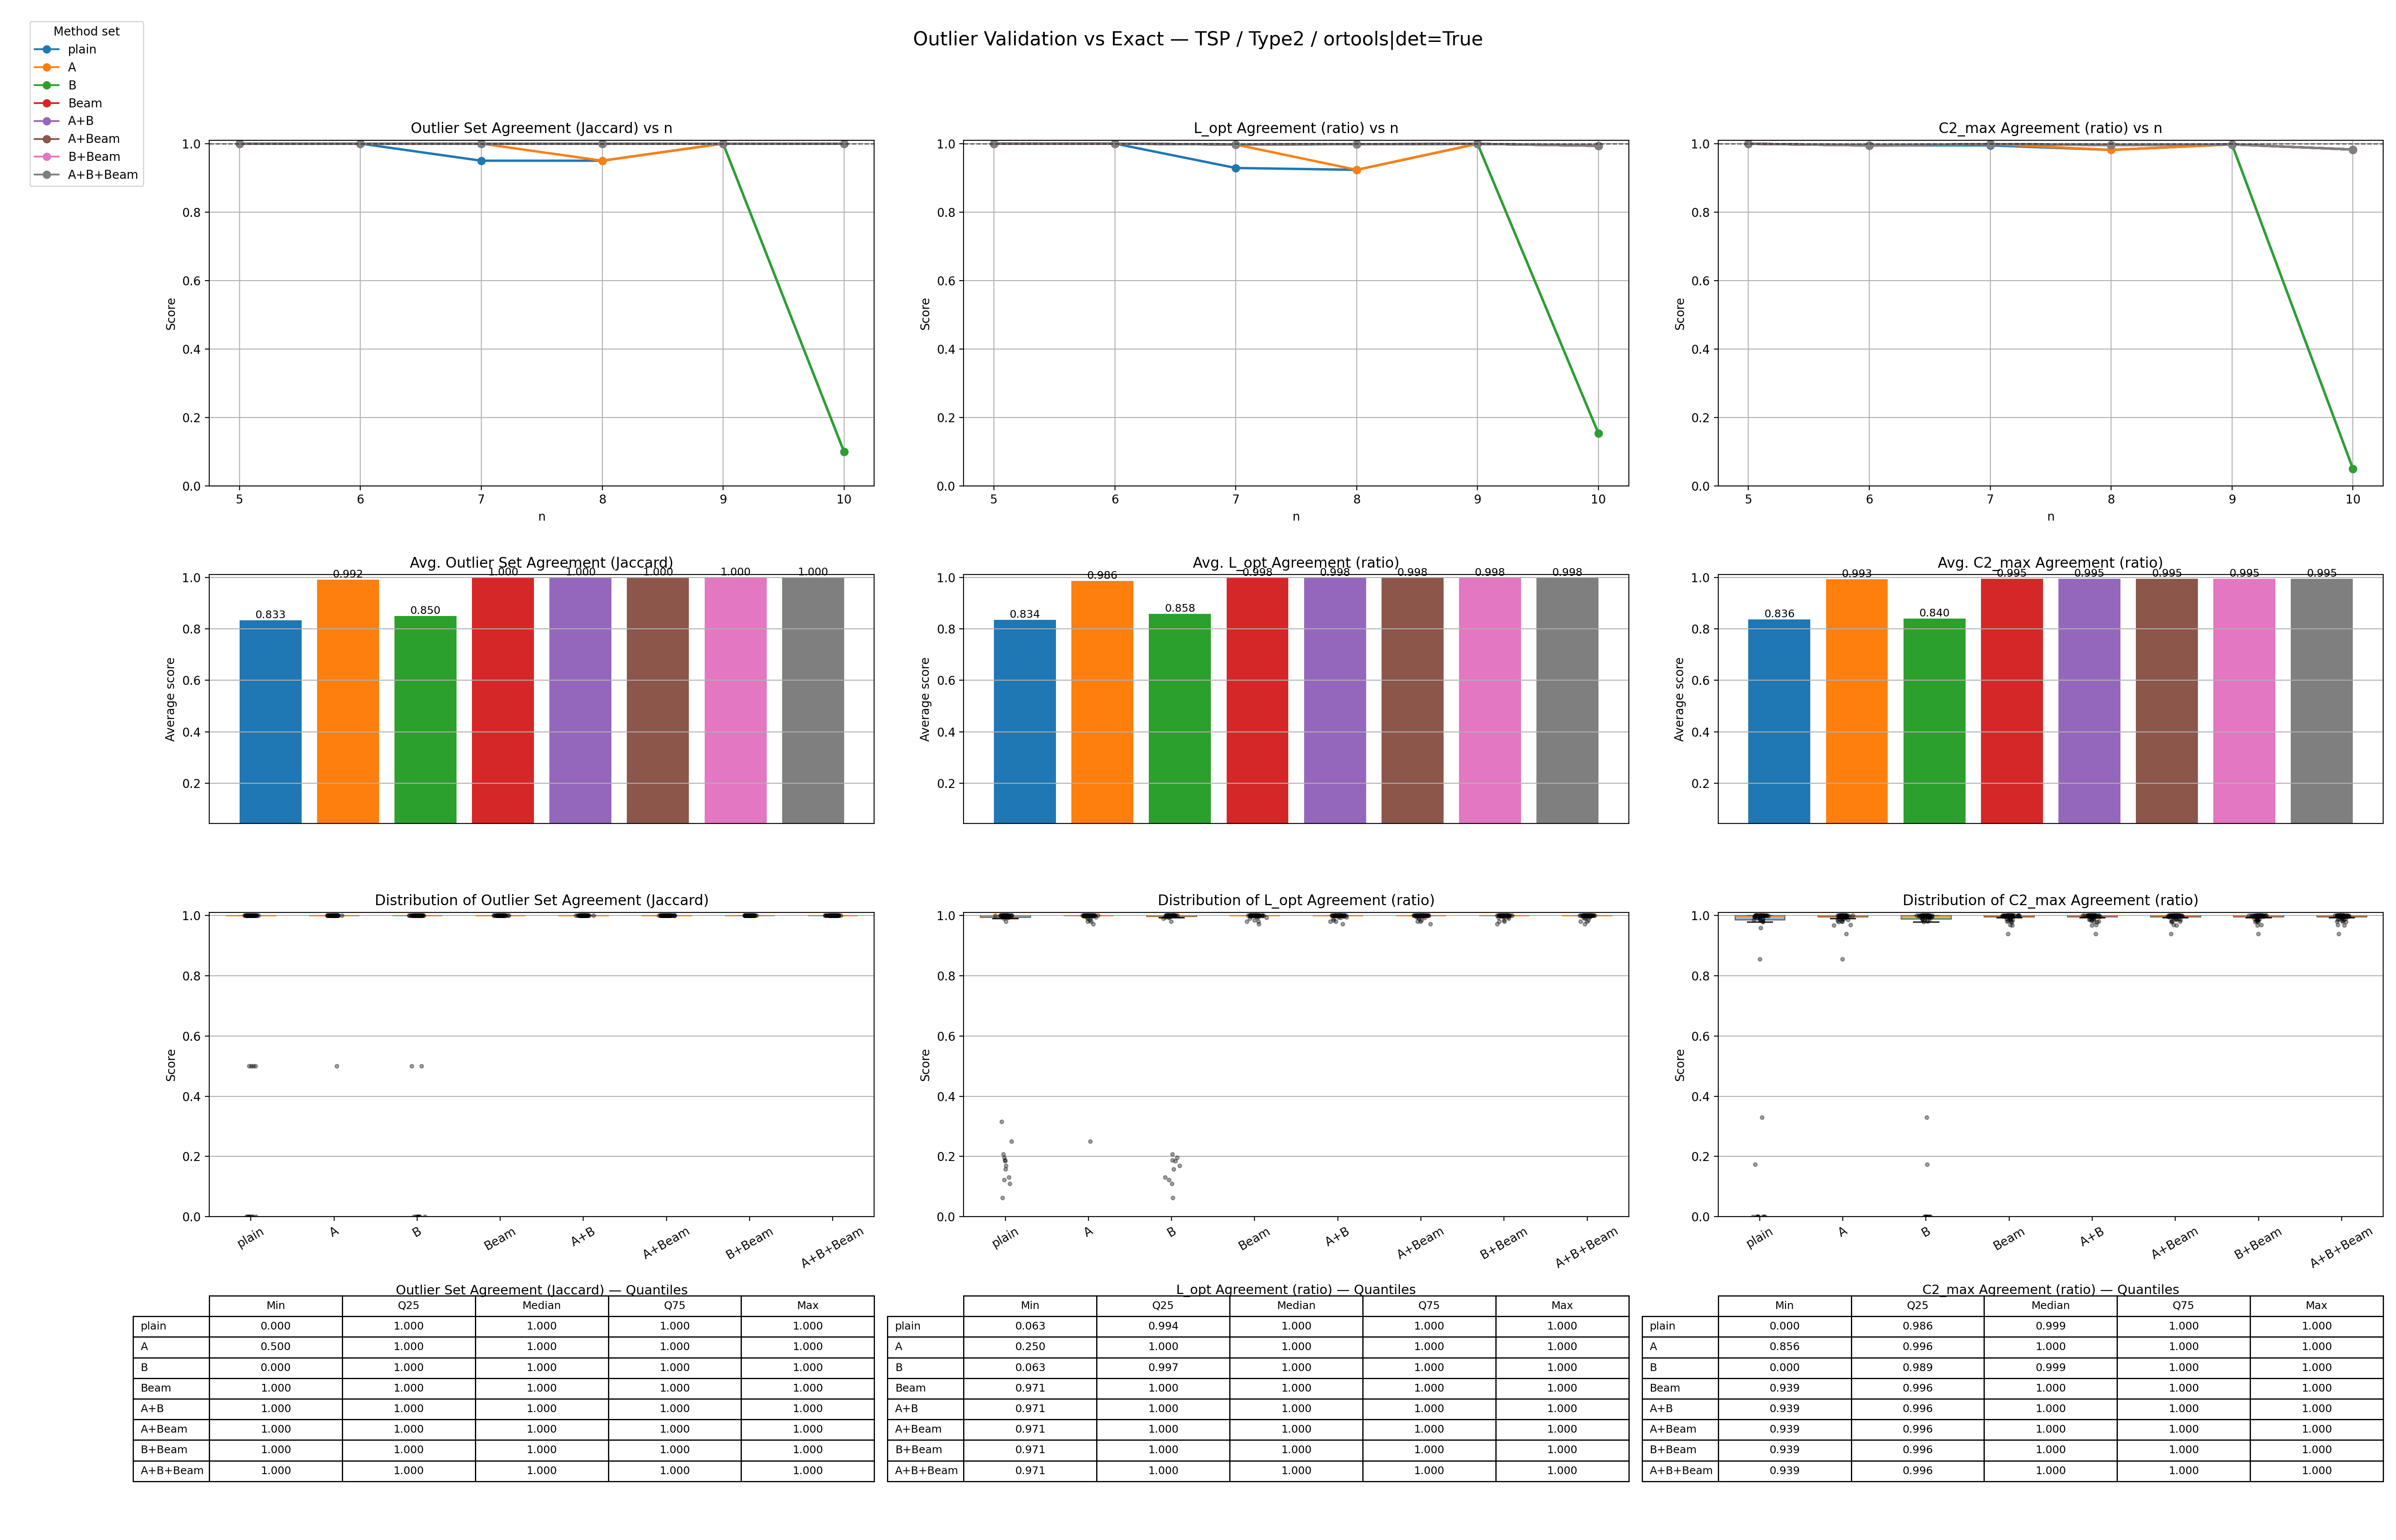
\includegraphics[width=\textwidth]{../../libraries/simulations/_img/validation/outliers/tsp/type2/ortools_detTrue.png}
\caption{Detailed outlier-validation panel for TSP, Type~2, using deterministic \texttt{ortools}.}
\label{fig:appendix-tsp-type2-validation}
\end{figure}

\begin{figure}[p]
\centering
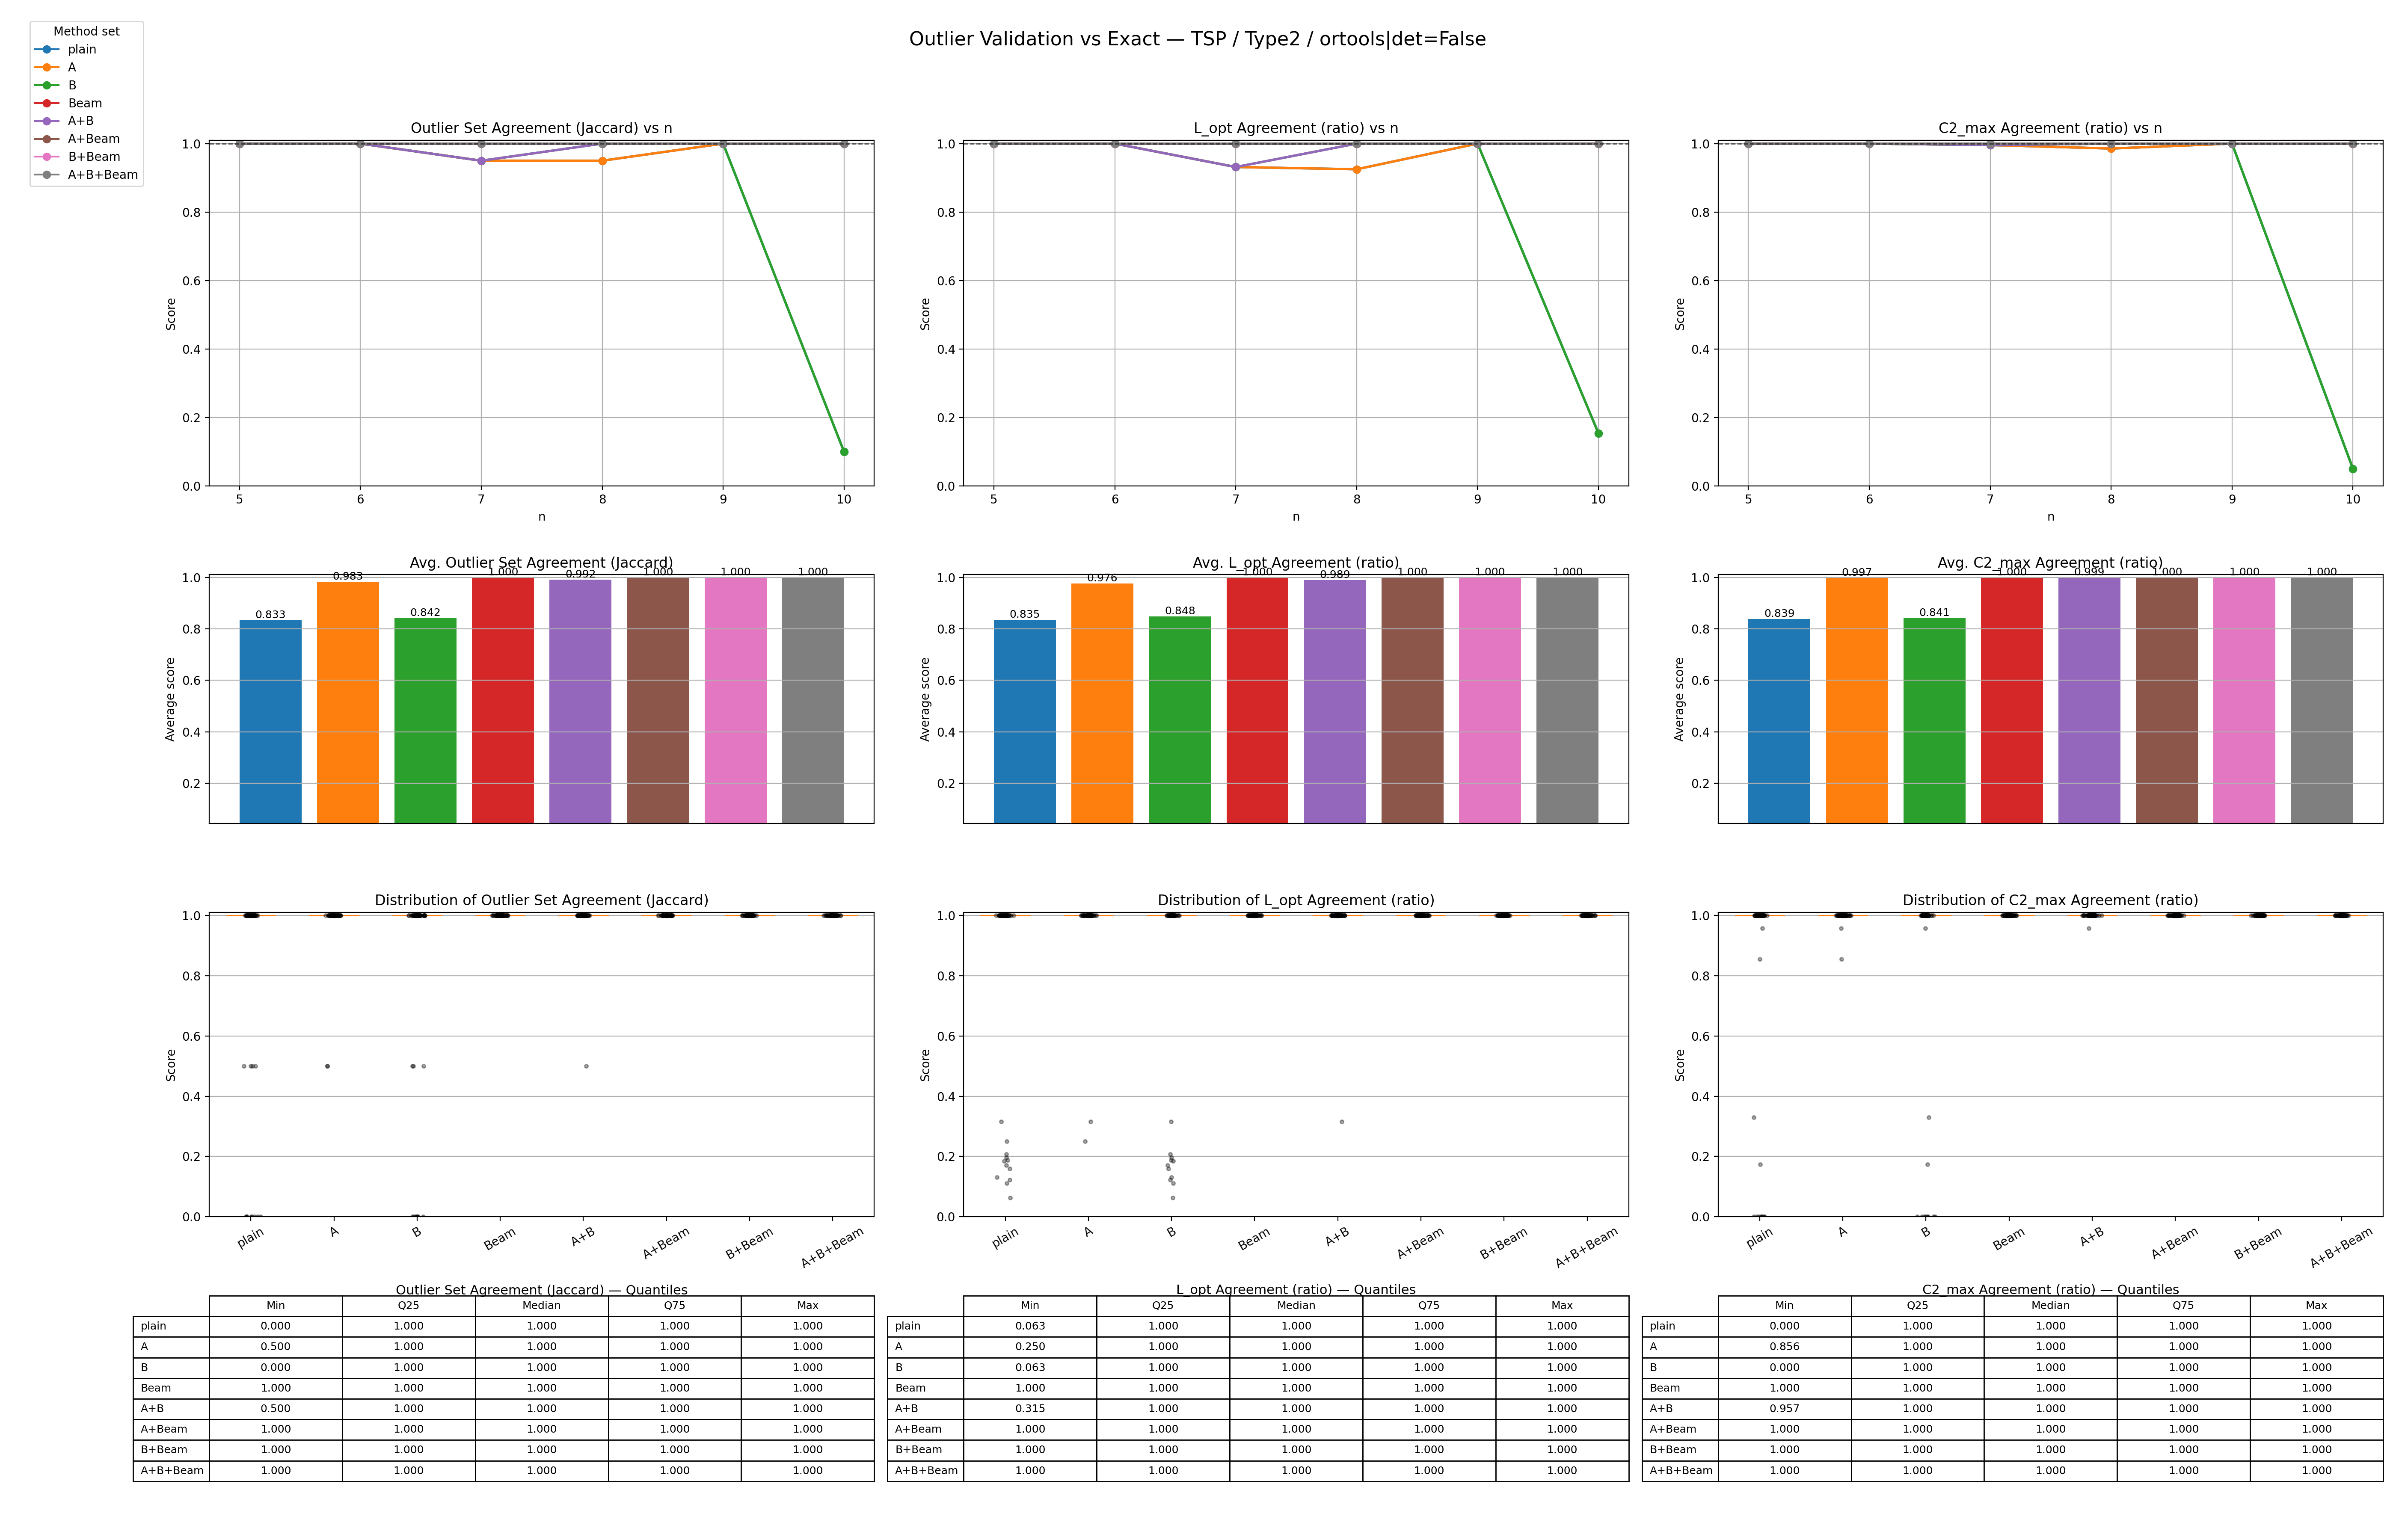
\includegraphics[width=\textwidth]{../../libraries/simulations/_img/validation/outliers/tsp/type2/ortools_detFalse.png}
\caption{Detailed outlier-validation panel for TSP, Type~2, using non-deterministic \texttt{ortools}.}
\label{fig:appendix-tsp-type2-ortools-det-false-validation}
\end{figure}

\begin{figure}[p]
\centering
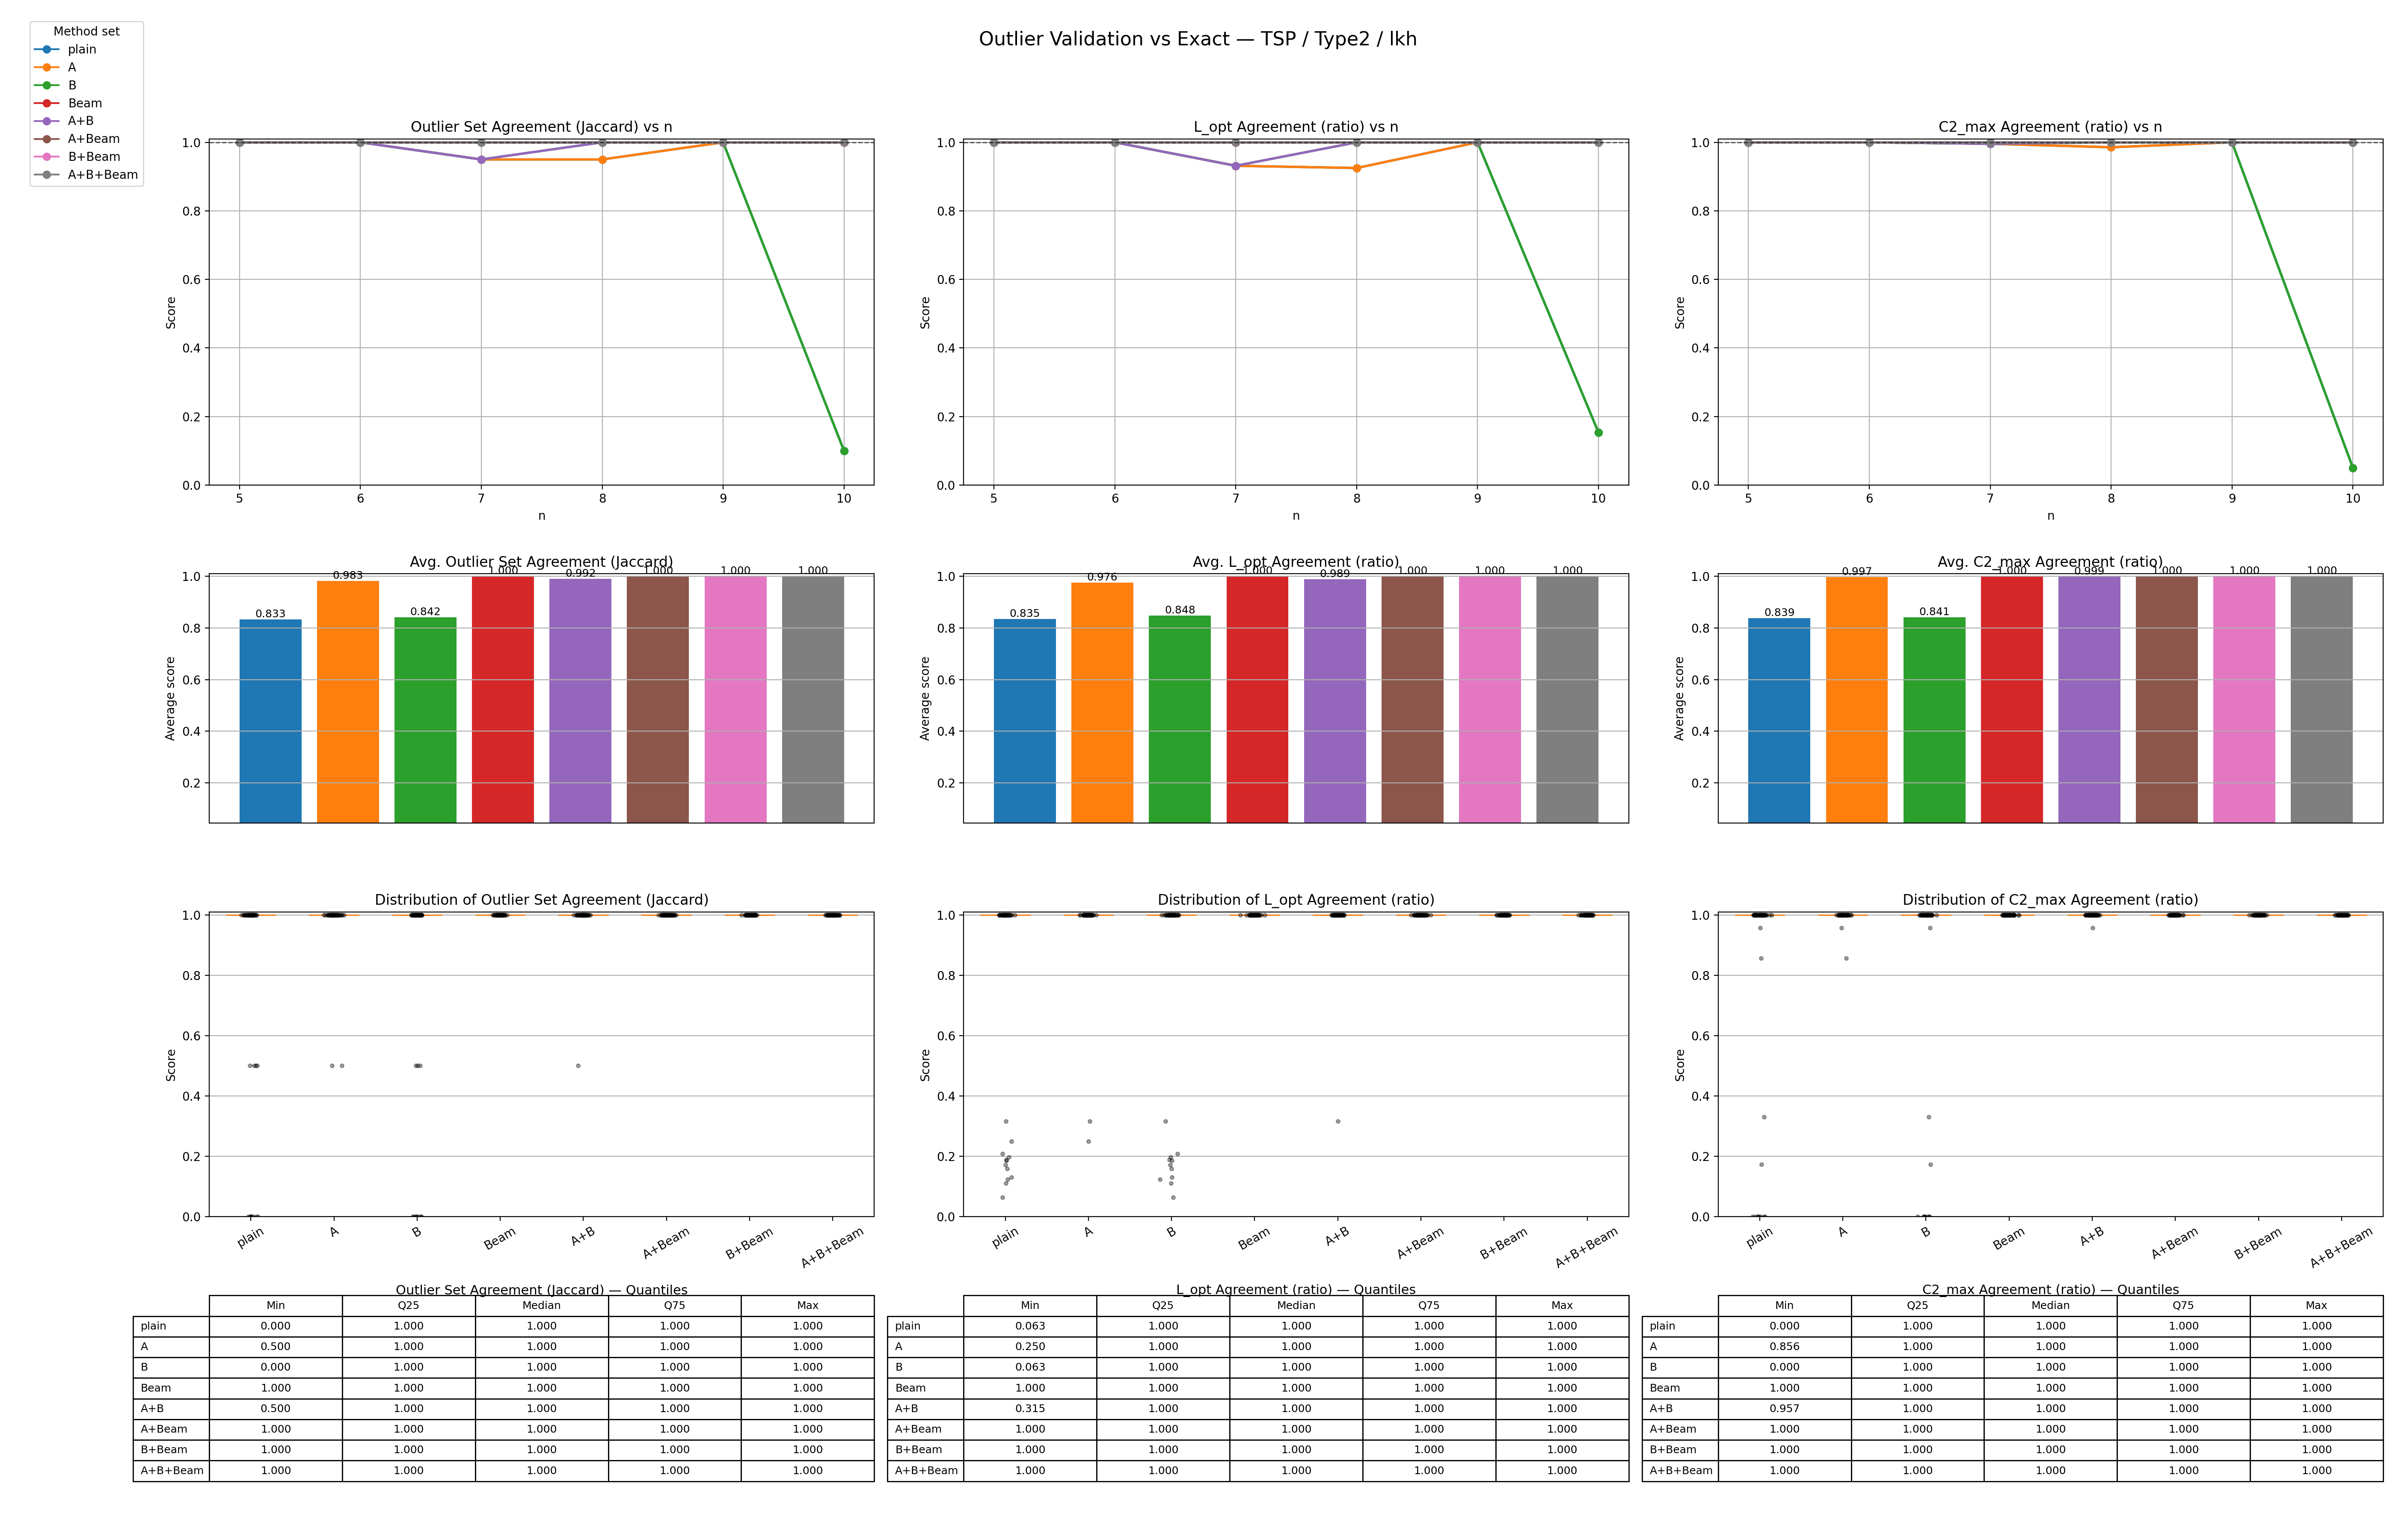
\includegraphics[width=\textwidth]{../../libraries/simulations/_img/validation/outliers/tsp/type2/lkh.png}
\caption{Detailed outlier-validation panel for TSP, Type~2, using \texttt{lkh}.}
\label{fig:appendix-tsp-type2-lkh-validation}
\end{figure}

\subsection{Outlier Validation: HPP}

\begin{figure}[p]
\centering
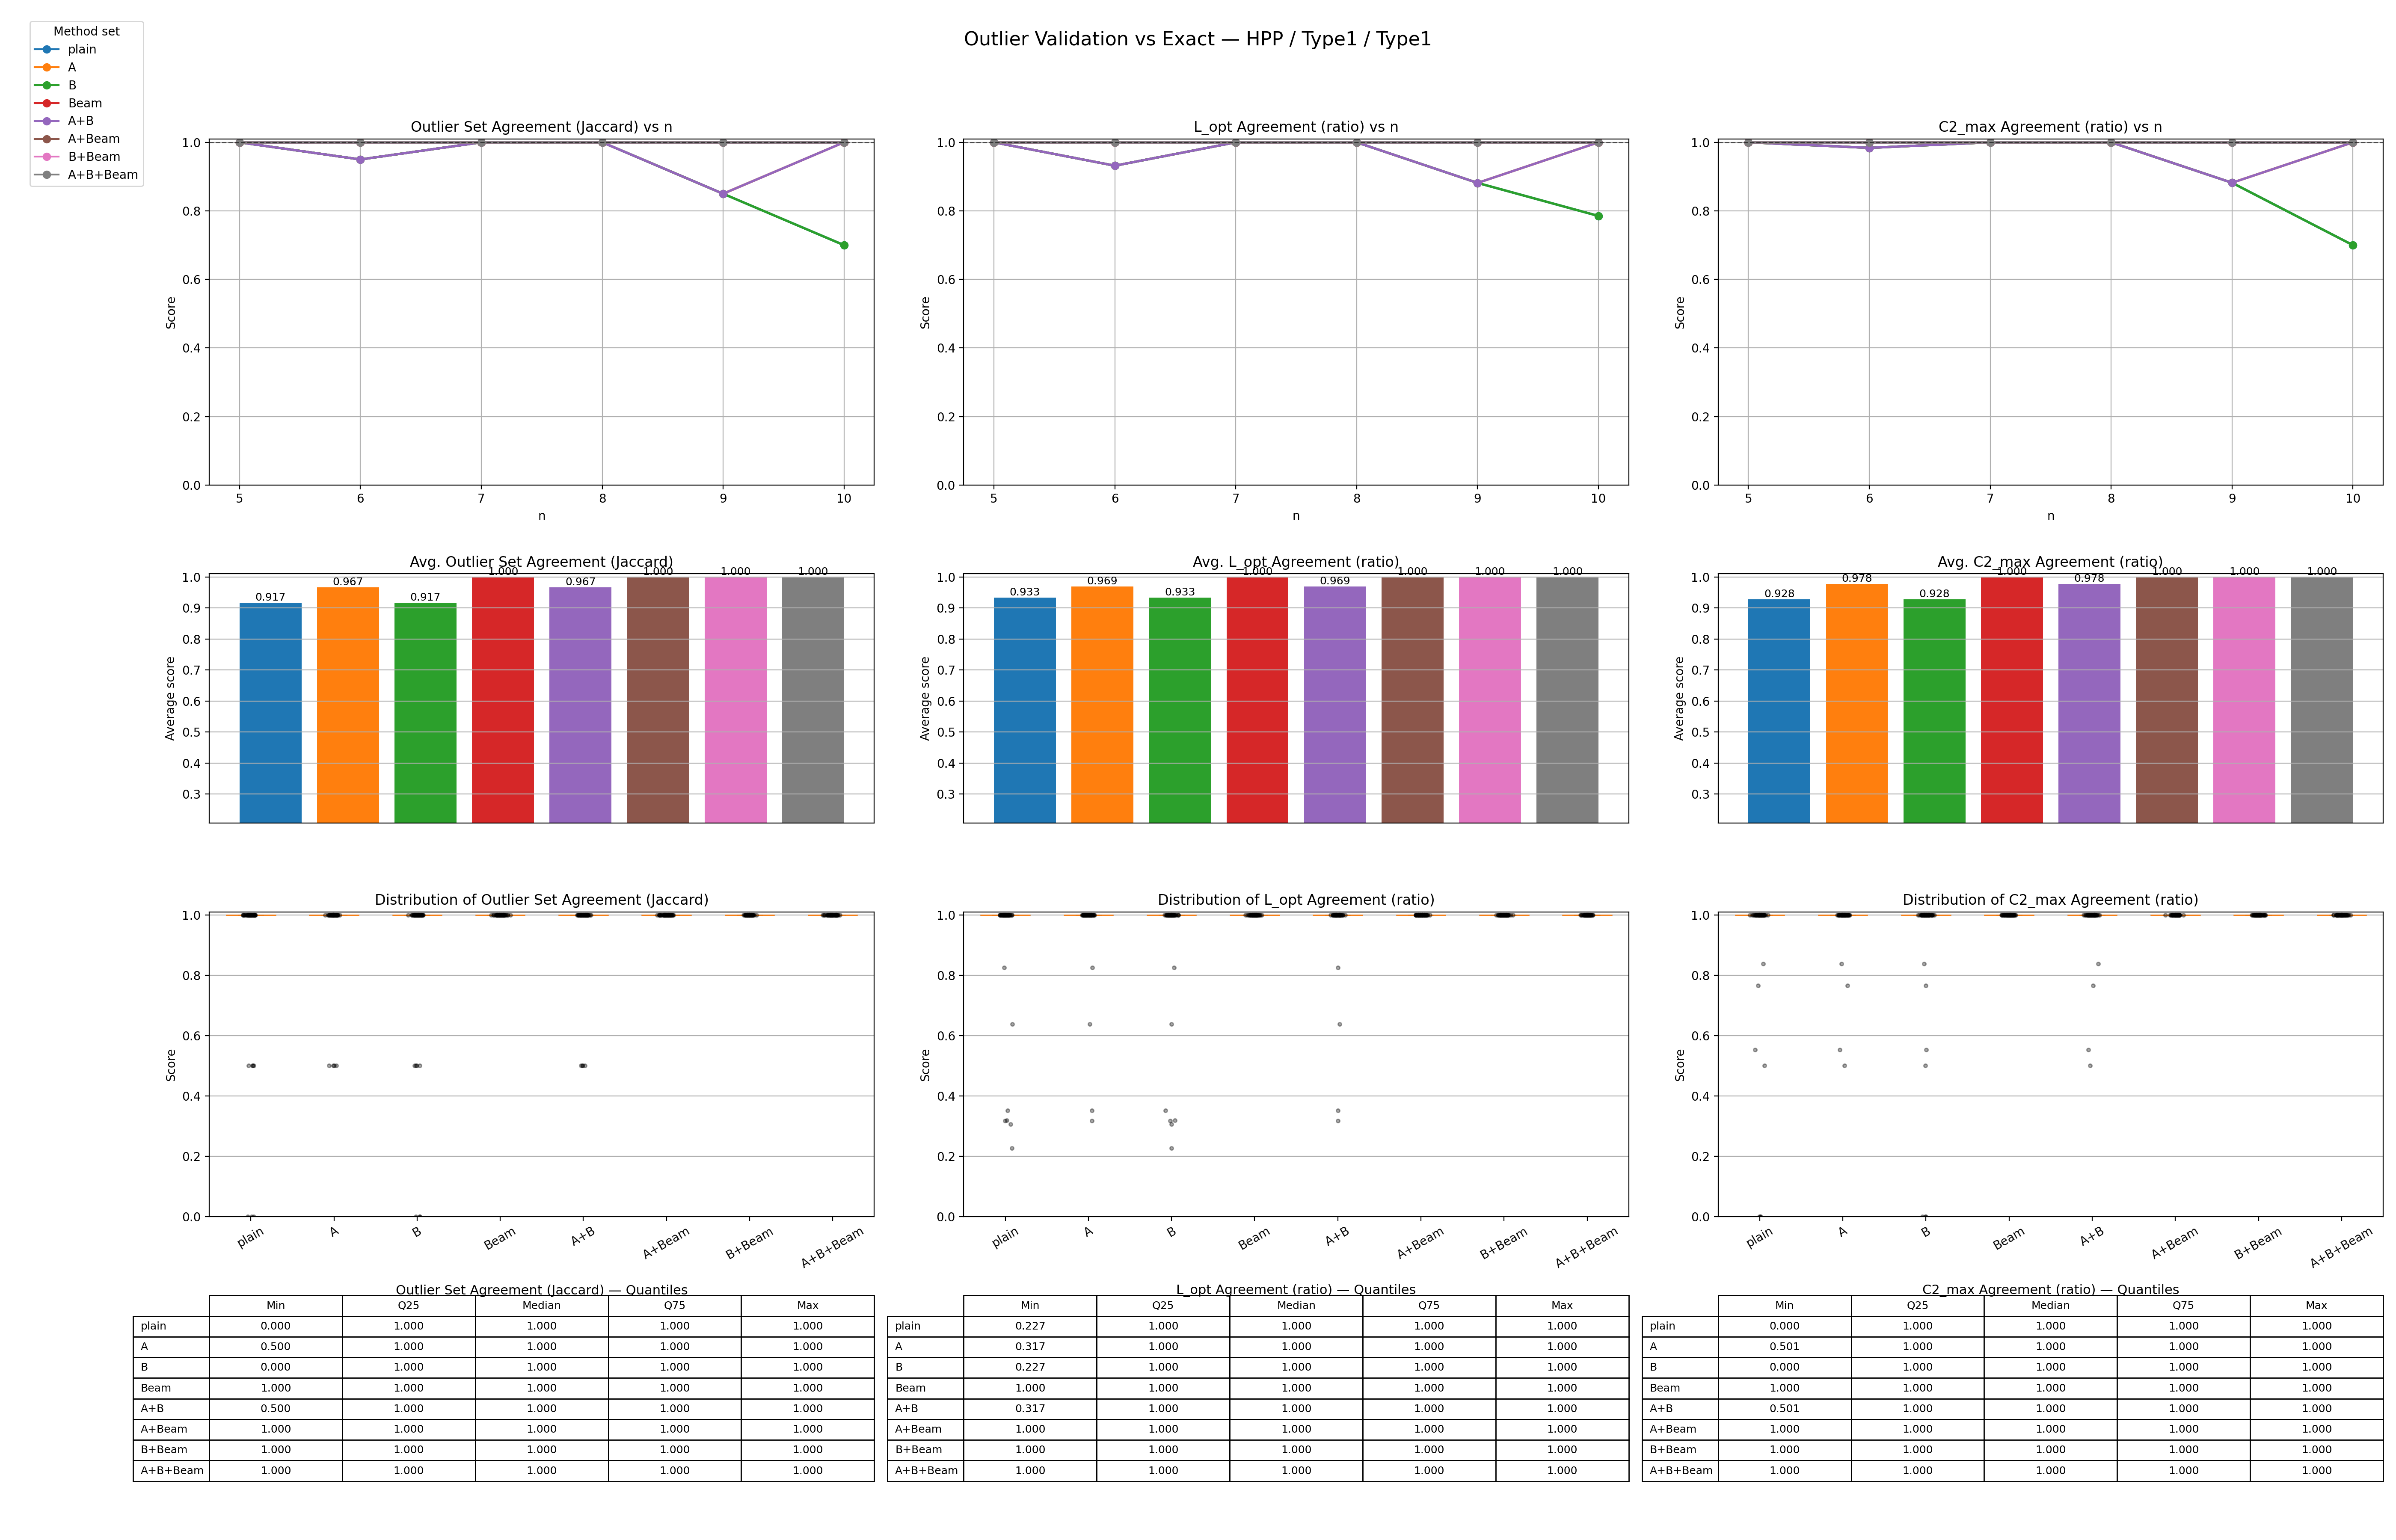
\includegraphics[width=\textwidth]{../../libraries/simulations/_img/validation/outliers/hpp/type1/Type1.png}
\caption{Detailed outlier-validation panel for HPP, Type~1.}
\label{fig:appendix-hpp-type1-validation}
\end{figure}

\begin{figure}[p]
\centering
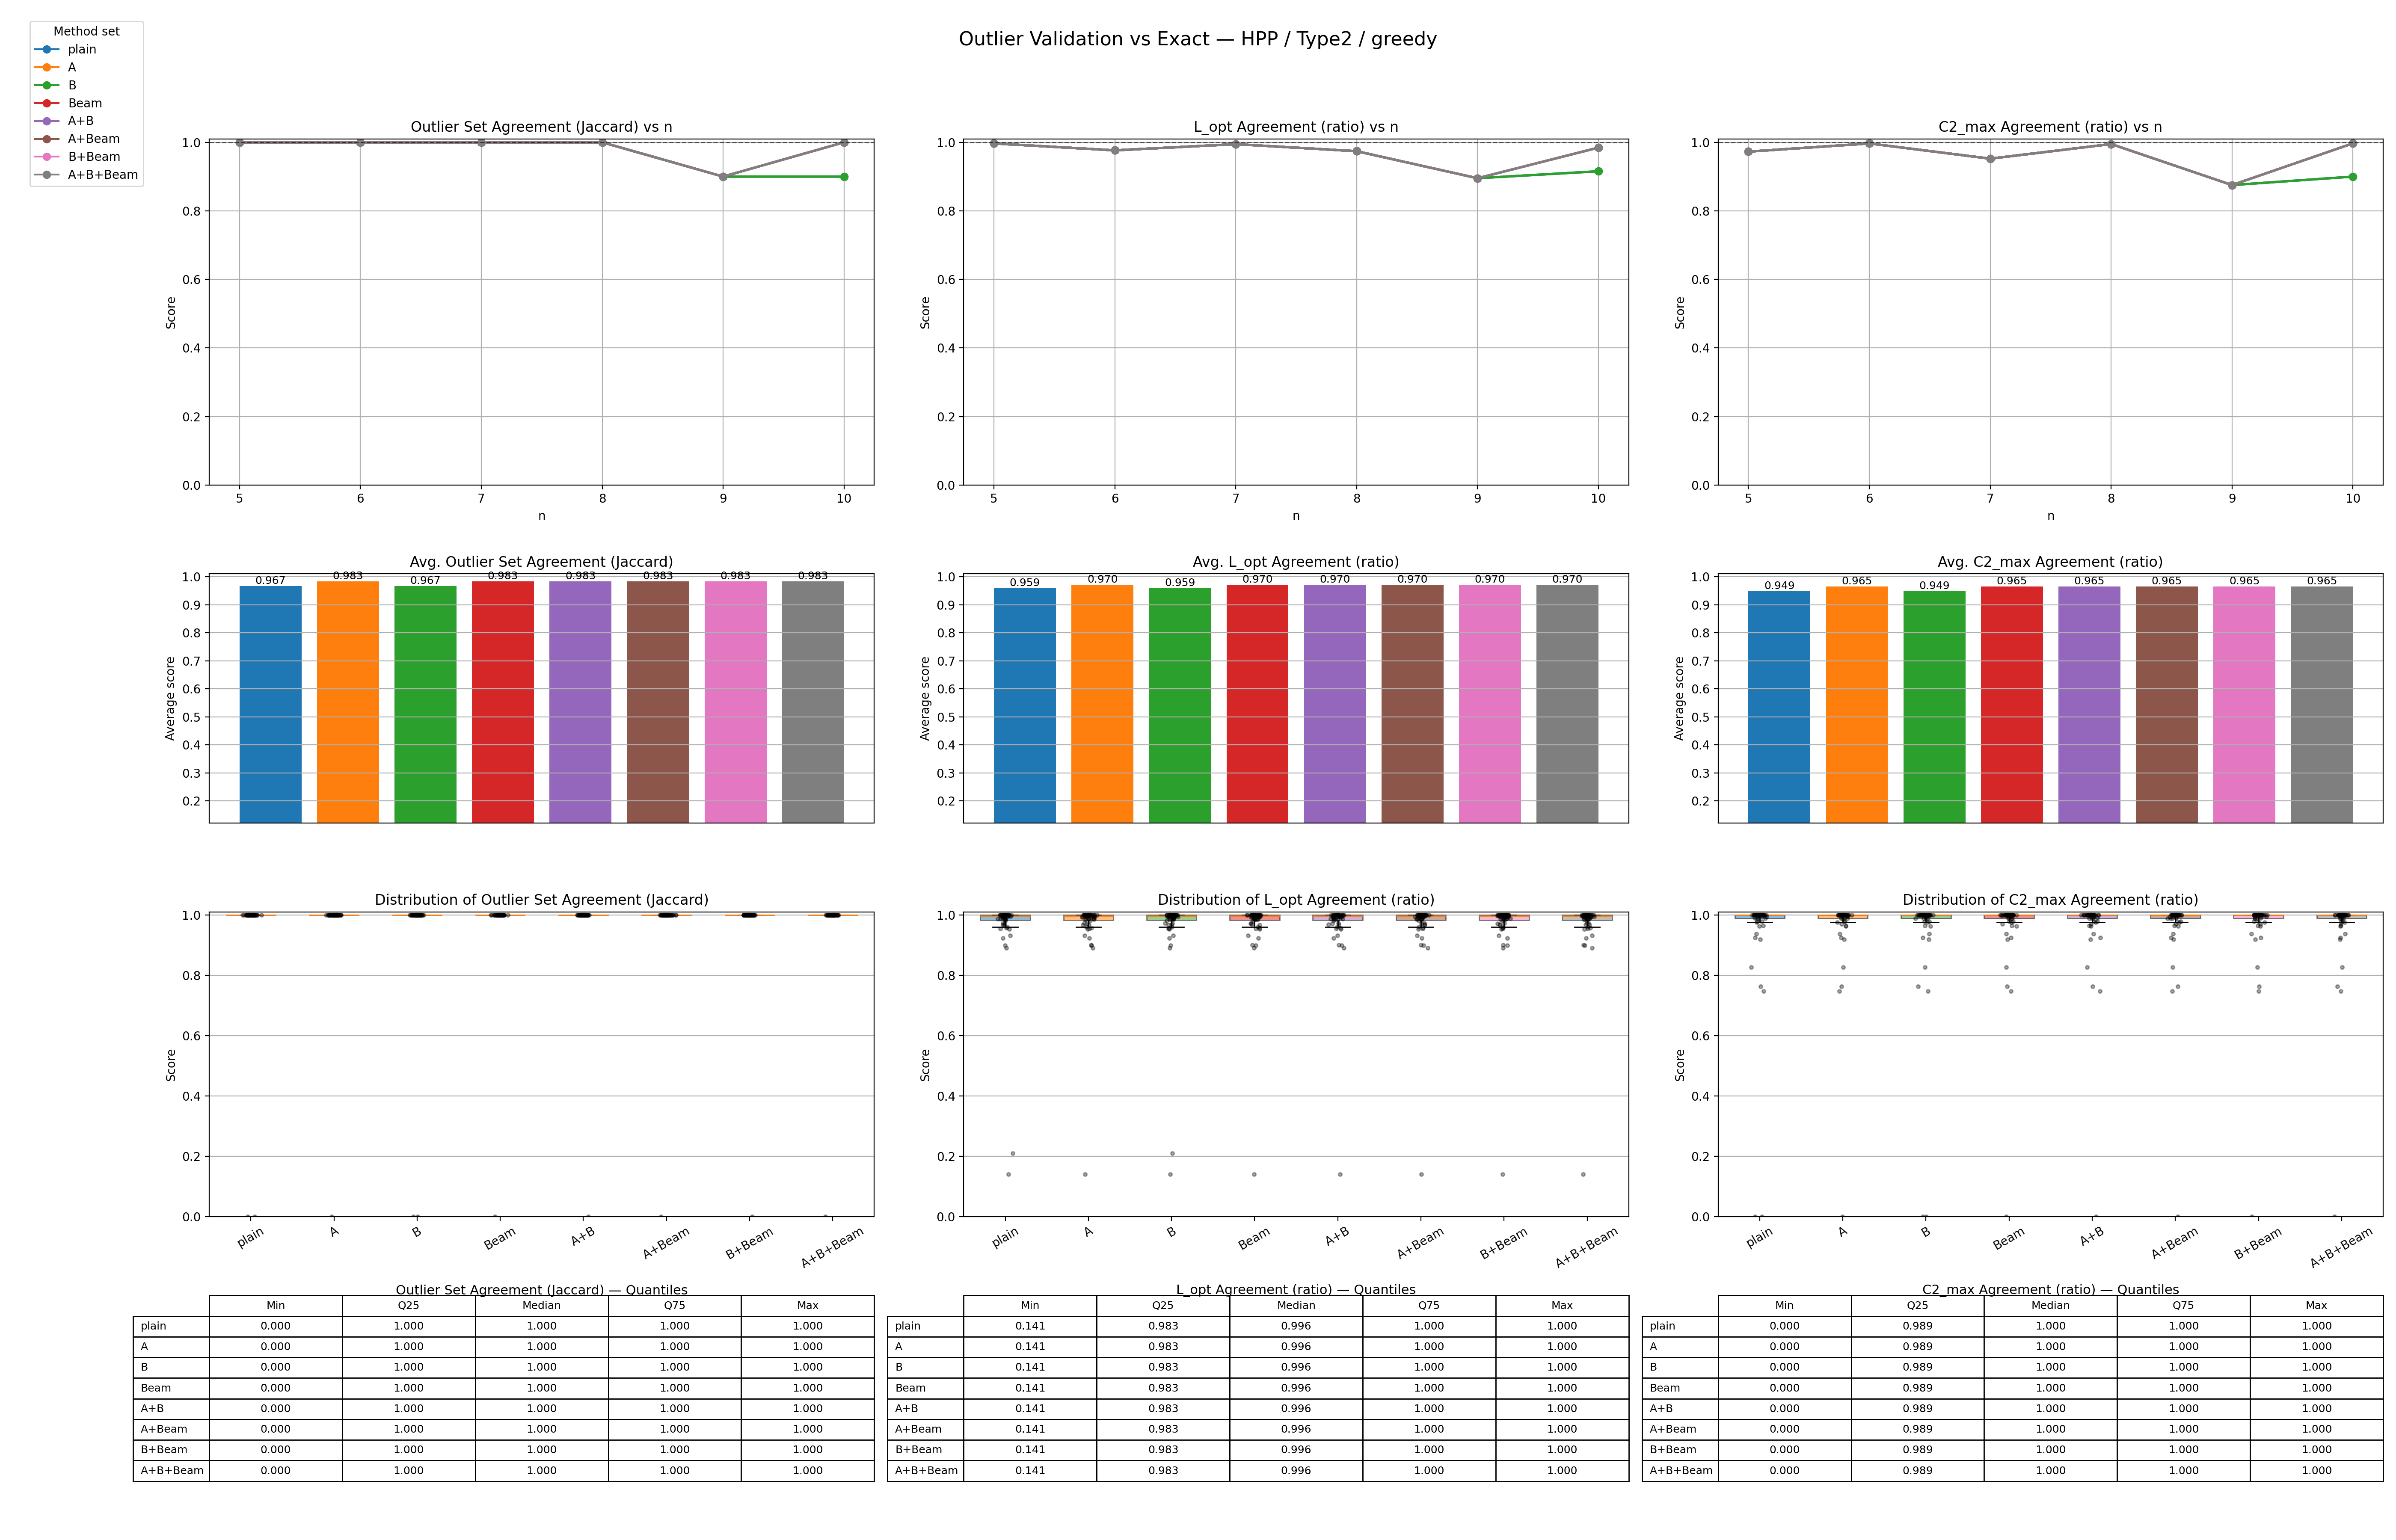
\includegraphics[width=\textwidth]{../../libraries/simulations/_img/validation/outliers/hpp/type2/greedy.png}
\caption{Detailed outlier-validation panel for HPP, Type~2, using \texttt{greedy}.}
\label{fig:appendix-hpp-type2-greedy-validation}
\end{figure}

\begin{figure}[p]
\centering
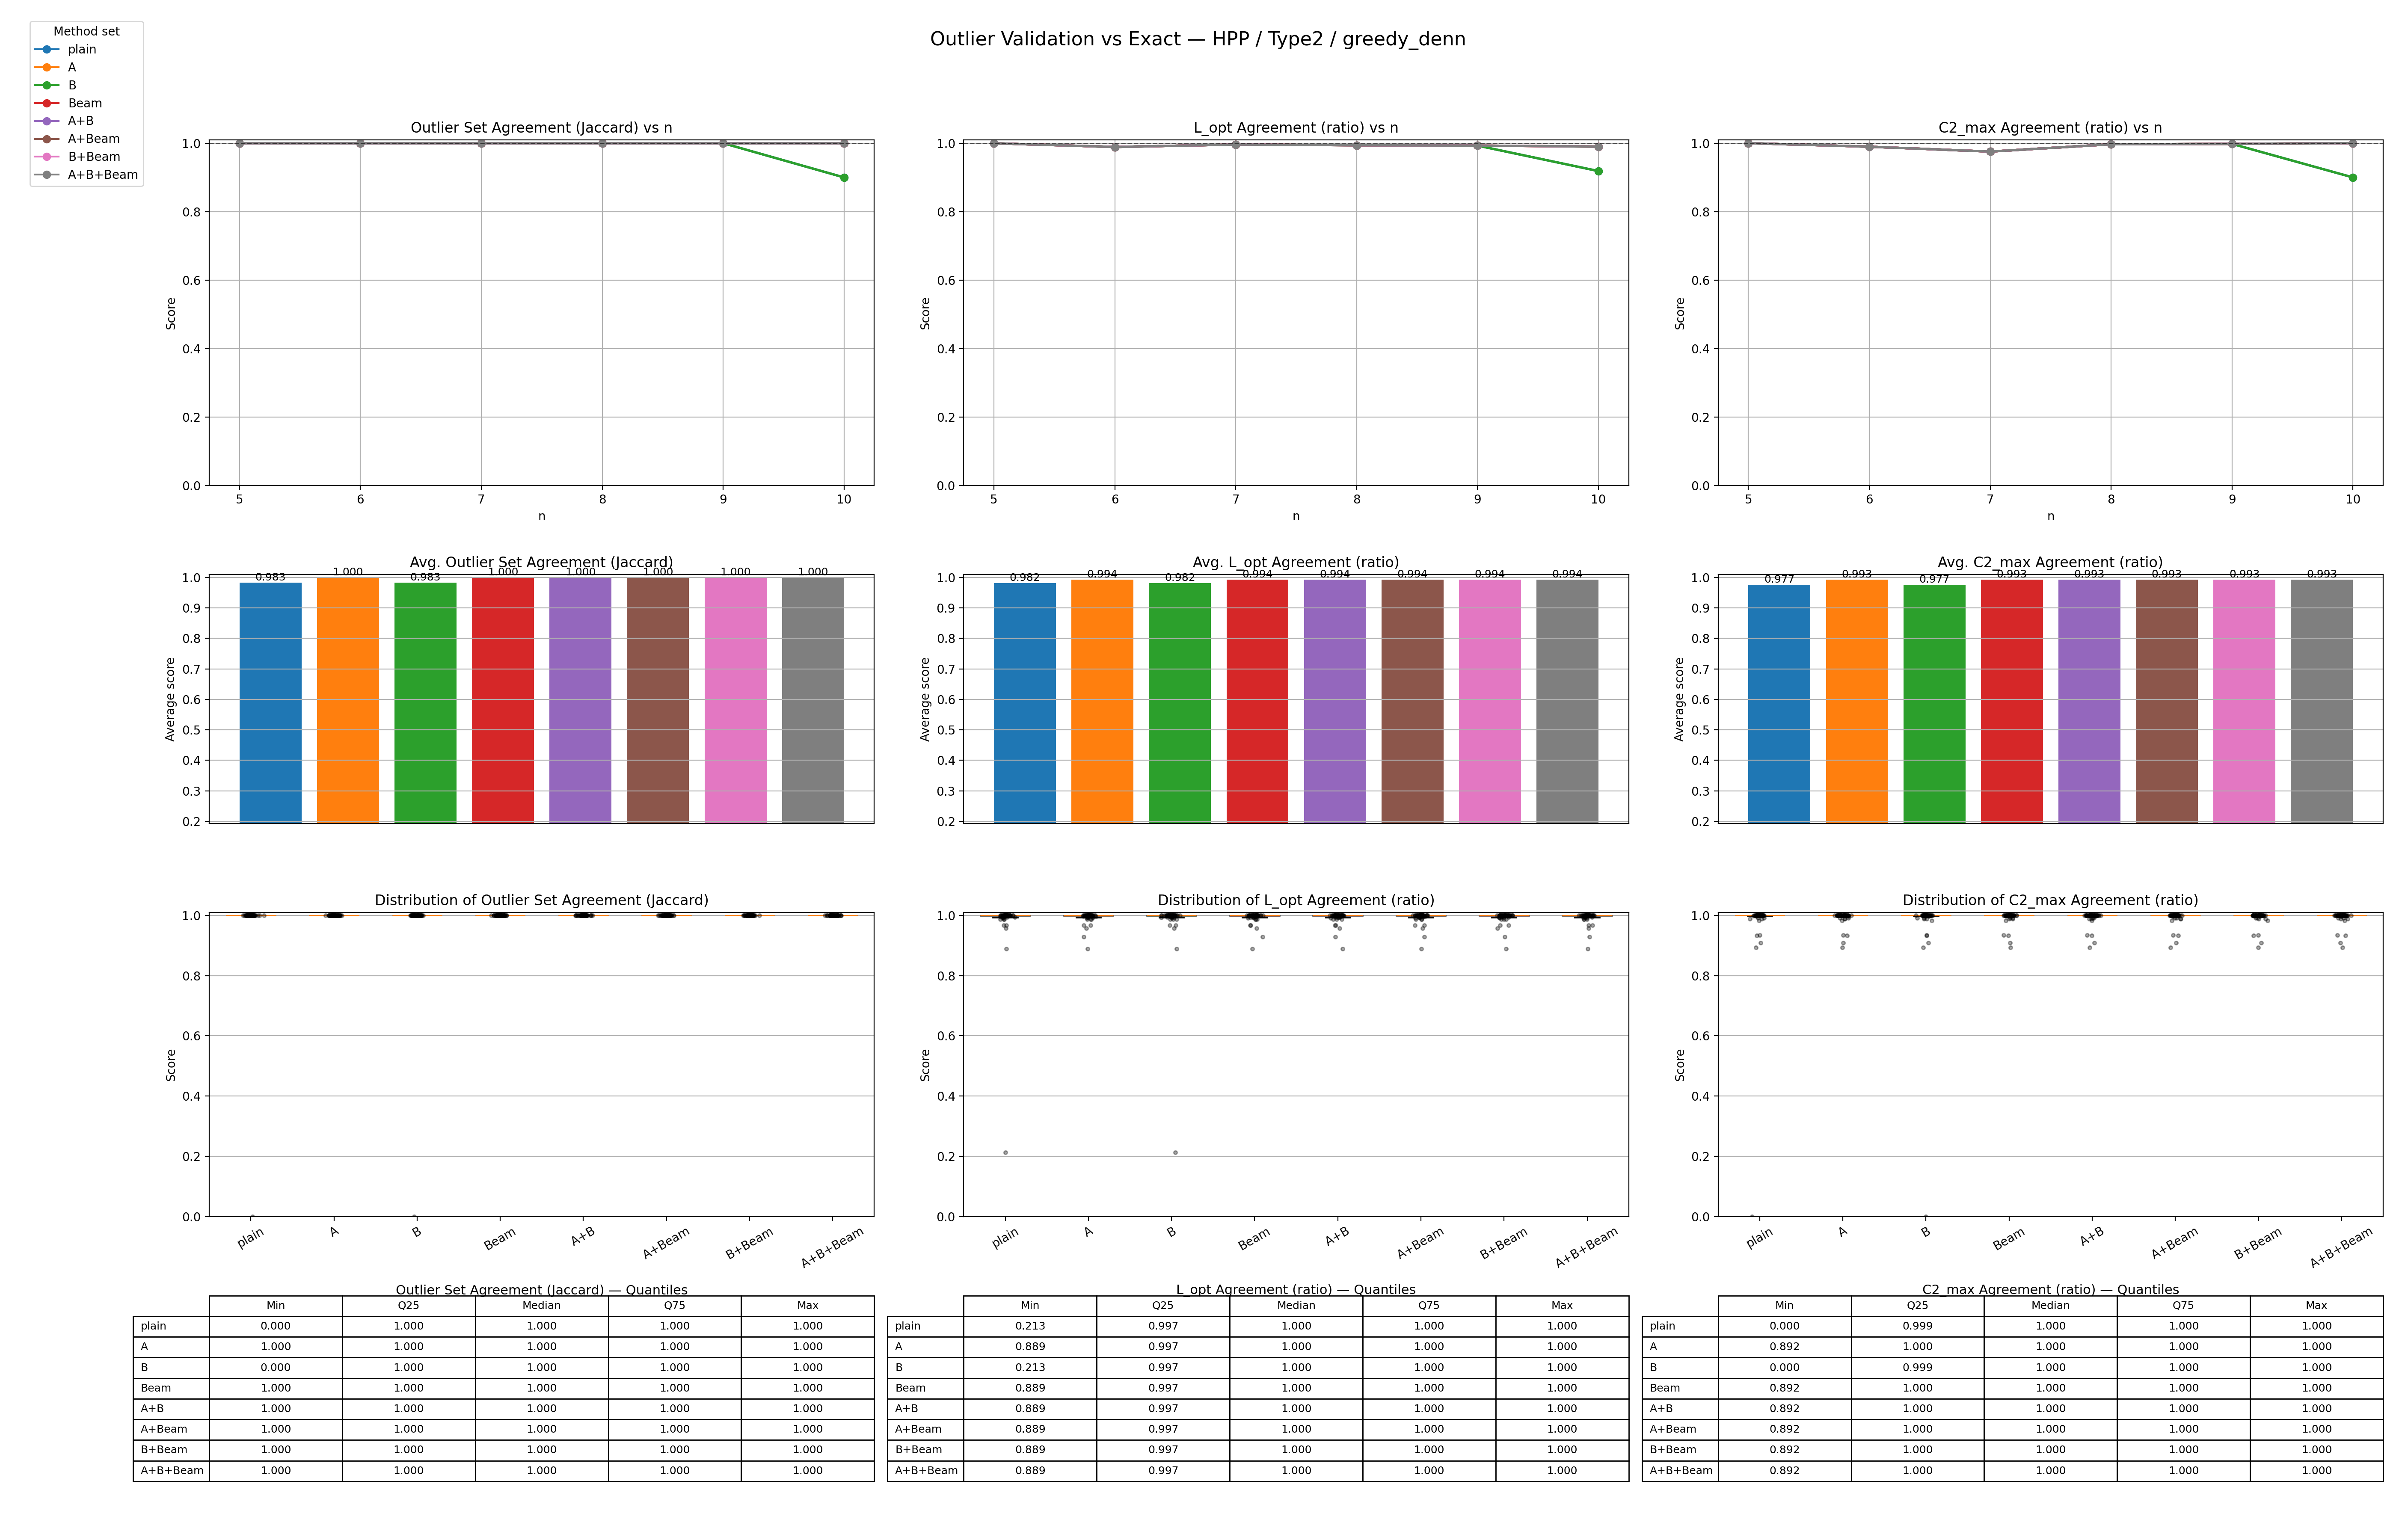
\includegraphics[width=\textwidth]{../../libraries/simulations/_img/validation/outliers/hpp/type2/greedy_denn.png}
\caption{Detailed outlier-validation panel for HPP, Type~2, using \texttt{greedy\_denn}.}
\label{fig:appendix-hpp-type2-greedy-denn-validation}
\end{figure}

\begin{figure}[p]
\centering
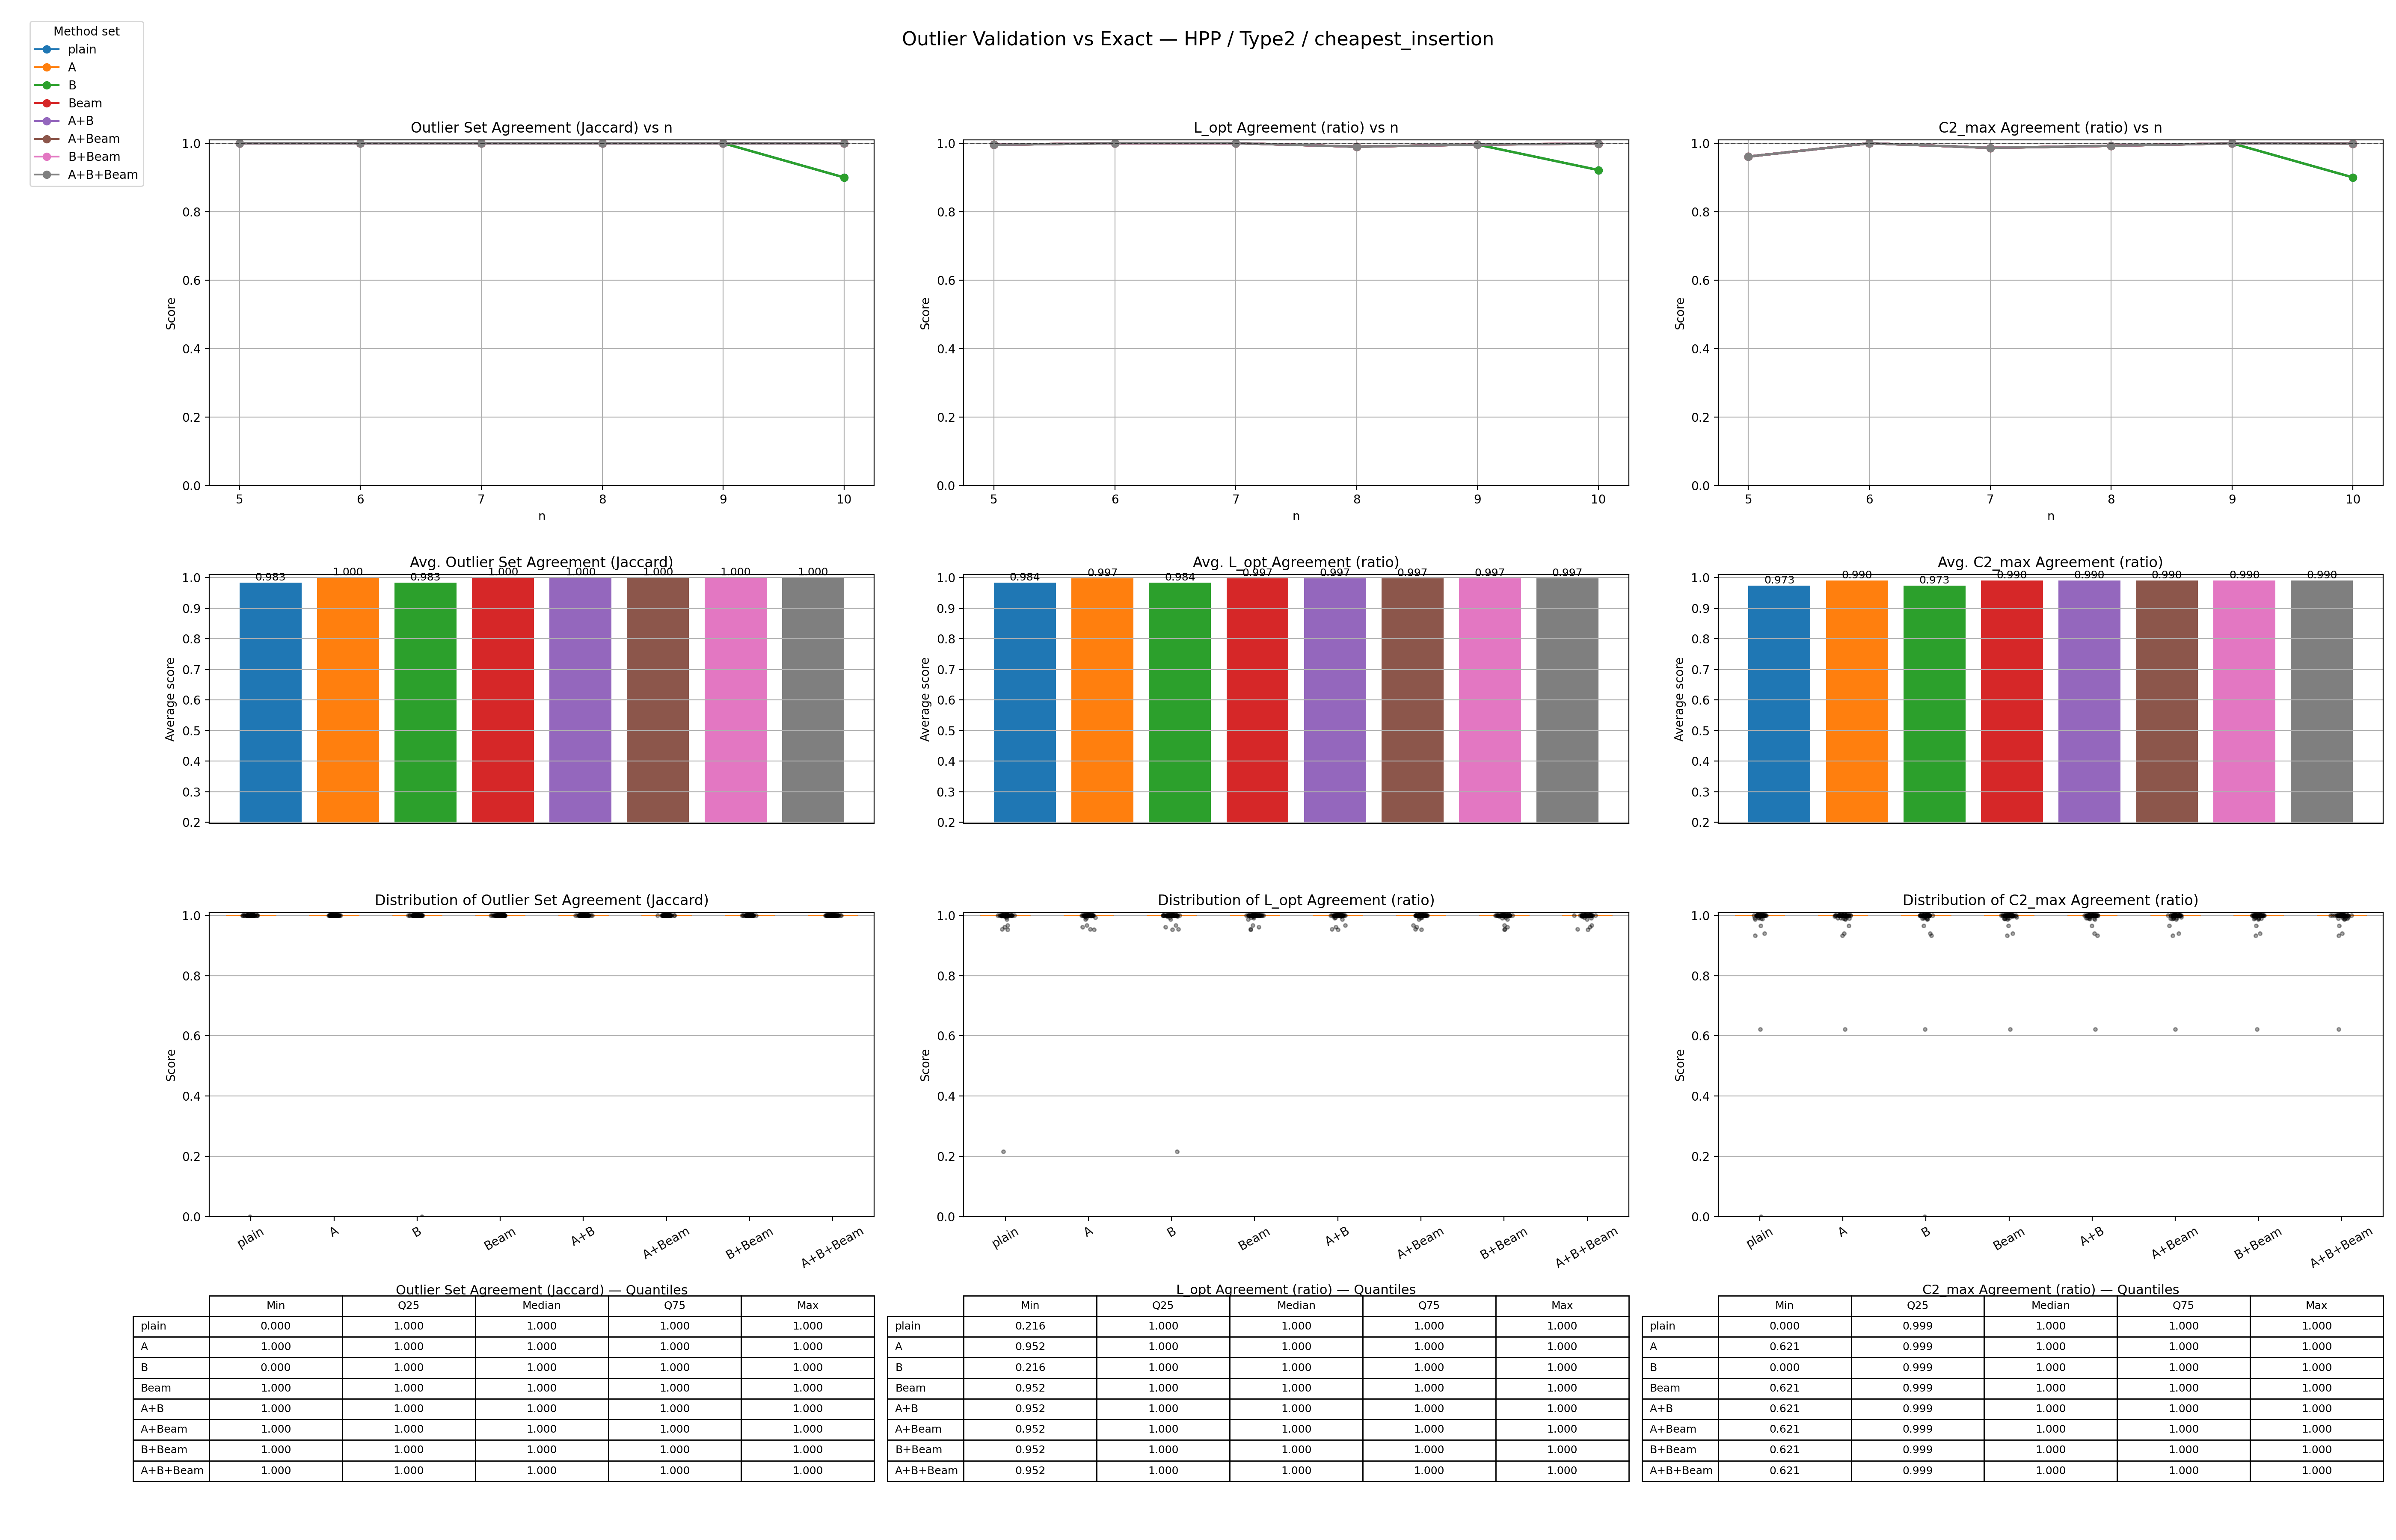
\includegraphics[width=\textwidth]{../../libraries/simulations/_img/validation/outliers/hpp/type2/cheapest_insertion.png}
\caption{Detailed outlier-validation panel for HPP, Type~2, using \texttt{cheapest\_insertion}.}
\label{fig:appendix-hpp-type2-cheapest-insertion-validation}
\end{figure}

\begin{figure}[p]
\centering
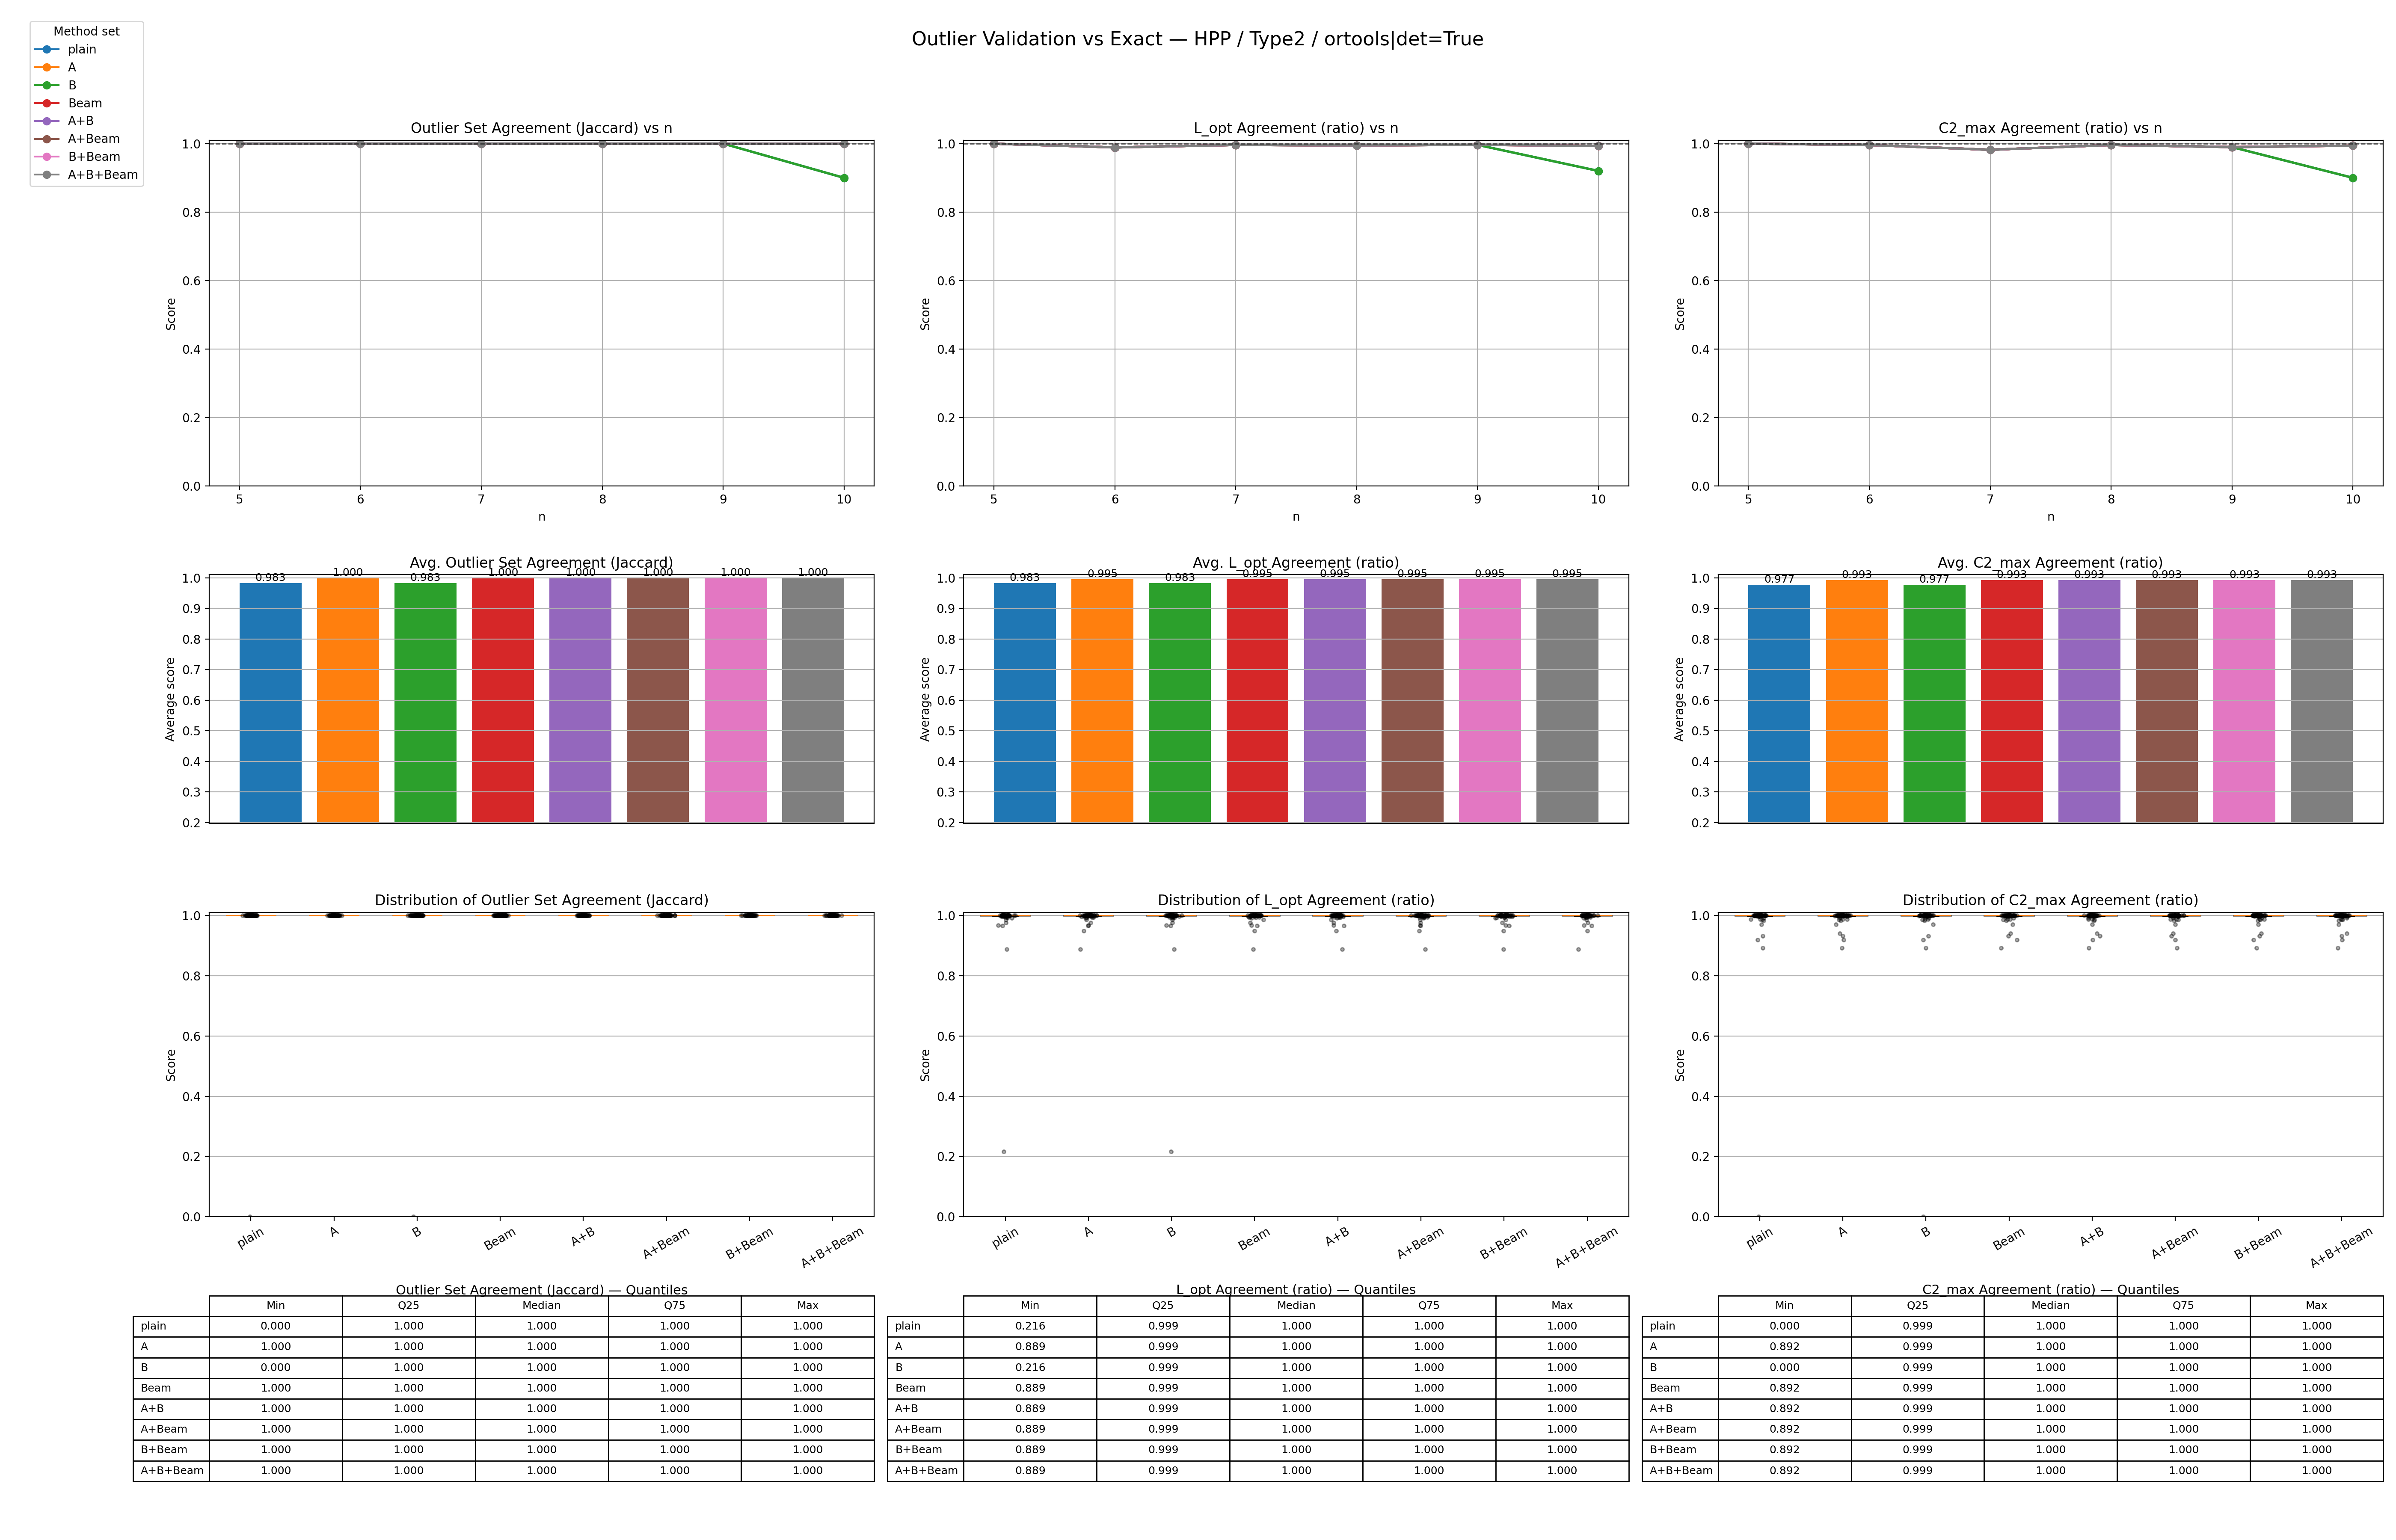
\includegraphics[width=\textwidth]{../../libraries/simulations/_img/validation/outliers/hpp/type2/ortools_detTrue.png}
\caption{Detailed outlier-validation panel for HPP, Type~2, using deterministic \texttt{ortools}.}
\label{fig:appendix-hpp-type2-validation}
\end{figure}

\begin{figure}[p]
\centering
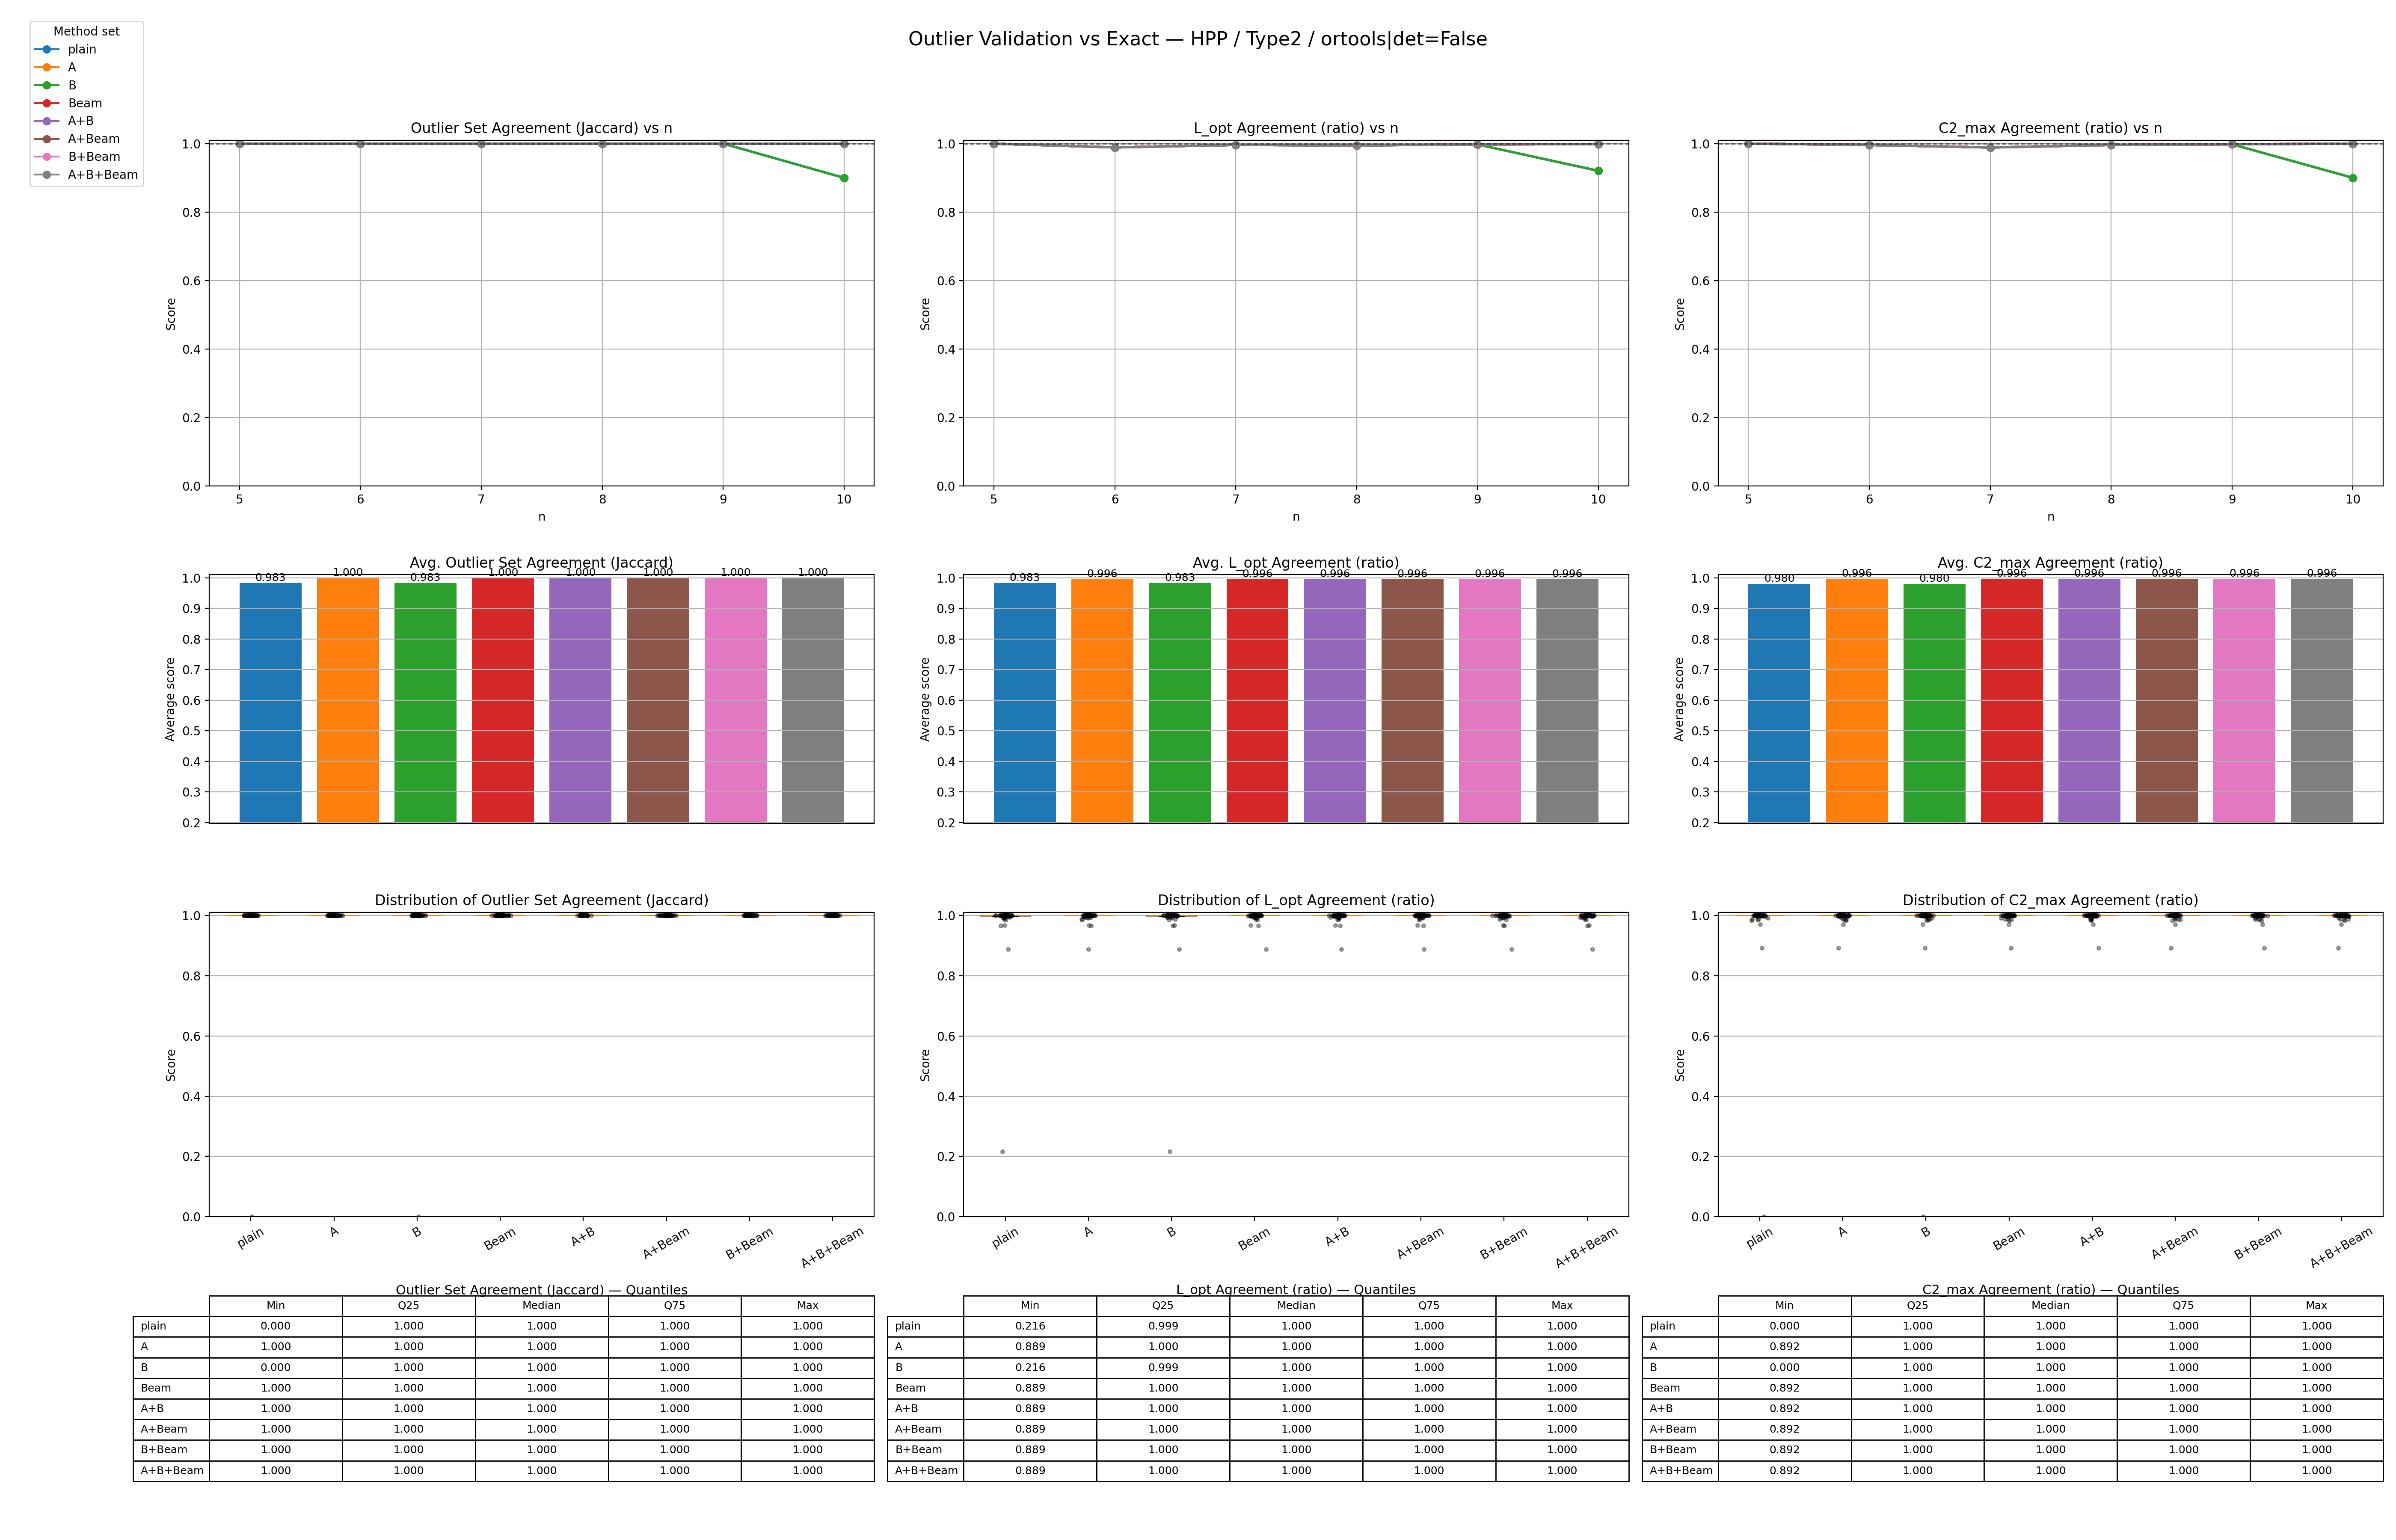
\includegraphics[width=\textwidth]{../../libraries/simulations/_img/validation/outliers/hpp/type2/ortools_detFalse.png}
\caption{Detailed outlier-validation panel for HPP, Type~2, using non-deterministic \texttt{ortools}.}
\label{fig:appendix-hpp-type2-ortools-det-false-validation}
\end{figure}

\end{document}
